%%%%%%%%%%%%%%%%%%%%%%%%%%%%%%%%%%%%%%%%%%%%%%%%%%%%%%%%%%%%%%%%%%%%%%%%%%%%%
%%%% Preamble
%%%%%%%%%%%%%%%%%%%%%%%%%%%%%%%%%%%%%%%%%%%%%%%%%%%%%%%%%%%%%%%%%%%%%%%%%%%%%

%%%% The uwthesis.sty file relies on the memoir class!
%%%% You should be using the memoir class anyway; it makes life easier:
%%%% http://www.ctan.org/tex-archive/macros/latex/contrib/memoir/


\documentclass[oneside, letterpaper, 12pt, oldfontcommands]{memoir}


\setsecnumdepth{subsubsection}

% Package imports and other setup
%!TEX root = ../nwoods_thesis.tex
% chktex-file 41

\usepackage{includes/uwthesis}
\usepackage{includes/ptdr-definitions}
\usepackage{graphicx}
\usepackage{amsfonts}
\usepackage{mathrsfs}
\usepackage{amsmath}
\usepackage{amssymb}
\usepackage{textcomp}
\usepackage{gensymb}
\usepackage{xspace}
\usepackage{booktabs}
\usepackage{caption}
\usepackage[utf8]{inputenc}

%%% Line numbering. Comment entire following block to remove
\usepackage{lineno}
% reset for each chapter
\usepackage{chngcntr}
\counterwithin*{linenumber}{chapter}
% silliness to make line numbers work before equations
\newcommand*\patchAmsMathEnvironmentForLineno[1]{%
  \expandafter\let\csname old#1\expandafter\endcsname\csname #1\endcsname
  \expandafter\let\csname oldend#1\expandafter\endcsname\csname end#1\endcsname
  \renewenvironment{#1}%
     {\linenomath\csname old#1\endcsname}%
     {\csname oldend#1\endcsname\endlinenomath}}%
\newcommand*\patchBothAmsMathEnvironmentsForLineno[1]{%
  \patchAmsMathEnvironmentForLineno{#1}%
  \patchAmsMathEnvironmentForLineno{#1*}}%
\AtBeginDocument{%
\patchBothAmsMathEnvironmentsForLineno{equation}%
\patchBothAmsMathEnvironmentsForLineno{align}%
\patchBothAmsMathEnvironmentsForLineno{flalign}%
\patchBothAmsMathEnvironmentsForLineno{alignat}%
\patchBothAmsMathEnvironmentsForLineno{gather}%
\patchBothAmsMathEnvironmentsForLineno{multline}%
}

\usepackage[hidelinks]{hyperref}
\usepackage[
  sorting=none,
  backend=biber,
  style=ieee,
  citestyle=numeric-comp
]{biblatex}

\usepackage{feynmp-auto}
\usepackage{breakurl}

\hypersetup{
  colorlinks,
  allcolors=black
}

\setsecnumdepth{subsubsection}
\maxtocdepth{subsubsection}

% Collaboration instead of author if present
\DeclareSourcemap{
  \maps[datatype=bibtex,overwrite=true]{
    \map{
      \step[fieldsource=collaboration,% fieldvalue={$1 Collaboration},
            final=true]
      \step[fieldset=usera, origfieldval, final=true]
    }
  }
}
\renewbibmacro*{author}{
  \iffieldundef{usera}{
    \printnames{author}
  }{
      \printfield{usera} Collaboration
  }
}

\DeclareFieldFormat{url}{\url{#1}}

\makeatletter
\DeclareFieldFormat{eprint:arxiv}{%
  arXiv\addcolon\space % chktex 1
  \ifhyperref % chktex 1
    {\href{http://arxiv.org/\abx@arxivpath/#1}{%
       \nolinkurl{#1}%
       \iffieldundef{eprintclass}
     {}
     {\addspace\mkbibbrackets{\thefield{eprintclass}}}}}
    {\nolinkurl{#1}
     \iffieldundef{eprintclass}
       {}
       {\addspace\mkbibbrackets{\thefield{eprintclass}}}}}
       \makeatletter
\renewcommand{\counterwithin}{\@ifstar{\@csinstar}{\@csin}}
\makeatother

% Symbols and a few functions
\newcommand{\lqcd}{\ensuremath{\Lambda_{\mathrm{QCD}}}}
\newcommand{\muF}{\ensuremath{\mu_{\mathrm{F}}}}
\newcommand{\muR}{\ensuremath{\mu_{\mathrm{R}}}}
\newcommand{\eee}{\ensuremath{\rm eee}}
\newcommand{\eem}{\ensuremath{{\rm ee}\mu}}
\newcommand{\mee}{\ensuremath{{\rm ee}\mu}}
\newcommand{\mme}{\ensuremath{\mu\mu {\rm e}}}
\newcommand{\emm}{\ensuremath{\mu\mu {\rm e}}}
\newcommand{\mmm}{\ensuremath{\mu\mu\mu}}
\newcommand{\VVV}{VVV}
\newcommand{\ETMISS}{\ptmiss}
\newcommand{\W}{\PW\xspace}
\newcommand{\ZZ}{\cPZ\cPZ\xspace}
\newcommand{\WW}{\PWp\PWm\xspace}
\newcommand{\WZ}{\cPW\cPZ\xspace}
\newcommand{\WWZZ}{\cPW\cPW\cPZ\cPZ\xspace}
\newcommand{\tZq}{{\cPqt}Zq\xspace}
\newcommand{\jet}{\ensuremath{\mathrm{j}}\xspace}
\newcommand{\zepl}{\ensuremath{\eta^{3\ell} - \frac{1}{2}(\eta^{j_{1}} + \eta^{j_{2}})}}
\newcommand{\etas}{\ensuremath{\eta^{*}_{3\ell}}}
\newcommand{\mjj}{\ensuremath{m_{\mathrm{jj}}}}
\newcommand{\EWWZ}{EW WZ\xspace}
\newcommand{\WZjj}{\ensuremath{\rm {WZjj}}\xspace}
\newcommand{\QCDWZ}{QCD WZ\xspace}
\newcommand{\etajj}{\ensuremath{\Delta\eta_{\mathrm{jj}}}}
\newcommand{\detajj}{\ensuremath{\Delta\eta(\mathrm{j}_{1}, \mathrm{j}_{2})}}
\newcommand{\MG} {\textsc{MadGraph5\_aMC@NLO}\xspace}
\newcommand{\VBFNLO}{{\sc Vbfnlo}\xspace}
\newcommand{\MoCaNLO}{M\protect\scalebox{0.8}{oCaNLO}\xspace}
\newcommand{\Recola}{R\protect\scalebox{0.8}{ecola}\xspace}
\newcommand{\Moca}{\textsc{\protect{{M\protect\scalebox{0.8}{oCaNLO}\xspace}+{R\protect\scalebox{0.8}{ecola}\xspace}}}}
\newcommand{\Sherpa}{\textsc{S\protect\scalebox{0.8}{HERPA}\xspace}}
\newcommand{\Rivet}{R\protect\scalebox{0.8}{IVET}\xspace}
\newcommand{\Herwig}{\HERWIG}
\newcommand{\Pythia}{\PYTHIA}
\newcommand{\FxFx}{{\sc FxFx}\xspace}
\newcommand{\Zpj}{\ensuremath{{\cPZ}\mathrm{+jet}}\xspace}
\newcommand{\lcand}{\ensuremath{\ell_{\rm candidate}}}
\newcommand{\mt}{\ensuremath{m_{\mathrm{T}}(\PW\cPZ)}}
\newcommand{\PHpm}{\ensuremath{\PH^{\pm}}}
\newcommand{\Uone}{U(1)}
\newcommand{\SUtwo}{SU(2)}
\newcommand{\PbT}{PbWO$_4$}
\newcommand{\pp}{\Pp\Pp\xspace}

% add the biblography we'll use
\addbibresource{bibliography.bib}

% Define what goes on the title page and in the abstract (but don't actually create them yet)
\settitle{Measurement of electroweak $\PW\PZ$ boson production and search for new physics in proton-proton collisions at $\sqrt{s} = 13\TeV$ with the CMS detector at the CERN LHC}
\setauthor{Kenneth Long}
\setdepartment{Physics}
\doctors % or \masters
\setgraddate{2019}
\setdefensedate{20 April 2019} 

%%%% Members of the Final Oral Committee (FOC)
%%%% Give name, rank, and department
%%%% 
\setfoca{Matthew Herndon}{Professor}{Physics} % <- Your advisor
\setfocd{Tulika Bose}{Professor}{Physics}
\setfocc{Sridhara Dasu}{Professor}{Physics}
\setfocb{Lisa Everett}{Professor}{Physics}
\setfoce{Ellen Zweibel}{W. L. Kraushaar Professor}{Physics and Astronomy}


\setabstract{
A measurement of electroweak (EW) 
$\WZ$ boson production via vector boson scattering is presented.
The measurement is performed in the leptonic decay modes $\WZ \to \ell\nu\ell'\ell'$,
where $\ell, \ell'$ indicate and electron or muon.
The analysis is based on a data sample of proton-proton
collisions at $\sqrt{s} = 13\TeV$ at the 
CERN Large Hadron Collider collected with the 
Compact Muon Solenoid detector and corresponding to an integrated luminosity of $35.9\fbinv$.
The \WZ plus two jet production cross section
is measured in fiducial regions with enhanced contributions from
\EW production and found to be consistent with standard model predictions.
The \EWWZ production in association with two jets is measured with an observed (expected) significance of 2.2 (2.5) standard deviations.
Results are also interpreted in terms of physics beyond the standard model modifying the 
interactions of the $\PW$ and $\PZ$ bosons.
Constrains on charged Higgs boson production and on anomalous quartic gauge couplings in terms of
dimension-eight effective field theory operators are presented.
}



%%%%%%%%%%%%%%%%%%%%%%%%%%%%%%%%%%%%%%%%%%%%%%%%%%%%%%%%%%%%%%%%%%%%%%%%%%%%%
%%%% Document
%%%%%%%%%%%%%%%%%%%%%%%%%%%%%%%%%%%%%%%%%%%%%%%%%%%%%%%%%%%%%%%%%%%%%%%%%%%%%

\begin{document}

%% Tell the memoir class to set up lowercase roman for pagination, etc.
\frontmatter


% The title page
\thetitlepage{}
\clearpage

% The copyright page, if you want to pay the fee and register copyright.
% \thecopyrightpage
\cleardoublepage{}

% These above pages should not be counted, so we reset the counter to 1.
\setcounter{page}{1}

% An abstract may be required by your department.
\section{Abstract}
\uwabstract{}
\cleardoublepage{}

% Acknowledgements go here if you want to include them.
\section{Acknowledgements}
%\section{Acknowledgements}

I would like to sincerely thank my thesis advisor, Matthew Herndon.
I am grateful for your guidance, 
You directed me to projects 
gave me freedom to explore 
I must also thank Wesley Smith and Sridhara Dasu.
You who held me to the same high standards you expect of your own 
students---I won't say I always enjoyed this, but I am very grateful for it.


\clearpage

% Table of contents
\tableofcontents*
% \clearpage

\makeatletter
     \renewcommand*\l@figure{\@dottedtocline{1}{1em}{3.2em}}
\makeatother

 \clearpage
 \listoffigures  % if you have any figures
 \listoftables   % if you have any tables

% Tell the memoir class to set up normal pagination, etc. for the main doc
\mainmatter{}


%%%%%%SETLINE NUMBERS
\setpagewiselinenumbers
 \modulolinenumbers[1]
 \linenumbers % chktex 1
%%%%%%%END SETLINE NUMBERS

% Chapters

\chapter{Introduction}
\label{ch:introduction}

This thesis presents measurements of the production of events with
three leptons, two forward ``jets'' of clustered hadronic particles,
with an imbalance of transverse momentum. 
Events are selected to isolate contributions involving the simultaneous
production of a $\PW^{+}$ or $\PW^{-}$ and $\PZ$ boson, the heavy particles
that communicate the weak force.
Selected events are used
to measure the rate of production of processes predicted by the standard
model (SM) of particle physics, the most complete theoretical expression
of the known particles and forces of the universe, and to search for hypothetical extension
of the SM. 

A dedicated search
for a rare, previously unobserved, SM process, referred to as electroweak
WZ (\EWWZ) production, is presented. 
The presence and production rate of the \EWWZ process is intimately connected to the 
phenomenon of EW symmetry breaking (EWSB) \cite{Quigg:2009vq}, which leads to 
the W and Z bosons acquiring masses
and self-interactions. A fundamental prediction
of EWSB, fulfilled in the standard model (SM) by the Brout-Englert-Higgs (BEH) mechanism,
is the emergence of a scalar particle, known 
to as the Higgs boson. 
This particle was first observed by the 
ATLAS~\cite{Aad:2012tfa} and CMS~\cite{Chatrchyan:2012xdj,Chatrchyan:2013lba} Collaborations
at CERN in 2012, providing compelling evidence for the BEH mechanism as
a component of the SM theory.

In addition, constraints on physics beyond the SM (BSM) are placed on in terms
of explicit models predicting charged Higgs bosons decaying to a $\Wpm$ and a $\PZ$
boson, and on

\section{The universe of particles}

The idea of understanding the physical world by identifying its
fundamental constituents is a very old one. Ancient eastern and
western philosophers independently attempted the feat, concluding
that the world could be reduced 
to ``elements'' such as water, earth, and fire.
As observational science became a more prominent component of modern thought, 
evidence mounted that these elements themselves were 
not indivisible. Perhaps the Greeks had not identified
the correct fundamental elements, but the belief that this endeavor could
be accomplished lived on.

A major attraction of identifying the fundamental building blocks of the universe
is the implication for constructing a macroscopic description from these
pieces. This process of understanding a complex system 
by reducing it to its essential components
termed ``reductionism'' by philosophers, 
has formed the backbone of scientific endeavor for much of history.
In practice, the step from the fundamental to the macroscopic 
is far from trivial. Despite a well-established
understanding of the proton constituents and their interactions,
predicting the proton mass from first principles has only recently 
been achieved~\cite{Durr:2008zz}, and larger systems remain well
out of reach.
In addition to the challenges of calculability, additional structures
may arise from the nature of large systems, such as ferromagnetism or 
superconductivity.
This long-accepted path to a complete description of the physical world
has thus been called into question, and it may never be feasible
to achieve a theory of biology built from the findings of particle 
physics~\cite{Anderson393}.
Yet there is an undeniable elegance in achieving a concise description
of the fundamental elements of the natural world and their interactions,
and this remains the target of the field of particle physics today. 

The modern genesis of the field can perhaps be credited to 
the discovery of the electron in 1897 by J. J. Thomson, a particle still
believed to be elementary today.
Further experiments showed that the electron carries the smallest quantity of electric charge found
freely in nature, and we now know that many macroscopic electrical phenomena
arise from the motion of electrons in atoms.
A mathematical understanding of these electromagnetic interactions had 
already been established by James Clerk Maxwell decades before Thompson's work
The idea of a particle of light is therefore seemingly at odds with Maxwell's theory,
which described light as a oscillations of electromagnetic fields,
but a quanta of light was central to the explanation of black-body radiation provided by Max Planck 
and for the theoretical explanation of the photoelectric effect developed by Albert Einstein.
The theory of fields and particle-like characteristics of electromagnetic
interactions were reconciled shortly after these proposals by the 
rapidly-developing quantum theory.
The quanta of light, the photon, is now understood to communicate the electromagnetic force.
By the early 1940s, these pieces had evolved into the theory of quantum 
electrodynamics, the first
quantized theory of particles and their interactions in the language 
of quantum field theory. 

Simultaneous to the efforts to develop a mathematical language to describe 
the fundamental particles and their interactions was an experimental effort 
to find and categorize them. New equipment for detecting these particles,
such as the cloud chamber developed by Charles Wilson, 
gave a perspective on the spontaneous 
decay of atoms and opened our eyes to the radiation bombarding the earth from
outside the atmosphere. By the 1950s, particle physicists were faced with a ``particle zoo''
of seemingly fundamental objects spanning a huge range of masses. 
An underlying structure of the properties of many of these particles, 
now known as hadrons, was described by Murray Gell-Man and George Zweig in 1964.
They realized the properties of the many observed hadrons could be 
attributed to combinations of different elementary particles,
which Gell-Man termed quarks.
Whether these particles were physical entities or abstractions was 
not immediately evident, but experiments at the Stanford Linear Accelerator
at the end of the 1960s showed the proton to have point-like constituents
with the properties Gell-Man and Zweig predicted.

Despite the progress in explaining the structure of hadronic matter,
it remained unclear that the language of a quantum gauge theory, 
so successful in the formulation of the electromagnetic interaction, could 
also describe the strong nuclear force responsible for the formation
of these composite particles, and the weak nuclear force responsible for
a subset of their decays. Both exhibited striking differences with
respect to the electromagnetic interaction:
the weak nuclear force acts over a much smaller distance, while
the strong nuclear 
force has an inverted scaling with distance, increasing at higher separation
of the interacting objects while decreasing at very short ranges. 

A unification of the electromagnetic and weak nuclear force was achieved
by Sheldon Glashow, Abdus Salam, and Steven Weinberg in the early 1970s.
A crucial component of their theory is the presence of a scalar field, 
which gives mass to the W and Z bosons through EWSB, leading to the 
short range of the weak force.
A description of the strong nuclear force as a quantum 
gauge theory followed,
with the inverse distance scaling properties of the theory,
termed quantum chromodynamics (QCD), demonstrated by
David Gross, David Politzer and Frank Wilczek.
The discovery of the gluon, the so-called gauge boson of the theory,
in 1979 at the Deutsches Elektronen-Synchrotron (DESY) in Hamburg, Germany
provided definitive confirmation
of gauge theory as the theoretical foundation of the particle physics.
The outstanding prediction of the 
electroweak theory, that the W and Z bosons which communicate the weak 
interaction acquire mass through the presence of scalar field, required
longer for experimental confirmation. This confirmation arrived a half-century
later, with the observation of the Higgs boson at CERN in 2012.
Together, the description of these interactions and the particle content
and these interactions described by the EW and QCD theories are known
as the standard model of particle physics.

\begin{figure}[htbp]
  \centering
   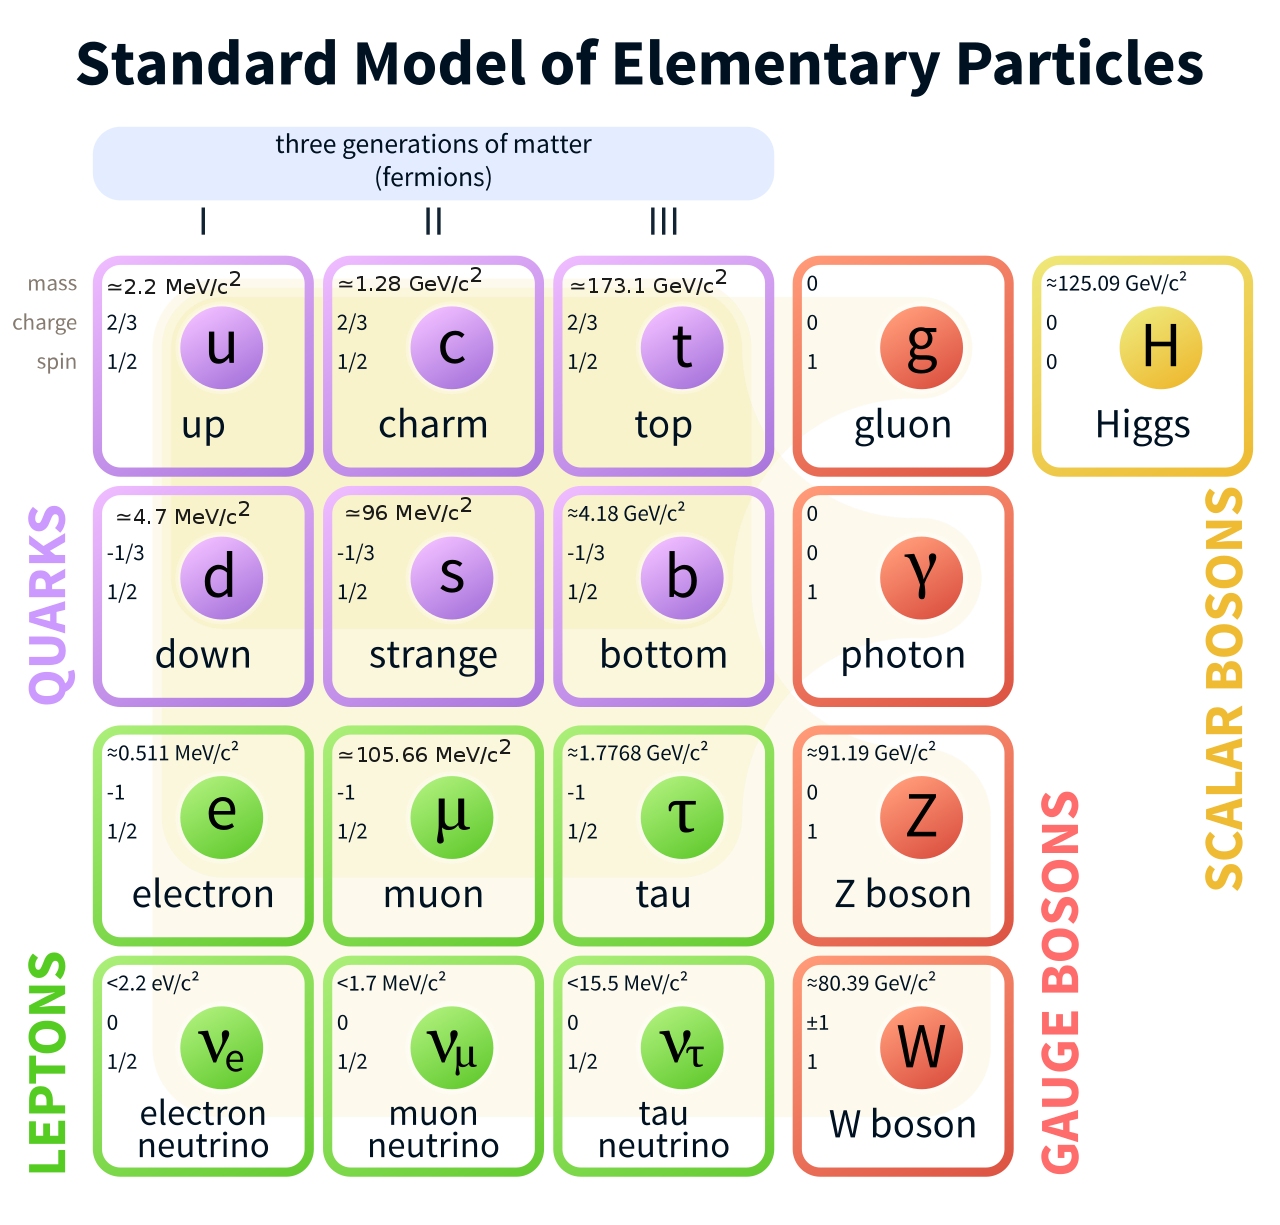
\includegraphics[width=0.9\textwidth]{figures/Chapter1/ChartOfParticles.png}
  \caption{
    The experimentally established particle content of the universe.
  }
 \label{fig:theparticles}
\end{figure}

The currently known particle content of the universe is depicted in Fig.~\ref{fig:theparticles}.
The quarks, highlighted in green, and leptons, highlighted in purple,
form matter, while the vector bosons, highlighted in red, mediate the 
interactions of this matter. The Higgs particle, shown in yellow,
has a unique role in the SM. It arises from the Higgs field, which
leads to masses for the W and Z bosons as well as the quarks and leptons.
The underlying mathematical framework used to understand the quantum 
properties of these particles and their interactions will be further discussed
in Chapter~2. 

\textbf{Go ahead and expand the description of what the particles are in this section}.

\section{Particle collider experiments}
\textbf{Introduce idea of scattering experiment}
\textbf{Introduce idea of cross section}

To observe the smallest pieces of matter, one must break matter into pieces.
The discovery of radioactivity in the late 1800s by Henri Becquerel had
profound implications for this idea, as it represented the spontaneous
disintegration of atoms. 
In addition to studying the products of these decays themselves, 
Earnest Rutherford realized the energetic decay products could be used
to perform the first particle scattering experiments. By directing the 
helium nuclei emitted from radioactive radium decay towards gold foil
and measuring the deflection
angles, he and his collaborators established the existence of the atomic nuclei.
Inferring information about the properties and interactions of particles based on their
behaviour when scattered is still central to particle physics experiment today.

Rutherford continued to use the radioactive decays of elements as a means
for particle acceleration in the early 1900s. Yet it was clear that
a means of accelerating collisions to higher energies would be needed
to continue to probe the structure of the nucleus.
These efforst lead to the invention of the 
the first particle accelerators, which have come to define the field ever since.
An electrostatic accelerator was developed at the Cavendish Laboratory
in Cambridge, England by John Crockhoff and Ernest Walton and
was used to split Lithium into Helium atoms in 1932.
Concurrently, Ernest Lawrence developed the cyclotron in California,
which became a model for many future accelerator facilities.

These inventions triggered an explosion in the field, marked by a continual 
effort to collide particles at higher and higher energies. Many major discoveries
are closely linked with technological advancements or collaborative
efforts leading to more powerful accelerators.
The facilities at the European Center for Nuclear
Research (CERN), DESY, and at the 
Fermi National Accelerator Laboratory (Fermilab) in Illinois
are strongly associated with the 
discoveries they enabled, including evidence for the force carries
of the EW and QCD interactions, the W and Z bosons and the gluon.

The most powerful collider ever built, the LHC at CERN,
now allows the study of the most energetic particle collisions ever
recorded in the laboratory, reaching concentrated energies only replicated
in the most cataclysmic events in the universe. The LHC
was planned, developed, and built over the course of decades, with
personnel and funding from countries throughout the world.
This work is based on studies of pp collisions delivered by the LHC 
and collected by the Compact Muon Solenoid detector in 2016.

\textbf{Maybe explain a bit more what a scattering experiment is here}

The LHC and Compact Muon Solenoid detector are discussed in detail 
in Chapter~3 of this thesis.

\section{Motivation and context of this result}
The work presented in this thesis
has two related motivations: performing a measurement of a rare
process predicted by the SM, and searching for signs of 
BSM physics in a channel and topology sensitive to modifications of
the EW sector of the SM.
Characterizing the self-interactions of the vector bosons is an important
step to understanding the self-consistency of the SM, and a useful probe
of possible deviations from its predictions. Because the production of events
with multiple vector bosons in the final state
requires collisions with a high center of mass energy, the LHC has
the potential to explore these states in more depth 
than previously achieved.

Measurements of WW and WW$\gamma$ production in electron--positron collisions
were first made at the LEP
Collider at CERN by the ALEPH, DELPHI, L3, and OPAL Collaborations~\cite{LEP-2}.
These processes are sensitive to the triple vector boson couplings
WWZ and WW$\gamma$, and the quartic couplings WW$\gamma\gamma$
and WWZ$\gamma$. The production rate and angular distributions of the decay
products of the vector bosons in these states were used to derive values 
of the triple and quartic couplings. No deviations were observed from the 
predictions of the SM with a light Higgs boson.

Production of charged vector boson pairs was also studied in proton--antiproton
collisions at the Tevatron Collider at the Fermilab. 
The measurement of WZ production, inclusive in the
number of clustered hadronic particles -- referred to as jets (j), was
first performed by the CDF~\cite{Aaltonen:2012vu,Abulencia:2007tu} 
and D0~\cite{Abazov:2012cj} Collaborations at the Tevatron in 2006. 
Measurements of the WWZ coupling were found to be consistent with the results
from the LEP experiments and with the SM.

Experimental sensitivity to quartic couplings of the massive vector boson 
was first achieved at the LHC.
In pp collisions, quartic WZ interactions are accessible through triple 
vector boson production or through vector boson scattering (VBS), 
in which vector bosons are radiated from the quarks in the colliding protons 
before interacting.
These interactions include WZ quartic couplings, as shown in Fig.~\ref{fig:feynmanDiagrams}~(a). 
Constraints on the deviations of quartic couplings from the SM prediction, 
referred to as anomalous quartic gauge couplings (aQGC), in 
WZ events with at least two jets (\WZjj) were first
presented by the ATLAS collaboration at 8 TeV~\cite{Aad:2016ett}. This result
is the first study of WZ vector boson scattering at CMS. 

\begin{figure}[htbp]
  \centering
   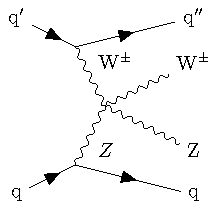
\includegraphics[page=1,width=0.25\textwidth]{figures/FeynmanDiagrams/feynmanVBS.pdf}
   \includegraphics[page=2,width=0.25\textwidth]{figures/FeynmanDiagrams/feynmanVBS.pdf}
   \includegraphics[page=3,width=0.25\textwidth]{figures/FeynmanDiagrams/feynmanVBS.pdf}
  \caption{Representative Feynman diagrams for \WZjj production in the SM and BSM. 
  EW-induced WZ production includes quartic interactions (a) of the vector bosons.
  New physics in the EW sector modifying the quartic coupling 
  can be parameterized in terms of dimension-eight effective field theory operators (b).
  Specific models modifying this interaction include those predicting charged Higgs bosons (c).
  }
 \label{fig:feynmanDiagrams}
\end{figure}

A well-motivated modification of the WWZZ quartic coupling would arise from
the presence of charged Higgs bosons.
In the SM, EWSB is fulfilled by a single Higgs field, which transforms as an SU(2) doublet.
Extending the Higgs sector by at least one additional SU(2) doublet or triplet leads necessarily
to additional charged scalar particles~\cite{Arbey:2017gmh}. An extended Higgs sector is predicted by many
complex BSM theories, including the Minimal Supersymmetric SM. 
Even without an 
underlying theory predicting an extended Higgs sector, establishing if the Higgs 
sector is more complex than the simplest fulfillment of the BEH mechanism is of 
great interest.

Extensive searches for charged Higgs bosons were carried out at the 
LEP Collider~\cite{ALEPHCollaboration2013}. 
These searches placed strong constraints on the production
and decay of charged Higgs bosons in scenarios such as the MSSM, where leptonic
decays are favored. 
The \WZjj channel is particularly useful as a search for Higgs particles 
which couple only to the vector bosons, such as those predicted in the 
Georgi-Macacheck model~\cite{Georgi:1985nv}. In this case, production via WZ vector
boson fusion, as shown in Fig.~\ref{fig:feynmanDiagrams} (c) is the dominant 
production mode.
The ATLAS Collaboration first studied charged Higgs production in this channel
at 8 TeV~\cite{Aad:2015nfa}, using events with one boson decaying hadronically.
CMS and ATLAS have performed searches for charged Higgs production in this channel 
at 13 TeV~\cite{Sirunyan:2017sbn,Aaboud:2018ohp}. This analysis extends the previous result from CMS and is complementary
to the recent ATLAS result.

\section{Overview}

The outline of this work is as follows: Chapter~2 presents an extended 
overview of the theoretical underpinnings of this work, including the foundations
of the SM and the role of \EWWZ production in this framework. The motivations 
and structure of SM extensions probed in this work are also introduced.
Chapter~3 introduces the experimental setup and apparatus used to study W and 
Z boson production in the laboratory. The LHC and the Compact Muon Solenoid 
detector are presented and discussed. Chapter~4 describes the procedure of 
building predictions for vector boson production in pp collisions.
The use of these predictions in interpreting results, and in developing simulation
of particle production and decays in pp collisions including their interactions
with the detector -- which are used 
guide the analysis approach and optimizations -- are discussed. Chapter~5 presents
the process of finding particle candidates from electronic signals in the detector.
Chapter~6 details the procedure of this analysis and the statistical underpinnings
used to extract results. Chapter~7 discusses the results obtained from this study
including interpretations and implications. Chapter~8 summarizes the
results presented and discusses future extensions.

\chapter{Vector boson scattering in the standard model and beyond}
\label{ch:phenomenology}

\section{Mathematical formalism of the standard model}
\label{sec:formalism}

Guided by experimental tests and
discoveries, we have built a description of all the known interactions 
of the SM particles in the language of gauge quantum field theory (QFT).
An in-depth discussion of QFT and the mathematical expression of the SM is
the subject of many textbooks, e.g., 
Refs.~\cite{Aitchison:2003tq,Srednicki:2007qs,Peskin:1995ev,Halzen:1984mc,Barger:1987nn}. 
An overview of the ideas
most central to this thesis is presented here, following the discussion
of Refs.~\cite{Quigg:2009vq,Peskin:1995ev}.

Particles in QFT arise as excitations in quantum fields.
The equations of motion and interactions for the quantum fields of the SM can
be extracted from the SM Lagrangian, which can be divided into 
terms governing the propagation of the free fields of the spin $1/2$ 
fermions (quarks and leptons), the spin 0 Higgs field, and the vector boson fields:
\begin{equation}
  \mathcal{L}_{SM} = \mathcal{L}_{\text{gauge}} + \mathcal{L}_{\text{leptons}} + 
      \mathcal{L}_{\text{quarks}} + \mathcal{L}_{\text{scalar}} \,.
  \label{eq:smlagrangian}
\end{equation}
In this expression, $\mathcal{L}_{\text{gauge}}$ is a function of the 
spin 1 vector fields.
The $\mathcal{L}_{\text{quark}}$ term includes kinetic terms describing the 
propagation of free quarks as well as interaction terms coupling the quarks
the vector fields
The term $\mathcal{L}_{\text{leptons}}$ is built from similar kinetic terms and 
interaction terms coupling the leptons to the electroweak fields, reflecting
the fact that the leptons do not participate in the strong interaction.
For free fields fermions $\psi$, the kinetic terms of the Lagrangian are defined as
\begin{equation}
  \mathcal{L} = \bar{\psi}(i\gamma^{\mu}\partial_\mu - m)\psi
  \label{eq:freeFermion}
\end{equation}
where $\psi$ is the spinor fermion field, $\gamma^{\mu}$ are the 
Dirac (or $\gamma$) matrices, and $m$ is the mass of the fermion. 
The equations of motion derived from this expression give the well-known
Dirac equation.

A fundamental property of the SM Lagrangian is its invariance 
under under a class of transformations known as ``gauge transformations.'' 
The vector fields $A^{a}_\mu$ are referred to as \emph{gauge fields}
because of their role in ensuring that the Lagrangian remains invariant
under a particular transformation, which may be respected by subsets of the 
fermionic fields.
A gauge transformation is ``generated''
by the Lie group defined by a set of $n\times n$ matrices $t^{a}$.
Infinitesimal unitary rotations of the fields of the form $\exp{(iV(x))}$,
for an arbitrary $n\times n$ matrix $V(x)$ in the group, can be expressed
in terms of the $t^{a}$ matrices and an arbitrary function $\alpha(x)$ as
$V(x) =1 + i\alpha^{a}(x)t^{a}+\mathcal{O}(\alpha^{2})$. Under this rotation,
a gauge field transforms as
\begin{equation}
  A^{a}_\mu \rightarrow A^{a}_\mu + \frac{1}{g}\partial_\mu^{a} + f^{abc}A_\mu^{b}\alpha^{c} \,.
  \label{eq:covariantDeriv}
\end{equation}
Here $g$ is the coupling constant of the theory
and $f^{abc}$ are the \emph{structure constants} of the transformation, related
to the commutator of the generating matrices as $[t^{a}, t^{b}] = if^{abc}t^{c}$.
By introducing the \emph{covariant derivative} $D_\mu$ associated with the gauge field $A_\mu$,
\begin{equation}
  D_\mu = \partial_\mu - igA_\mu^{a}t^{a} \,.
\end{equation}
and promoting the partial derivative of the Lagrangian in Equation~\ref{eq:freeFermion},
to a covariant derivative, the expression is naturally invariant under these transformations.
Futhermore, the expression has further given rise to interactions between the fermion fields
and the gauge fields. In this way, we conclude that the interactions of the fermions
with the vector bosons arise as a consequence of the gauge symmetry of the theory.

The full SM Lagrangian respects transformations of the
group $\SUthree_C \times\SUtwo_L\times \Uone_Y$. 
In this expression, $\SUthree$ ($\SUtwo$) is the Lie group of all unitary two-by-two
(three-by-three) matrices with determinant 1, and $\Uone$ is the Lie group
of complex numbers. The subscripts $C$, $L$, and $Y$ indicate the fermion
and gauge fields that are impacted by the rotation: the $\SUthree$ transformation
concerns only objects with color charge (quarks and gluons), and the $\SUtwo$
and $\Uone$ rotations concern weak isospin charge, carried only by 
the left-handed fermions, and weak hypercharge.
The measurements in this thesis are probe the structure of the 
electroweak force, so it is instructive to consider this in more detail.

The left-handed leptons form doublets under the $\SUtwo$ isospin rotation:
\begin{equation}
  L_\ell = 
  \begin{pmatrix}
      \PGn \\
      \ell^{-}
  \end{pmatrix}_{L} \,.
\end{equation}
A similar expression holds for the quarks:
\begin{equation}
  L_q = 
  \begin{pmatrix}
      \cPqu \\
      \cPqd'
  \end{pmatrix}_{L} \,,
\end{equation}
with corollary expressions for the charm and strange and
top and bottom quarks. In this expression, $\cPqd'$ indicates
that the mass eigenstates of the down-type quarks $\cPqd$ are
not isopsin eigenstates, rather, they are related by the
$3\times3$ CKM mixing matrix.
The left-handed isospin doublets carry isospin $I=1/2$.
All right-handed fermions carry isospin $I=0$, 
that is, they are uncharged under the $\SUtwo$ component of the interaction,
resulting in the characteristic parity violation of the weak force.
The left-handed lepton doublets carry weak hypercharge $Y=-1$, whereas the 
left-handed quark doublets carry $Y=1/3$.
The right-handed leptons have $Y=-2$; right-handed up-type (down-type) quarks have
$I=4/3$ ($2/3$).

The EW theory consists of an two gauge fields:
a field $\mathbf{B_{\mu}}$, which itself transforms as a vector under the
$\SUtwo_{L}$ symmetry, and an isoscalar field $A_{\mu}$ associated
with the $\Uone_{Y}$ symmetry. Coupling constants $g$ and $g'$ corresponds 
to the isovector field $\mathbf{B_{\mu}}$ and isoscalar $A_{\mu}$ respectively. 
The generators of the $\SUtwo$ symmetry are the Pauli isospin matrices, denoted $\tau$,
whereas the generator of $\Uone$ is 1.
Combining Equation~\ref{eq:covariantDeriv} and \ref{eq:freeFermion} gives the 
full expression for the term leptonic component of Equation~\ref{eq:smlagrangian},
\begin{equation}
  \mathcal{L}_{\text{leptons}} = 
    \bar{R}_{\ell}i\gamma^{\mu}\left(\partial_{\mu} + i\frac{g'}{2}A_{\mu}Y\right)R_{\ell} +
  \bar{L}_{\ell}i\gamma^{\mu}\left(\partial_{\mu} + i\frac{g'}{2}A_{\mu}Y + i\frac{g}{2}\tau\cdot\pmb{B}_{\mu}\right)L_{\ell} \,.
  \label{eq:fermionLagrangian}
\end{equation}
A similar expression is appropriate for the quarks, with additional gauge fields
(the gluons) enforcing the $\SUthree$ gauge invariance and leading to QCD interactions.

The free-field form of the EW gauge fields can be expressed in terms of the field 
strength tensors, defined as 
\begin{equation}
  F_{\mu\nu}^{\ell} = \partial_\nu B^{\ell}_{\mu} - \partial_{\nu}^{\ell}B^{\ell}_{\nu} + g\epsilon_{jk\ell}B_{\mu}^{j}B_{\nu}^{k},
  \label{eq:fieldTensor}
\end{equation}
where $\ell=1,2,3$ for the components of the isospin vector field, and
\begin{equation}
  f_{\mu\nu} = \partial_\nu A_{\mu} - \partial_{\mu}^{\ell}A_{\nu}
\end{equation}
for the isospin scalar field. Then
\begin{equation}
  \mathcal{L}_{\text{gauge, EW}} = -\frac{1}{4}\sum_{\ell}F_{\mu\nu}^{\ell}F^{\mu\nu}_{\ell}
      -\frac{1}{4}\sum_{\ell}f_{\mu\nu}f^{\mu\nu} \,.
  \label{eq:gaugeLagrangian}
\end{equation}
The field strength tensor of the $B_{\mu}$ fields mixes components of the 
isospin vector. This is a because the associated group symmetry, $\SUtwo$,
is \emph{non-Abelian}, that is, generators of the theory do not commute. This non-Abelian
nature leads to a more complex structure to the $\SUtwo$ component of the interaction,
including the self-interactions of the vector bosons associated with the gauge fields,
which are probed in this thesis.

Note that in both Equation~\ref{eq:fermionLagrangian} and
\ref{eq:gaugeLagrangian} we have neglected the mass term of the form $m|\psi|^2$. 
In both cases, such a term would not respect the gauge symmetries of the EW
theory. The importance of the
mass of the $\Wpm$ and $\PZ$ bosons, and its relationship to the strength of the weak force,
has already been emphasized. Furthermore, masses of the fermions have long been
experimentally established. Clearly, this cannot be the correct theory of nature.

\section{Electroweak symmetry breaking}
\label{sec:ewsb}

The solution to this seemingly insurmountable issue with the theory
comes from the $\mathcal{L}_{\text{scalar}}$ term of Equation~\ref{eq:smlagrangian}
through the phenomena of EWSB, 
which provides a mechanism for the underlying symmetry of a fundamental theory 
to be hidden from its observable properties. 
Consider a complex isospin doublet scalar field $\phi$, with $I=1/2$ and $Y=1$,
with self interactions defined by the Lagrangian
\begin{equation}
  \mathcal{L}_{\text{scalar}} = \left(D_\mu\phi\right)^\dagger \left(D^\mu\phi\right) + 
  \mu^2\phi^\dagger\phi - \lambda^2\left(\phi^\dagger\phi\right)^2 \,.
  \label{eq:higgs}
\end{equation}
Here $D_\mu$ is the covariant derivative of the EW theory, which we infer from 
Equation~\ref{eq:fermionLagrangian} to be
\begin{equation}
  D_\mu = \partial_{\mu} + i\frac{g'}{2}A_{\mu}Y + i\frac{g}{2}\tau\cdot\pmb{B}_{\mu} \,.
\end{equation}
If the parameters $\mu$ and $\lambda$ in the potential of Equation~\ref{eq:higgs} are real,
the minimum of the potential is not at 0, but at $v = \pm\mu/\lambda$, and
the vacuum state of the field, or vacuum expectation value (vev) $v= \left<\phi|\phi\right>_{0}$,
is nonzero. The two components of the doublet field are complex, so $\phi$ has
a total of four degrees of freedom. However, due to the gauge symmetry, we are
free to select a gauge in which only one component of the field must be
explicitly given. If we expand this term around the vacuum expectation value, then
\begin{equation}
  \phi = \frac{1}{\sqrt{2}}
  \begin{pmatrix}
      0 \\
      v + h(x)  
  \end{pmatrix}\,.
    \label{eq:higgsField}
\end{equation}
Inserting this new form of the field into Equation~\ref{eq:higgs} has a dramatic
effect: coupling terms between the $h$ field and vector boson fields are present,
as are new terms quadratic in the vector boson fields. Apparently, the explicit
choice of the vev has broken the gauge symmetry and introduced mass terms for the 
vector bosons. The mass eigenstates are combinations of the $\mathbf{B_{\mu}}$ and
$A_{\mu}$ fields:
\begin{equation}
  \begin{aligned}
    \PW_\mu^\pm & = \frac{1}{\sqrt{2}}\left(B_\mu^1 \mp B_\mu^2\right) \\
    \PZ_\mu     & = \frac{g{B_\mu^3} - g'A_\mu}{\sqrt{g^2 + {g'}^2}} =  B_\mu^3\cos{\theta_B} - A_\mu\sin{\theta_B}  \\
    A_\mu     & = \frac{g'{B_\mu^3} + g{A_\mu}}{\sqrt{g^2 + {g'}^2}} =  B_\mu^3\cos{\theta_B} + A_\mu\sin{\theta_B} \,.
    \label{eq:vectorFields}
  \end{aligned}
\end{equation}
where the Weinberg angle $\theta_{W}$ has been introduced, defined as $g' = g\tan{\theta_{W}}$.
Substituting these redefinitions of the vector and scalar fields of 
Equation~\ref{eq:vectorFields} and \ref{eq:higgsField}, we see terms of the form
\begin{equation}
  \mathcal{L}_\text{gauge,m} = -\frac{v^2g^2}{4} W_\mu^+ W^{-\mu} -\frac{v^2(g^2 + g^{\prime2})}{8} Z_\mu Z^\mu \,.
\end{equation}
The new massive vector states are exactly those of the $\Wpm$ and $\PZ$ bosons, with
masses $m_{\PW} = gv/2$ and $m_{\PZ} = v\sqrt{g^2+g'^2}/2$, experimentally
established to be $m_{\PW} = 80.385\pm0.015\GeV$ and $m_{\PZ} = 91.1876\pm0.0021\GeV$~\cite{Tanabashi:2018oca}.
The component of the scalar not absorbed by the gauge freedom is the Higgs field.
It gives rise to the Higgs boson, with mass $m_{\PH} = \sqrt{2}\mu$, experimentally observed and established 
as $m_{\PH} = 125.09\pm0.24\GeV$. The $A_\mu$ field remains massless, as required
by the photon. Its coupling constant is $e=gg'/\sqrt{g^{2}+g'^{2}}$, with the
conserved quantum number charge, $Q=I^{3}+Y/2$, where $I^{3}$ is the third component
of weak isospin.

In terms of the massive vector fields, the Lagrangian contains self-interactions
of the vector fields and the Higgs fields. The couplings of these fields are
exactly specified in terms of the coupling constants of the $\SUtwo\times\Uone$
fields and the vector boson masses. Specifically, the V\PH and {\PW\PW}VV
couplings are
\begin{equation}
  \begin{aligned}
    \mathcal{L}_{WWVV} = & -\frac{g^2}{4}\left\{\left[2W_\mu^+ W^{-\mu} + \left(A_\mu \sin{\theta_W} - Z_\mu \cos{\theta_W}\right)^2 \right]^2 \right. \\ % chktex 21
                         & - \left[W_\mu^+ W_\nu^- + W_\nu^+ W_\mu^- \right. \\
                         & \phantom{-\left[\right.} \left.\left. + \left(A_\mu \sin{\theta_W} - Z_\mu \cos{\theta_W}\right) \left(A_\nu \sin{\theta_W} - Z_\nu \cos{\theta_W}\right) \vphantom{W_\mu^+}\right]^2 \right\}, % chktex 9 chktex 21
  \end{aligned}
\end{equation}
\begin{equation}
  \mathcal{L}_{HV} = \left(gm_\PW H + \frac{g^2}{4}H^2\right) \left(W_\mu^+ W^{-\mu} + \frac{Z_\mu Z^\mu}{2\cos^2 \theta_W}\right)\,.
\end{equation}

Lastly, we note that Yukawa interaction terms between the scalar and fermion
fields are gauge invariant:
\begin{equation}
  \mathcal{L}_{\text{Yukawa}} = -\zeta_\ell[(\bar{L}_{\ell}\phi)R_{\ell} + \bar{R}_{\ell}(\phi^\dagger)L_{\ell}]\,.
\end{equation}
Inserting the scalar field of Equation~\ref{eq:higgsField} into this expression gives rise to quadratic mass terms
without violating the symmetry of the fundamental Lagrangian. Thus the Higgs field
can also give rise to Fermion masses in gauge invariant way. Measurements of Higgs boson decays to fermions
have provided strong evidence that this is indeed the mechanism by which the heaviest
leptons obtain mass. 

\section{Particle scattering and perturbative calculations}

With the full SM Lagrangian in hand, the principle of least action can
can be used to to derive the equations of motion of the SM fields. For the kinetic
terms, exact solutions can be obtained, however, closed-form equations of motion
do not exist when the interaction terms are also relevant.
The strength of these interaction is set by the coupling constants $g_i$
associated with the gauge fields, as described for the electroweak interaction
in Section~\ref{sec:formalism}. If the couplings, and therefore the interactions, can be 
considered small, they can be treated as a perturbation of the free-field
propagation. Because field interactions are local, associated with 
a range of the interaction communicated by the gauge field,
this treatment is particularly well suited for scattering experiments.
Free, non-interacting particles of the fields are brought together in collision 
from a large separation, where the distance scale of the interaction 
is proportional to the energy of the collision. After interaction,
free particles, possibly of different type than those brought to collision,
emanate from the interaction point.

\begin{figure}[htbp]
  \centering
   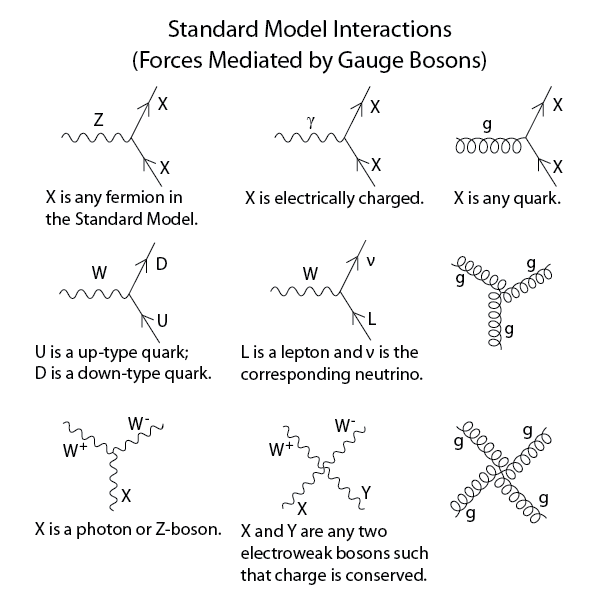
\includegraphics[width=0.7\textwidth]{figures/Phenomenology/Standard_Model_Feynman_Diagram_Vertices.png}
  \caption[Interactions allowed in the SM, excluding those involving the Higgs field]{
    Interactions allowed in the SM, excluding those involving the Higgs field.
    Reproduced from Ref.~\cite{Smith:2646356}.
        }
 \label{fig:SMinteractions}
\end{figure}

The allowed interactions in the SM are illustrated in Fig.~\ref{fig:SMinteractions}. Lines represent
propagating particles, and vertices represent interactions, arising from the
interaction terms in the SM Lagrangian. These illustrations,
known as Feynman diagrams, can be pieced together to give a diagrammatic
picture of a scattering interaction. Fig.~\ref{fig:wz3lfeynman} gives
two illustrative $\cPq\cPq$ interactions---a component of the $\pp$ collision
at the LHC---mediated by the $\PW$ and $\PZ$
bosons, leading to free muons, an electron, and an anti-electron neutrino. 

\begin{figure}[htbp]
  \centering
   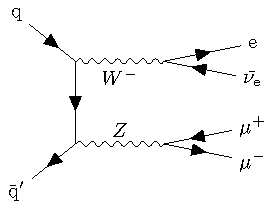
\includegraphics[page=1,width=0.35\textwidth]{figures/FeynmanDiagrams/WZ3lfeynman.pdf}
   \includegraphics[page=2,width=0.35\textwidth]{figures/FeynmanDiagrams/WZ3lfeynman.pdf}
  \caption{
    Feynman diagrams illustrating the $\Pq\Paq\to\mathrm{e}\PAGne\MM$ process,
    proceeding via quark and lepton couplings to the $\PW$ and $\PZ$ bosons.
        }
 \label{fig:wz3lfeynman}
\end{figure}

Feynman diagrams are not just useful as an illustration, they 
represent terms in the perturbative expansion used to model
interactions, specifically, elements of the scattering matrix that 
connects the initial and final state in a scattering experiment. 
So-called Feynman rules
are used to associate the fields and interactions of a diagram with the mathematical
formalism, giving mathematical expressions for the matrix elements
connecting the outgoing particle
four momenta and quantum numbers to the incoming particle properties.
Observables, including the total
rate of production for a final state given the initial state, are dependent
on the square of the scattering matrix elements.

\begin{figure}[htbp]
  \centering
   \includegraphics[page=3,width=0.3\textwidth]{figures/FeynmanDiagrams/WZ3lfeynman.pdf}
   \includegraphics[page=4,width=0.3\textwidth]{figures/FeynmanDiagrams/WZ3lfeynman.pdf}
  \caption{
    Feynman diagrams illustrating the $\Pq\Paq\to\mathrm{e}\PAGne\MM$ process
    with higher-order QCD couplings.
        }
 \label{fig:wz3lfeynmanNLO}
\end{figure}

The diagrams in Fig.~\ref{fig:wz3lfeynman} are not the only possible
set of interactions connecting the $\Pq\Paq$ initial state to the
$\mathrm{e}\PAGne\MM$ state. 
More intricate arrangements of the quark and gluon lines are possible,
as shown in Fig.~\ref{fig:wz3lfeynmanNLO} (left). 
Whereas the diagrams in Fig.~\ref{fig:wz3lfeynman} have four vertices
of fields coupling via the \EW interaction, this diagram has two additional
QCD couplings of the gluon and quarks.
Each vertex contributes and additional factor of the {\EW} or
QCD couplings in the mathematical expression of the scattering matrix element. 
If the coupling term is $\ll$1, the dominant contribution
will come from diagrams such as those shown in Fig.~\ref{fig:wz3lfeynman}, and
it may be possible to neglect the contribution of Fig.~\ref{fig:wz3lfeynmanNLO} (left).
Perturbative calculations rely on this approximation
by restricting a calculation to a maximum ``order'' $\mathcal{O}(\alpha^{n})$ 
in the coupling $\alpha \propto g^2$, by only considering
contributions to a process that have at most a dependence $\alpha^{n}$.

While the diagram in Fig.~\ref{fig:wz3lfeynmanNLO} (right) does lead to a
$\mathrm{e}^{-}\PAGne\MM$ state, it also produces a final-state gluon.
It is tempting to consider this contribution as a separate
process, however, due to the nature of the strong force, such an approach is not favorable experimentally.
Free gluons are not observable, rather, they hadronize into baryons and mesons,
which do not correspond trivially to the radiated partons.
In addition, for gluons radiated at a small angle or low momenta,
it is impossible to experimentally distinguish whether two or one quarks or
gluons are present. For this reason, many leptonic measurements at the LHC
are \emph{inclusive} in the number of associated hadronic particles. That is,
we consider $\pp\to\WZ$ production to include all states producing
the $\mathrm{e}\PAGne\MM$ with any number of associated hadronic objects.

Depending on the process considered and the accuracy needed for a calculation,
neglecting the terms of ``higher order'' may not be appropriate. While the 
Feynman rules are equally applicable for these terms, additional contributions
arise due to the presence of closed loops, as seen for the gluon and quark lines
in Fig.~\ref{fig:wz3lfeynman} (right). These individual diagrams give results
that predict infinite rates, therefore, they cannot correspond to experimental observations.
Fortunately, the situation can be recovered when combining with other diagrams
contributing to the higher-order calculation. A finite contribution can be
isolated and used to describe experimental measurements with incredible accuracy.
Infinite terms remain, but they can be associated with experimentally-established
terms---in particular, the masses and couplings of the theory. This procedure,
known as \emph{renormalization}, is closely connected to the energy scale of the process
and the structure of the fields themselves. In this approach, the coupling constant 
captures the neglected contributions from diagrams contributing at higher perturbative orders,
becoming an effective coupling at the energy scale considered.

\begin{figure}[htbp]
  \centering
   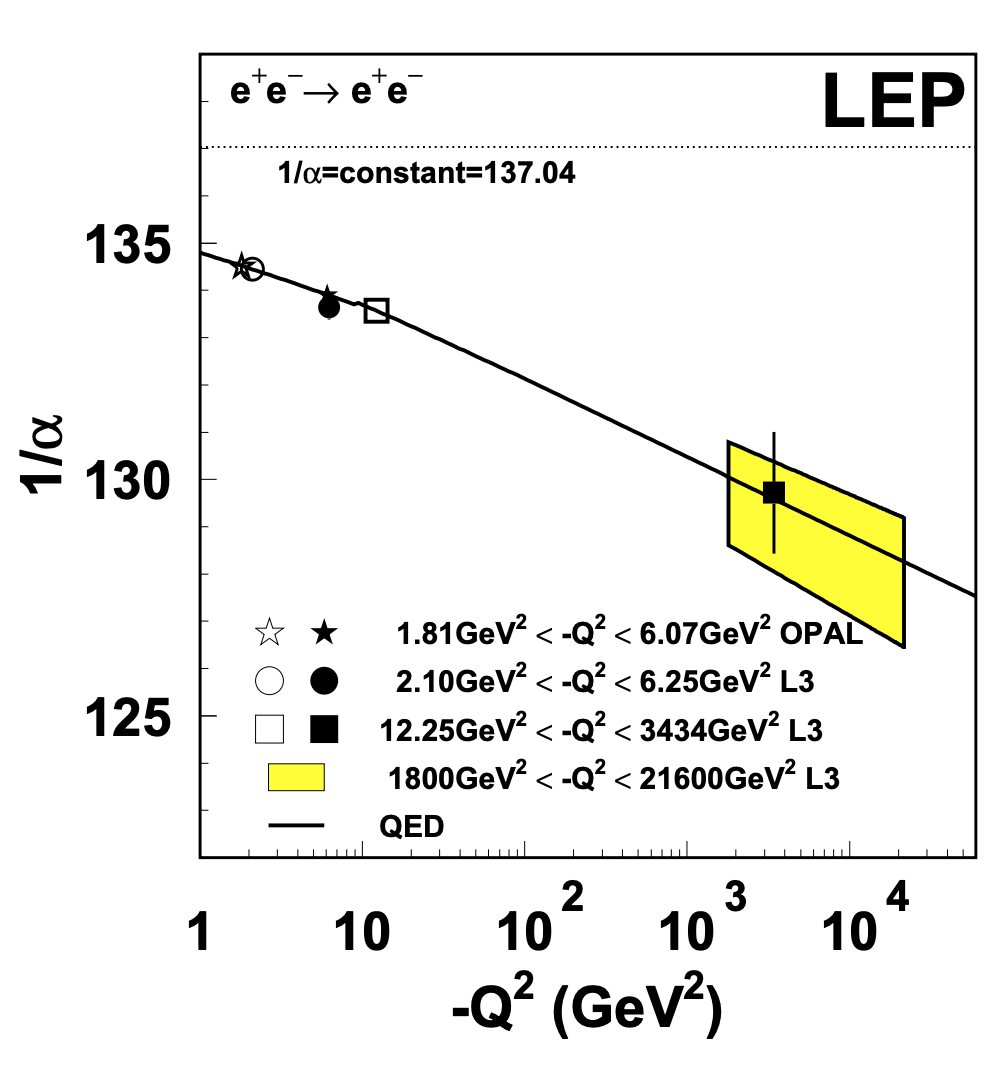
\includegraphics[width=0.39\textwidth]{figures/Phenomenology/alphaRunning.png}
   \raisebox{0.1\height}{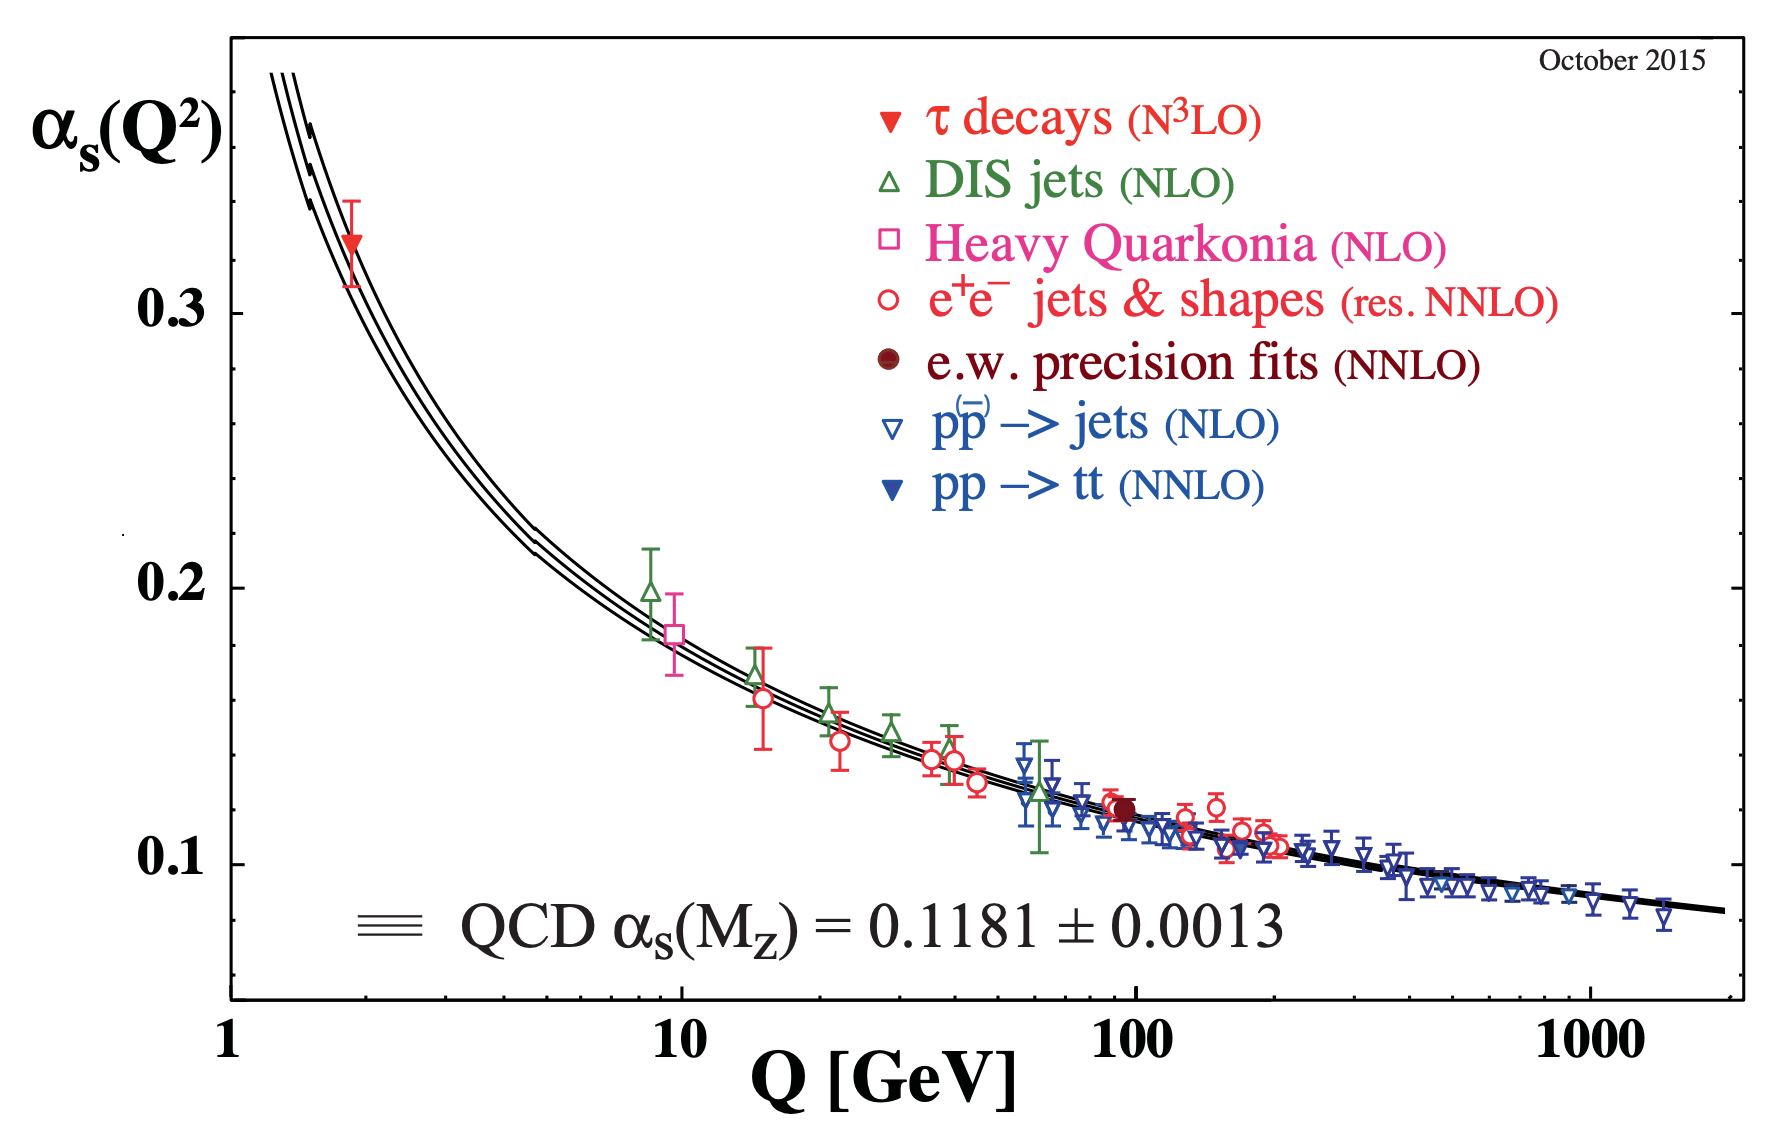
\includegraphics[width=0.59\textwidth]{figures/Phenomenology/alphasRunning.png}}
  \caption[The energy scale dependence of the effective EW and QCD couplings]{
    The energy scale dependence of the effective EW (left, reproduced from Ref.~\cite{Mele:2006ji}) 
    and QCD (right, reproduced from Ref.~\cite{Tanabashi:2018oca}) couplings. The theoretically
    predicted bands and discrete points established experimentally are shown.
  }
  \label{fig:couplings}
\end{figure}

The energy dependence of the effective coupling constants for the 
EW and QCD theories are shown in Fig.~\ref{fig:couplings}.
As shown, the nature of the $\SUthree$ and $\SUtwo$ forces leads to a striking difference
in energy dependence between the two theories: the EW coupling strength increases
with energy, whereas the QCD coupling decreases, leading to the 
confinement of quarks and gluons into bound states, such as the proton and neutron,
at low energies. At the energy scale probed in LHC collisions, the QCD coupling is
sufficiently small for perturbative calculations, however, higher-order corrections
are often significant. The scale dependence of the EW coupling is minimal, so
higher-order EW corrections are often not essential to accurate calculations.
Perturbative calculations are discussed in more detail in Chapter~\ref{ch:simulation}.

\section{The \WZ production at the LHC}

At low energy, the proton can be viewed as a bound state
of the quarks $\cPqu\cPqu\cPqd$. However, at higher energy, the content of the proton
appears more complex. High-energy quarks can radiate gluons, which can split to $\cPq\cPaq$ pairs.
In the high-energy \pp collisions at the LHC, the proton is a source of gluons, and
all flavors of quarks but the heaviest, the top quark.
Therefore, the initial state of fundamental particles in the interactions studied at the LHC is always
composed of quarks and gluons, collectively dubbed ``partons.'' The energy of the colliding 
protons is controlled, but the flavor and energy of the interacting partons can only 
be inferred based on these properties, as discussed in Chapter~\ref{ch:simulation}.

The dominant modes of $\pp\to\WZ\to\threelnu$ 
(were $\ell,\ell'=\mathrm{e},\mu$) production are shown in Fig.~\ref{fig:wz3lfeynman}.
Equivalent diagrams are possible with the $\PW$ and $\PZ$ bosons coupling
to quarks, or the $\PZ$ boson to neutrinos. Many aspects of the processes are similar,
and it is often justified to treat the $\pp\to\WZ$ and $\WZ$ decay to leptons, neutrinos,
or quarks separately. For this reason, we refer to ``$\WZ$ production,'' keeping in mind
that the $\PW$ and $\PZ$ bosons have an extremely short lifetime and are only observable
via their decay products. The results in this thesis exploit the leptonic decay channels,
$\PW^{-}Z\to\EE\mu^{-}\PAGnGm$, 
$\PW^{+}Z\to\EE\mu^{+}\PGnGm$, 
$\PW^{-}Z\to\MM\mathrm{e}^{-}\PGnGm$, and
$\PW^{-}Z\to\MM\mathrm{e}^{+}\PGne$.

Studies of $\WZ$ production at the LHC provide an important test of the SM.
As shown in Fig.~\ref{fig:wz3lfeynman} (right), the process is sensitive to the charged $\PW\PZ\PZ$
coupling, which arises due to the non-Abelian nature of the electroweak
theory, and is exactly predicted in the SM~\cite{Hagiwara:1986vm}. Additional charged
resonances, or other modifications of the \EW sector of the SM, would
modify this process and adjust the rate. Moreover, the process is known
to be sensitive to higher-order corrections~\cite{Grazzini:2016swo}. Measuring this process
with sufficient accuracy to test state-of-the-art calculations, and to 
determine consistency with the SM or uncover hints of new physics, is
of great interest to the LHC experimental program.

As mentioned in the previous section, it is often advantageous to consider
measurements inclusive in the number of hadronic particles. It is possible, however,
to make exclusive measurements, provided that we are careful in how we associate
the number of hadronic objects to the number of partons in a Feynamn diagram.
The solution is to cluster the partons, or hadrons, using algorithms that are
well-behaved for low energy partons. We refer to these clustered hadronic objects as
``jets,'' (\jet) and a close correspondence between experimental measurements and theoretical
predictions has been demonstrated for several so-called jet-clustering algorithms.
The specific algorithms used in this analysis will be discussed in Chapter~\ref{ch:reconstruction}.

The focus of this thesis is the process
$\pp\to\WZjj$, an important subcomponent of the inclusive $\pp\to\WZ$ process
Here, and throughout this thesis, $\WZjj$ refers to $\WZ$ production,
with leptonic decays,
associated with at least two jets in the event, e.g., a final state of $3\ell\nu\jet\jet$.
While it is often useful to relate the $\WZ+2$ partons calculation and the $\WZ+2$ jets (\WZjj)
experimental state, it is important to note that the relationship is most appropriate
when using a common jet clustering algorithm.
The dominant contribution to the $\WZjj$ state is a higher-order correction to the 
diagrams of Fig.~\ref{fig:wz3lfeynman}, where gluons are radiated from the incoming
quarks. Because of the additional
QCD vertices, these diagrams contribute to the \WZjj state at $\mathcal{O}(\alpha_s^{2}\alpha^{2})$,
compared with $\mathcal{O}(\alpha_s^{0}\alpha^{2})$ for the dominant contributions to the $\pp\to\WZ$
process. At this order, contributions from $\cPq\cPg$ and $\cPg\cPg$ initial
states also contribute, slightly enhancing the total $\WZjj$ production rate.

\begin{figure}[htbp]
  \centering
   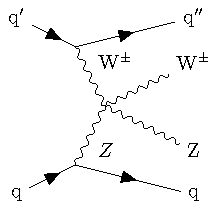
\includegraphics[page=1,width=0.23\textwidth]{figures/FeynmanDiagrams/feynmanEW.pdf}
   \includegraphics[page=2,width=0.23\textwidth]{figures/FeynmanDiagrams/feynmanEW.pdf}
   \includegraphics[page=4,width=0.23\textwidth]{figures/FeynmanDiagrams/feynmanEW.pdf}
   \includegraphics[page=3,width=0.23\textwidth]{figures/FeynmanDiagrams/feynmanEW.pdf}
  \caption[Representative Feynman diagrams for \EWWZ production in the SM]{
    Representative Feynman diagrams for \EWWZ production in the SM,
  including those with quartic \WWZZ interactions (left) and via scattering with the Higgs boson (right).
  }
 \label{fig:feynmanDiagramsVBS}
\end{figure}

Another contribution at $\mathcal{O}(\alpha_s^{0})$ emerges, of
order $\mathcal{O}(\alpha_s^{4})$. 
The subclass of processes with only EW couplings at tree level has a rich
and important phenomenology.
It includes contributions from vector boson scattering (VBS), 
where vector bosons are radiated from the incoming quarks before interacting,
as illustrated in Fig.~\ref{fig:feynmanDiagramsVBS}. 
The VBS processes form a distinct experimental signature characterized by 
the $\PW$ and $\PZ$ bosons with two forward, 
high-momentum jets, arising from the hadronization of two quarks. 
The previously discussed contributions to the \WZjj state that proceed via QCD 
radiation of partons from are referred to as QCD-induced WZjj production (or \QCDWZ).

\section{Probing the electroweak sector through vector boson scattering}

As illustrated in Fig.~\ref{fig:feynmanDiagramsVBS} (right), \EWWZ production 
is sensitive to the quartic couplings of the vector bosons, as well as the 
interactions of the vector bosons and the Higgs boson. Additional interactions
in the \EW sector, such as heavy new scalar Higgs bosons, would lead to additional
contributions, modifying the effective rate of production of \EWWZ events.

The existence of the Higgs boson has strong implications for VBS VV production.
The longitudinally polarized component of the diagrams of Fig.~\ref{fig:feynmanDiagramsVBS} 
that do not involve the Higgs
couplings increase with the scattering energy without bound.
In 1987, an analysis of VBS production of $\PW{+}\PW^{-}$ in $\pp$ collisions
by Lee, Quigg, and Thacker demonstrated that the presence of a scalar boson is necessary to regulate
this component to a finite rate~\cite{Lee:1977yc}.
By analyzing the partial wave amplitudes of the process, they derived a unitary
bound on for the process that stipulated $m_{\PH} \lessapprox 1\TeV$, providing a convincing argument for
the Higgs boson to be discovered at the future LHC. 
While the observed SM Higgs is sufficient to regulate the process, further modifications
could disturb this cancellation, leading to large deviations from the SM predictions.

This thesis presents a measurement of the \EWWZ process under the assumption that
its rate and characteristics are those of the SM prediction. 
We also search for deviations from the SM in both the rate of production of events characteristic
of the \EWWZ process, and in differential distributions sensitive to the scattering energy
of the interaction and the mass of new scalar particles. We interpret the results in terms 
of both explicit models predicting charged Higgs bosons, shown in Fig.~\ref{fig:feynmanNP} (left),
and in the generalized framework of dimension-8 effective field theory, illustrated in
Fig.~\ref{fig:feynmanNP} (right). In this diagram a set of unknown interactions are represented,
which result in a modification of the effective quartic vertices. The charged Higgs 
and EFT models we investigate are complimentary: the former is applicable in a regime
where the collision energy allows the resonant Higgs to be directly produced, whereas
the latter is meaningful when the scale of new physics exceeds the LHC collision energy.
The models we consider are described in more detail in the following sections.

\begin{figure}[htbp]
  \centering
   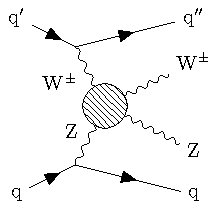
\includegraphics[page=1,width=0.35\textwidth]{figures/FeynmanDiagrams/feynmanNP.pdf}
   \includegraphics[page=2,width=0.35\textwidth]{figures/FeynmanDiagrams/feynmanNP.pdf}
  \caption[Feynman diagrams illustrating hypothetical new physics in the \EWWZ process]{
    Feynman diagrams illustrating hypothetical new physics in the \EWWZ process.
    Charged Higgs production (left) is predicted in many BSM extensions. The aQGC
    approach (right) can be used to parameterize a large class of new interactions modifying the
    \WWZZ process.
        }
 \label{fig:feynmanNP}
\end{figure}

\subsection{Additional Higgs bosons and the Georgi-Machacek model}

In the SM, EWSB is realized by a single isospin doublet scalar field,
as discussed in Section~\ref{sec:ewsb}.
This field is sufficient to give mass to the $\PW$ and $\cPZ$
bosons, while resulting in a scalar $\PH$ boson consistent with the observed
boson with $m_{\PH} = 125\GeV$.  Given the complexity of the fermion sector
of the SM, it is natural to ask if the universe contains a more complex
structure of scalar fields than the single doublet. 
However, SM extensions by arbitrary $\SUtwo$ scalar fields 
are highly constrained by the parameter $\rho \equiv m_\PW^2/m_\PZ^w\cos^2\theta$,
experimentally established to be very close to 1~\cite{Tanabashi:2018oca}.
For a theory with $n$ scalar multiplets
$\phi_i$, with weak isospin $I_i$, weak hypercharge $Y_i$, and vacuum expectation
value $v_i$, $\rho$ is defined in terms of the quantum numbers of the fields
by the following expression at tree level~\cite{Branco:2011iw}
\begin{equation}
  \rho = \sum_{i = 1}^{n} \frac{I_i(I_i+1) - \frac{1}{4}Y_i^2}
              {\frac{1}{2}Y_i^2 v_i} \,,
  \label{eq:rho}
\end{equation}
Extending the scalar sector of the SM by two rather than one doublet satisfies
this expression. This model, known as the Two-Higgs-doublet model (2HDM), has
been extensively studied, in part because the scalar sector of 
many popular theories of supersymmetry have this form.
The 2HDM gives rise to a heavy Higgs boson, a pseudoscalar Higgs boson, and 
charged Higgs bosons $\PH^{\pm}$ in addition to a light SM-like Higgs boson.
In this model, the $\PH^{\pm}$ bosons coupling strongly to the leptons,
and decays to bosons are strongly suppressed in the mass range probed by the LHC~\cite{Arhrib:2016wpw}.

Alternatively, if the Higgs sector of the SM is extended by scalar $\SUtwo$ triplets,
charged Higgs bosons with tree-level couplings to the $\PW$ and $\PZ$ bosons are 
generated by EWSB.
Higgs triplets appear in left-right symmetric~\cite{Pati:1974yy,Mohapatra:1974gc,},
little Higgs~\cite{ArkaniHamed:2002qy,Chang:2003zn,Chang:2003un}, 
and some supersymmetric models~\cite{Garcia-Pepin:2014yfa,Cort:2013foa}.
A simple extension of the SM with Higgs triplets that satisfies experimental
constraints on $\rho$ was proposed by Georgi and Machecek~\cite{Georgi:1985nv}.
In the Georgi Machacek (GM) model, the Higgs sector is extended by a real 
triplet with $Y=0$ and 
a complex triplet with $Y=2$ in addition to the usual SM doublet ($Y =1$). 
After EWSB, this leads to a rich Higgs sector with intriguing phenomenology.
The Higgs sector of the GM has ten physical states that are organized based
on their transformation properties under the approximate global $\SUtwo$ symmetry
of the scalar fields remaining after EWSB, referred to as custodial symmetry~\cite{Sikivie:1980hm}. There are two singlets,
one of which is associated with the observed Higgs boson, a triplet, and 
a fiveplet ($\PH_5^{++}$, $\PH_5^{+}$, $\PH_5^{0}$, $\PH_5^{-}$, $\PH_5^{--}$) that
is fermiophobic. If the mass of the triplet states is greater than the
mass of the fiveplet, the only production mechanism for $\PH^{\pm}$ at the LHC
is vector boson fusion (VBF, shown in Fig.~\ref{fig:feynmanNP}, left). The production cross section is proportional to the variable
$s_{\PH}^2 \equiv \sin^2{\theta_{\PH}}$, where $\sin{\theta_{\PH}} = 2\sqrt{2}v_{\chi}/v$,
the ratio
of the vacuum expectation value (vev) of the triplet fields to the SM vev. 
The $\WZjj$ state probed in this thesis is well-suited for further probes of this model, 
which is significantly less constrained than those charged Higgs with predominantly
leptonic decays.

\subsection{Generalizing new interactions with effective field theory}

Explicit models of charged Higgs production, such as those
discussed in the previous section, provide a well-motivated set of characteristics
to exploit in searches for deviations from the SM. 
In such a paradigm, expectations
about the underlying structure of the theory allow explicit relationships
between independent measurements to be drawn. 
However, when results favor
the SM to a proposed extension, it may be useful to cast a wider net, in search
of more subtle or more exotic extensions. Furthermore, if the mass scale
of new physics---such as a heavy charged Higgs bosons---exceeds the range 
directly probed by 13\TeV \pp collisions, a broad characterization of a deviation,
or lack thereof, may be more meaningful than sensitivity to a particular model.

Effective field theory (EFT) is well suited for a broad characterization
of new physics at a high energy scale. In EFT, the SM is assumed to describe the
field content of the universe below some scale $\Lambda$. 
Additional fields may exist, but they are only directly accessible (e.g., 
resonant production at a collider) above $\Lambda$. Below this scale,
their effect on the low-energy world can be parameterized in terms of the known
SM field content. These interactions are realized by adding additional terms
to the SM Lagrangian, built from the SM fields, of mass dimension $>$4. In order
to restore calculability of these interactions, a dimensionful coupling must also,
which is proportional to the inverse of the scale $\Lambda$.

The bottom-up approach to EFT described here, in which
new interactions are parameterized in terms of the low-energy field content,
is useful because it is consistent with a top down approach, where the low-energy behavior is extracted
from a known full theory~\cite{Kaplan:2005es}. The most well-known example of this is the Fermi theory
of the weak decay $\mathrm{n}\to\PAp\mathrm{e}^{-}\PAGne$. 
A low energy description, in which the leptons, quarks, and neutrinos couple
directly in a four-fermion interaction was original proposed by Fermi without knowledge
of the underlying theory. 
In the full \EW theory, the interaction between
a $\cPqd$ quark of the neutron and an electron is mediated by the $\PW^{-}$ boson,
through $\cPqd\PW^{-}\cPqu$ and $\mathrm{e}^{-}\PW^{-}\PAGne$ couplings of the EW theory.
Because the momentum exchange $p$ of the interaction is on the MeV scale, whereas 
$m_{\PW} = 80.4\GeV$, the full expression for the interaction can be expanded in 
terms of the ratio $p/M$, to derive an approximate theory valid at low energy
with the effective coupling $G_{F} = \sqrt{s}g^2/8m_{\PW}^2$ of Fermi's theory.
In this sense, the low-energy EFT gives insight gives useful predictions within
its energy regime and provides insight into the nature of the full theory.

In this analysis, we consider a set of dimension-8 EFT operators sensitive
to the quartic interactions of the $\PW$, $\PZ$, and $\gamma$. Because an alternative,
largely historical, approach to parametrizing these interactions involves
directly modifying the coupling terms in the Lagrangian, we refer to this 
as a search for anomalous quartic gauge couplings (aQGC). Similarly, anomalous triple gauge
couplings (aTGC), probed in inclusive $\WZ$ production,
can be parameterized by dimension-6 operators. 

The set of operators considered in this analysis
are shown in Equation~\ref{eq:aqgc}.
\begin{equation}
  \begin{aligned}
    \mathcal{L}_\text{S0} = & \frac{f_\text{S0}}{\Lambda^4} \left[(D_\mu \Phi)^\dagger(D_\nu \Phi)\right]\times\left[(D^\mu \Phi)^\dagger(D^\nu \Phi)\right] \\
    \mathcal{L}_\text{S1} = & \frac{f_\text{S1}}{\Lambda^4} \left[(D_\mu \Phi)^\dagger(D^\mu \Phi)\right]\times\left[(D_\nu \Phi)^\dagger(D^\nu \Phi)\right] \\
    \mathcal{L}_\text{T0} = & \frac{f_\text{T0}}{\Lambda^4} \text{Tr}\left[\hat{W}_{\mu\nu} \hat{W}^{\mu\nu}\right] \times \text{Tr}\left[\hat{W}_{\alpha\beta} \hat{W}^{\alpha\beta}\right] \\
    \mathcal{L}_\text{T1} = & \frac{f_\text{T1}}{\Lambda^4} \text{Tr}\left[\hat{W}_{\alpha\nu} \hat{W}^{\mu\beta}\right] \times \text{Tr}\left[\hat{W}_{\mu\beta} \hat{W}^{\alpha\nu}\right] \\
    \mathcal{L}_\text{T2} = & \frac{f_\text{T2}}{\Lambda^4} \text{Tr}\left[\hat{W}_{\alpha\mu} \hat{W}^{\mu\beta}\right] \times \text{Tr}\left[\hat{W}_{\beta\nu} \hat{W}^{\nu\alpha}\right] \\
    \mathcal{L}_\text{M0} = & \frac{f_\text{M1}}{\Lambda^4} \left[(D_\mu \Phi)^\dagger(D_\nu \Phi)\right]\times\left[(D^\mu \Phi)^\dagger(D^\nu \Phi)\right] \\
    \mathcal{L}_\text{M1} = & \frac{f_\text{M1}}{\Lambda^4} \left[(D_\mu \Phi)^\dagger(D^\mu \Phi)\right]\times\left[(D_\nu \Phi)^\dagger(D^\nu \Phi)\right]
  \end{aligned}
  \label{eq:aqgcOperators}
\end{equation}
Here
\begin{equation}
  \hat{W}_{\mu\nu} = \sum_j W_{\mu\nu}^j \frac{\sigma^j}{2}\,,
\end{equation}
where $W_{\mu\nu}$ are the $\SUtwo_{L}$ fields before EWSB
and the values $f_{\text{S}i}$, $f_{\text{T}i}$, and $f_{\text{M}i}$ are
dimensionless couplings to the dimension-8 operators.

The operators probed are a subset of those outlined in 
Ref.~\cite{Eboli:2006wa}, which proposes
nine independent dimension-eight operators that
assume the $\SUtwo\times\Uone$ symmetry of the EW gauge sector as well as
the presence of an SM Higgs boson. All operators are
charge conjugation and parity conserving.
The $\mathcal{L}_\text{Si}$ operators
are a function of the scalar Higgs field. The $\mathcal{L}_\text{Ti}$ operators are
functions of the gauge fields, and the $\mathcal{L}_\text{Ti}$ operators are
built from a mix of the scalar and gauge fields. The quartic gauge
coupling can be expressed in terms of these operators as 
\begin{equation}
\mathcal{L}_{quartic} = f_\text{S0}\mathcal{L}_\text{S0} + f_\text{S1}\mathcal{L}_\text{S1} \,.
\end{equation}
With $f_\text{S0} = -f_\text{S1} = f$, non-zero values of $f$ give a rescaling
of the SM coupling by $(1+fv^{4}/8)$.

\section{Previous results}

\subsection{Measurements of \WZ production}

The $\WZ$ production was first observed
in $\Pp\PAp$ collisions by the CDF~\cite{Aaltonen:2012vu,Abulencia:2007tu} 
and D0~\cite{Abazov:2012cj} Collaborations at the Tevatron in 2006. 
The inclusive \WZ production cross section in \pp collisions 
has been measured in the leptonic decay modes by the ATLAS and CMS Collaborations 
at 7, 8, and $13\TeV$~\cite{Aad:2012twa,Aad:2016ett,Aaboud:2016yus,Aaboud:2019gxl,Khachatryan:2016tgp,Khachatryan:2016poo}, 
A summary of these measurements is 
shown in Fig.~\ref{fig:WZxsecSqrts}. The summarized experimental results are obtained
by measuring $\pp\to\WZ\to\ell'\ell'\ell\nu$ process, corrected for the 
independently-measured leptonic branching ratios (the percentage of events with
$\PW\to\ell\nu$ and $\PZ\to\ell'\ell'$ to all other decay channels), to obtain a total
rate for the process $\pp\to\WZ$. Theoretical predictions are shown at 
next-to-leading order (NLO) in QCD, in which all contributions to the process 
up to $\alpha^{2}\alpha_s$ are considered in the calculation,
and at next-to-next-to-leading order (NNLO), which considers contributions up 
to $\alpha^{2}\alpha_s^{2}$. The predictions are obtained using the programs
MCFM~\cite{Campbell:2011bn,Campbell:2015qma} and MATRIX~\cite{Grazzini:2016swo,Grazzini:2017mhc}.
The data exhibit a slight preference for the higher-order prediction, demonstrating
the importance of both high-precision measurements and calculations.

\begin{figure}[htbp]
  \centering
   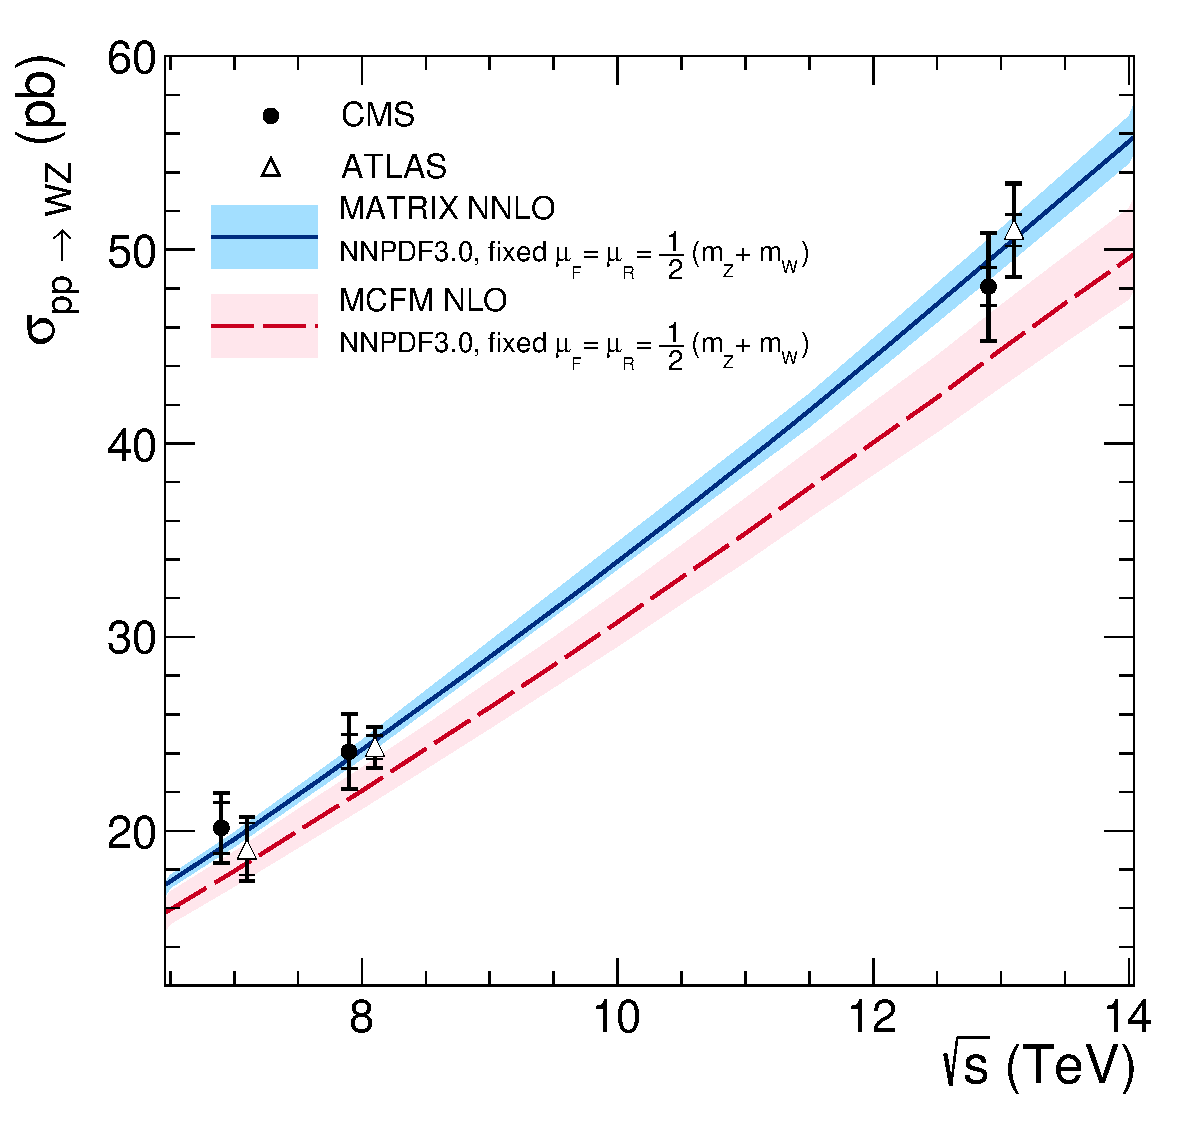
\includegraphics[width=0.8\textwidth]{figures/Phenomenology/WZCrossSection_preliminary_2019-02-23.pdf}
  \caption{
    The measured $\pp\to\WZ$ production cross sections at 7, 8, and 13\TeV compared with
    theoretical predictions at NLO and NNLO in QCD.
        }
 \label{fig:WZxsecSqrts}
\end{figure}


\subsection{Measurements of $\WZjj$ production and electroweak \WZ production}

Fig.~\ref{fig:WZnJets} shows the distribution of the number of jets associated with
the selected $\ell\ell\ell'\nu$ state in data collected by the CMS experiment
in 2015. This analysis, the first measurement of the $\WZ$ process at 13\TeV,
was a critical first step towards the $\WZjj$
studies presented in this thesis. The expected contribution from the $\WZ$
process, along with the estimated backgrounds, are seen to be in good agreement
with the observed data. This studies of this thesis are performed with
a higher-luminosity data set, in order to exploit the kinematics variables of the selected
jets to isolate the $\EWWZ$ and new physics contributions.

\begin{figure}[htbp]
  \centering
   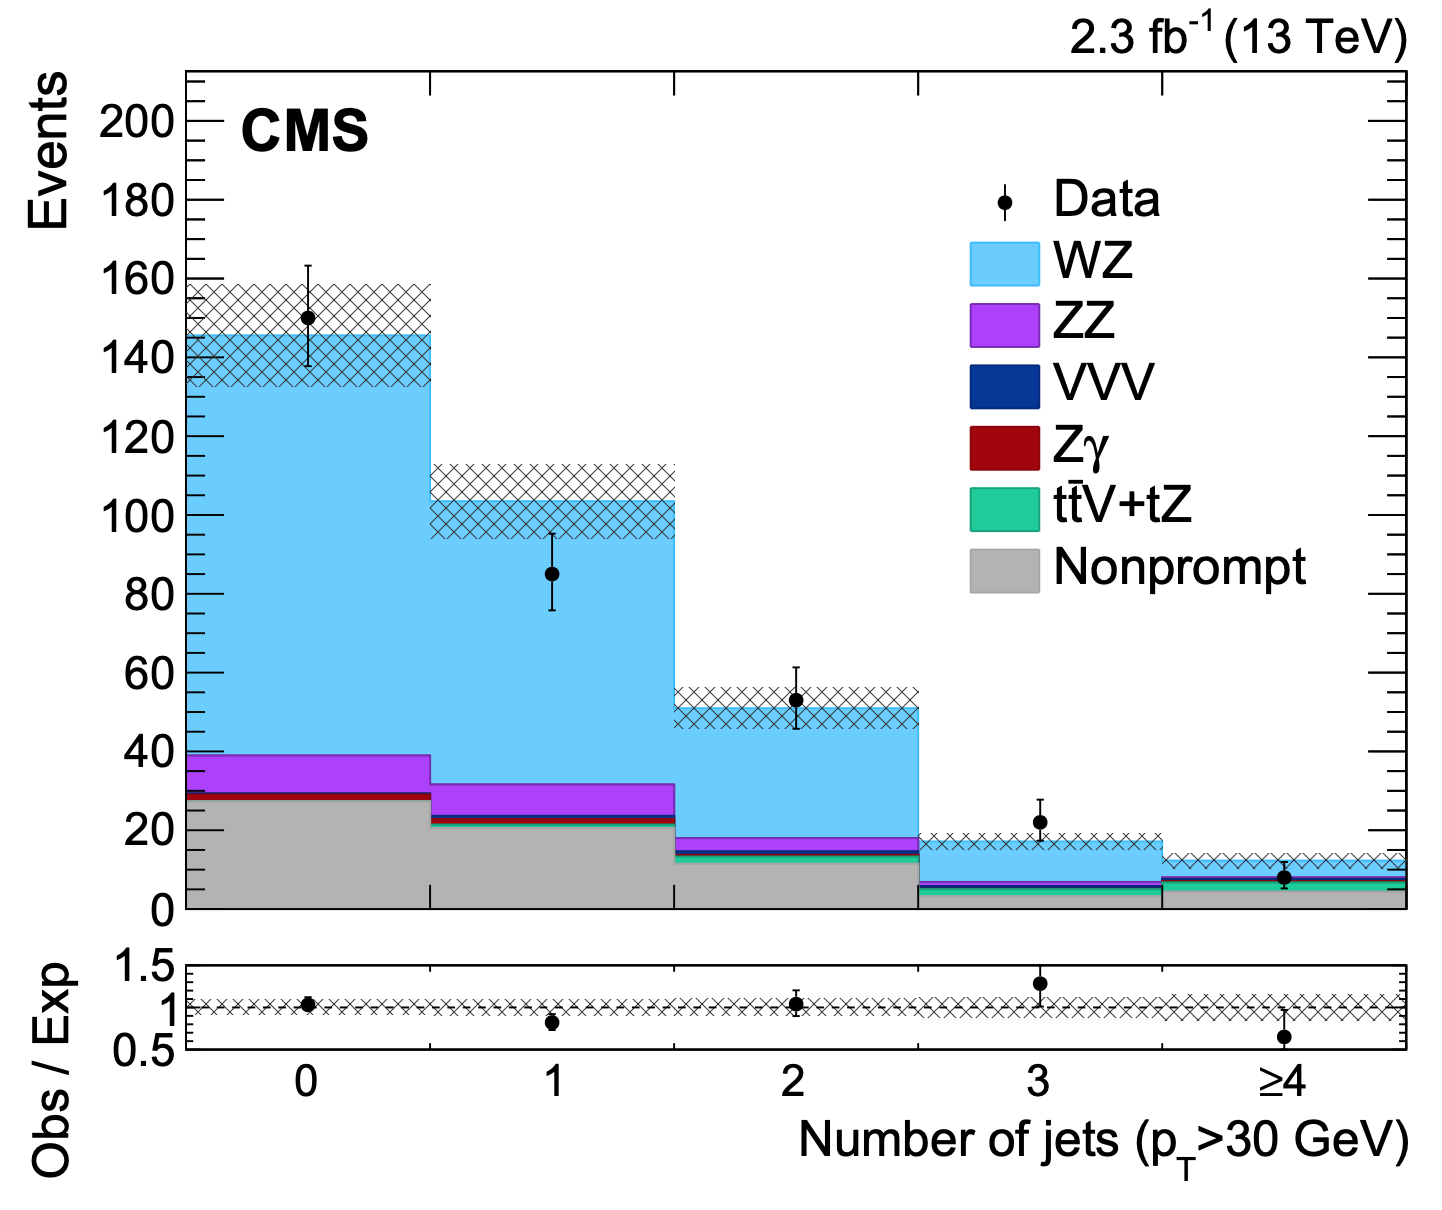
\includegraphics[width=0.6\textwidth]{figures/Phenomenology/WZnJets2015.png}
  \caption{
    The number of jets in selected $\ell'\ell'\ell\nu$ events
    for the observed data and the expected $\WZ$ signal and background 
    contributions using 2.3\fbinv of data collected by the CMS experiment in
    2015~\cite{Khachatryan:2016tgp}.
        }
 \label{fig:WZnJets}
\end{figure}

The first studies of VBS production of pairs of massive vector 
bosons---termed diboson production, or VV production, where $\text{V}=\PW,\PZ$---were 
performed using in the $\pp\to\Wpm\Wpm\to\ell^{\pm}\nu\ell'^{\pm}\nu'$
channel at 8\TeV~\cite{Khachatryan:2014sta,Aad:2014zda,Aaboud:2016ffv}.
This channel is advantageous at the LHC, because, contrary to all other VV states,
the {\EW}-induced production dominates the QCD-induced production. The first
measurement of VBS production of a massive VV state with statistical significance
exceeding 3.0 standard deviations ($\sigma$) is presented by the ATLAS Collaboration 
in the analysis of Ref.~\cite{Aad:2014zda}.
The \EWWZ production was also studied at 8\TeV by the ATLAS Collaboration,
which places upper limits on the production cross section in Ref.~\cite{Aad:2016ett},
and the CMS Collaboration, which reports a \WZjj cross section in a region
sensitive to \EWWZ production in Ref.~\cite{Khachatryan:2014sta}.

Studies of \EW $\Wpm\Wpm$ have recently been performed by the CMS and ATLAS Collaborations at 
13\TeV~\cite{Sirunyan:2017ret,ATLAS-CONF-2018-030}.
The first measurement of \EW VV production with a statistical significance greater than 5 standard 
deviations, considered the standard for discovery of new processes by the experimental particle 
physics community, is presented by the CMS Collaboration in Ref.~\cite{Sirunyan:2017fvv}. A subsequent study
performed by the ATLAS Collaboration~\cite{ATLAS-CONF-2018-030} reports a comparable observation for the process.
The first study of the \EW VV production with a $\PZ$ boson was performed in the $\pp\to\ZZ$ channel
by the CMS Collaboration~\cite{Sirunyan:2017jej}. The observed statistical significance of the 
measurement is $2.7\sigma$ with $1.9\sigma$ expected in the SM.

The analysis of this thesis, submitted for publication to the journal \emph{Physics Letters B}~\cite{Sirunyan:2019ksz},
is the first study of \EWWZ production performed by the CMS.
An analysis using a comparable data set of $\pp$ collisions at 13\TeV
has also been submitted to the journal \emph{Physics Letters B} by the ATLAS collaboration~\cite{Aaboud:2018ddq}.
The ATLAS analysis reports and observation of the \EWWZ process with observed statistical significance of
$5.3\sigma$, with $3.4\sigma$ expected in the SM.


\subsection{Searches for anomalous quartic gauge couplings}

Anomalous triple and quartic gauge couplings were studied with
measurements of $\PW\PW$ and $\PW\PW\gamma$ production in electron-positron collisions
at the LEP Collider at CERN by the ALEPH, DELPHI, L3, and OPAL Collaborations~\cite{LEP-2}.
These processes are sensitive to the triple vector boson couplings
$\WWZ$ and $\PW\PW\gamma$, and the quartic couplings $\PW\PW\gamma\gamma$
and $\PW\PW\PZ\gamma$. The production rate and angular distributions of the decay
products of the vector bosons in these states were used to derive values 
of the triple and quartic couplings. No deviations were observed from the 
predictions of the SM were observed.
Limits on the anomalous triple gauge coupling \WWZ~\cite{Hagiwara:1989mx} 
were also presented by CDF and D0 collaboration in 
Ref.~\cite{Aaltonen:2012vu,Abazov:2012ze}, followed by studies performed by the ATLAS and CMS Collaborations in 
Refs.~\cite{Aad:2016ett,Khachatryan:2016poo}. 

Experimental sensitivity to the quartic coupling \WWZZ 
was first achieved at the LHC.
In pp collisions, quartic WZ interactions are accessible through 
VBS \VV production or trough triple vector boson production (\VVV).
Constraints on the deviations of quartic couplings from the SM prediction in
WZ events with at least two jets were first
presented by the ATLAS collaboration at 8 TeV~\cite{Aad:2016ett}. This thesis
reports the first study of aQGCs in the \WZ channel at 13\TeV.

\begin{figure}[htbp]
  \centering
   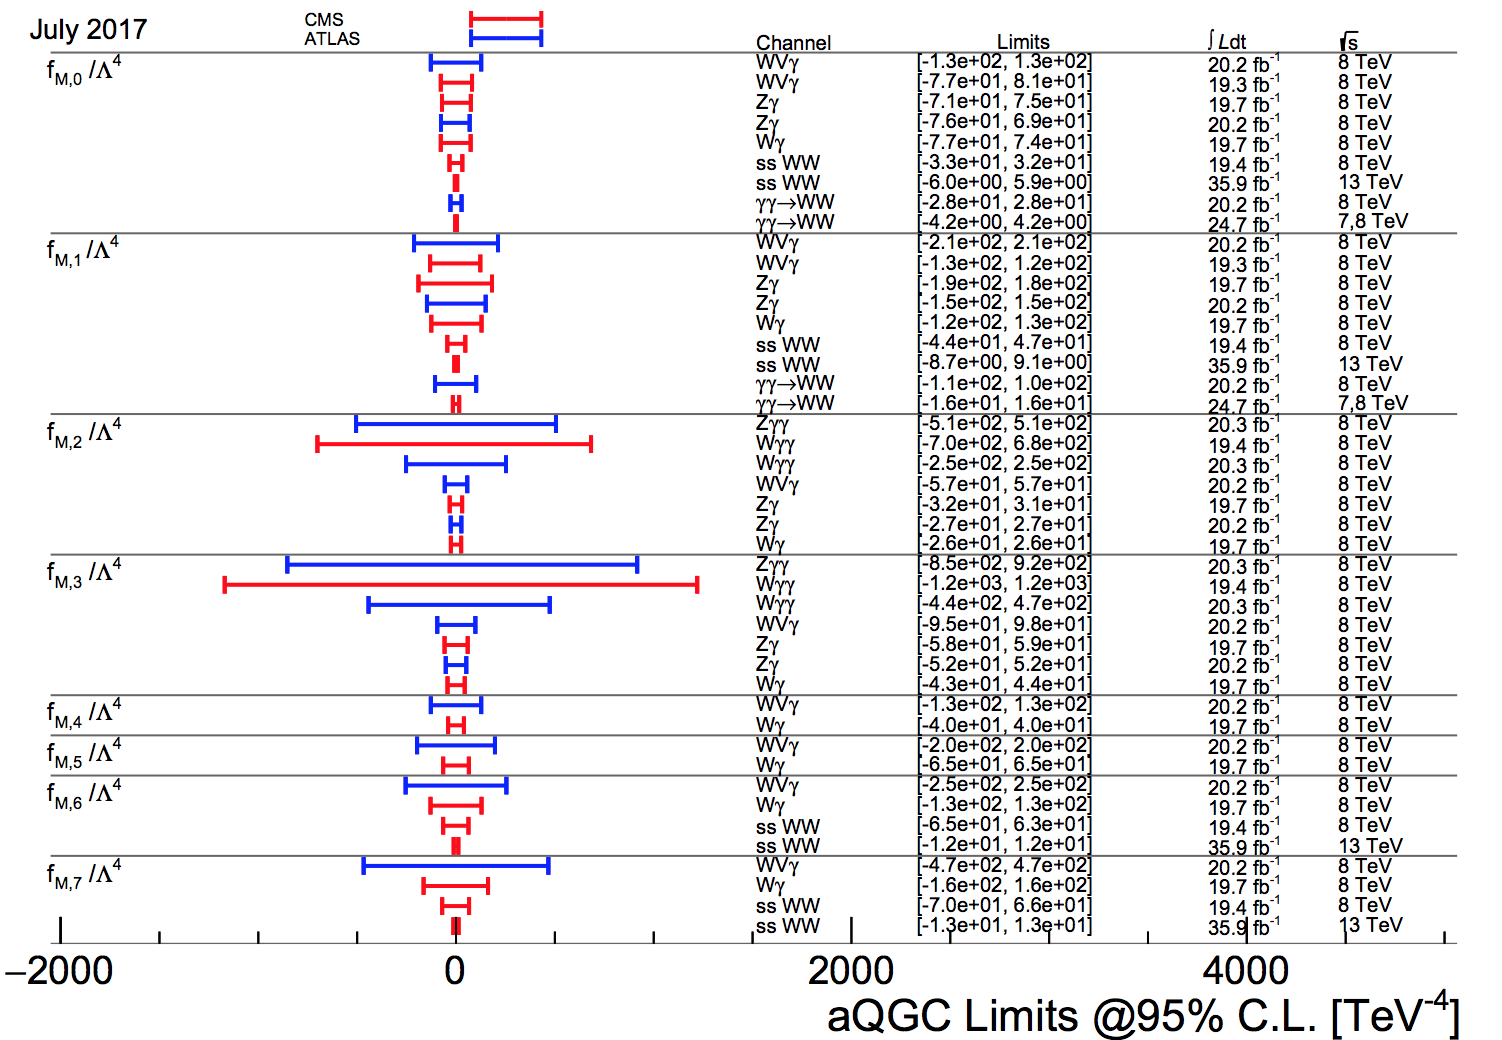
\includegraphics[width=0.95\textwidth]{figures/Phenomenology/FM0_limits_Jun2017.png}
  \caption{
    Constraints on the parameters f$_{\text{Mi}}/\Lambda^4$ for dimension-8 EFT
    operators from the CMS and ATLAS experiments.
        }
 \label{fig:aQGCs}
\end{figure}

Fig.~\ref{fig:aQGCs} illustrates the constraints on the operator parameters
and scale of new physics for the dimension-8 quartic operators
$\mathcal{L}_{\text{T}i}$ from previous studies by the ATLAS and CMS Collaborations.
The most sensitive measurements are those performed in the $\Wpm\Wpm$ channel
reported in Ref.~\cite{Sirunyan:2017ret} and in the $\ZZ$ channel, reported in Ref.~\cite{Sirunyan:2017jej}.

\subsection{Searches for charged Higgs production via vector boson fusion}

The first studies of the production of charged Higgs bosons produced via VBF
and decaying to $\WZ$ at the LHC were performed by the ATLAS Collaboration
at 8~\TeV~\cite{Aad:2015nfa}. The analysis exploited the decay channel
$\Wpm\to\cPq\cPaq'$, $\PZ\to\ell\ell$ 
to place the first direct production constraints on the GM model, as well as model-independent
limits on the production of a narrow-width charged Higgs produced via VBF.
The CMS Collaboration performed the first study of the VBF $\PH^{\pm}$ 
exploiting the leptonic decay channel $\WZ\to\ell\ell\ell'\nu$,
using $15.2\fbinv$ of data collected at $13\TeV$~\cite{Sirunyan:2017sbn}.
The ATLAS Collaboration recently performed an analysis of the same channel
using the data delivered by the LHC in 2016, corresponding to $36.1\fbinv$~\cite{Aaboud:2018ohp},
extending the constraints of the previous CMS analysis.
A local excess of events over the SM prediction at a resonance mass of
around 450\GeV was suggested by this analysis, with a global significance
of $1.9\sigma$ when interpreted in the GM model.
The analysis presented in this thesis extends the results of the previous CMS study, 
and is comparable to the recent study by the ATLAS Collaboration.

\begin{figure}[htbp]
  \centering
   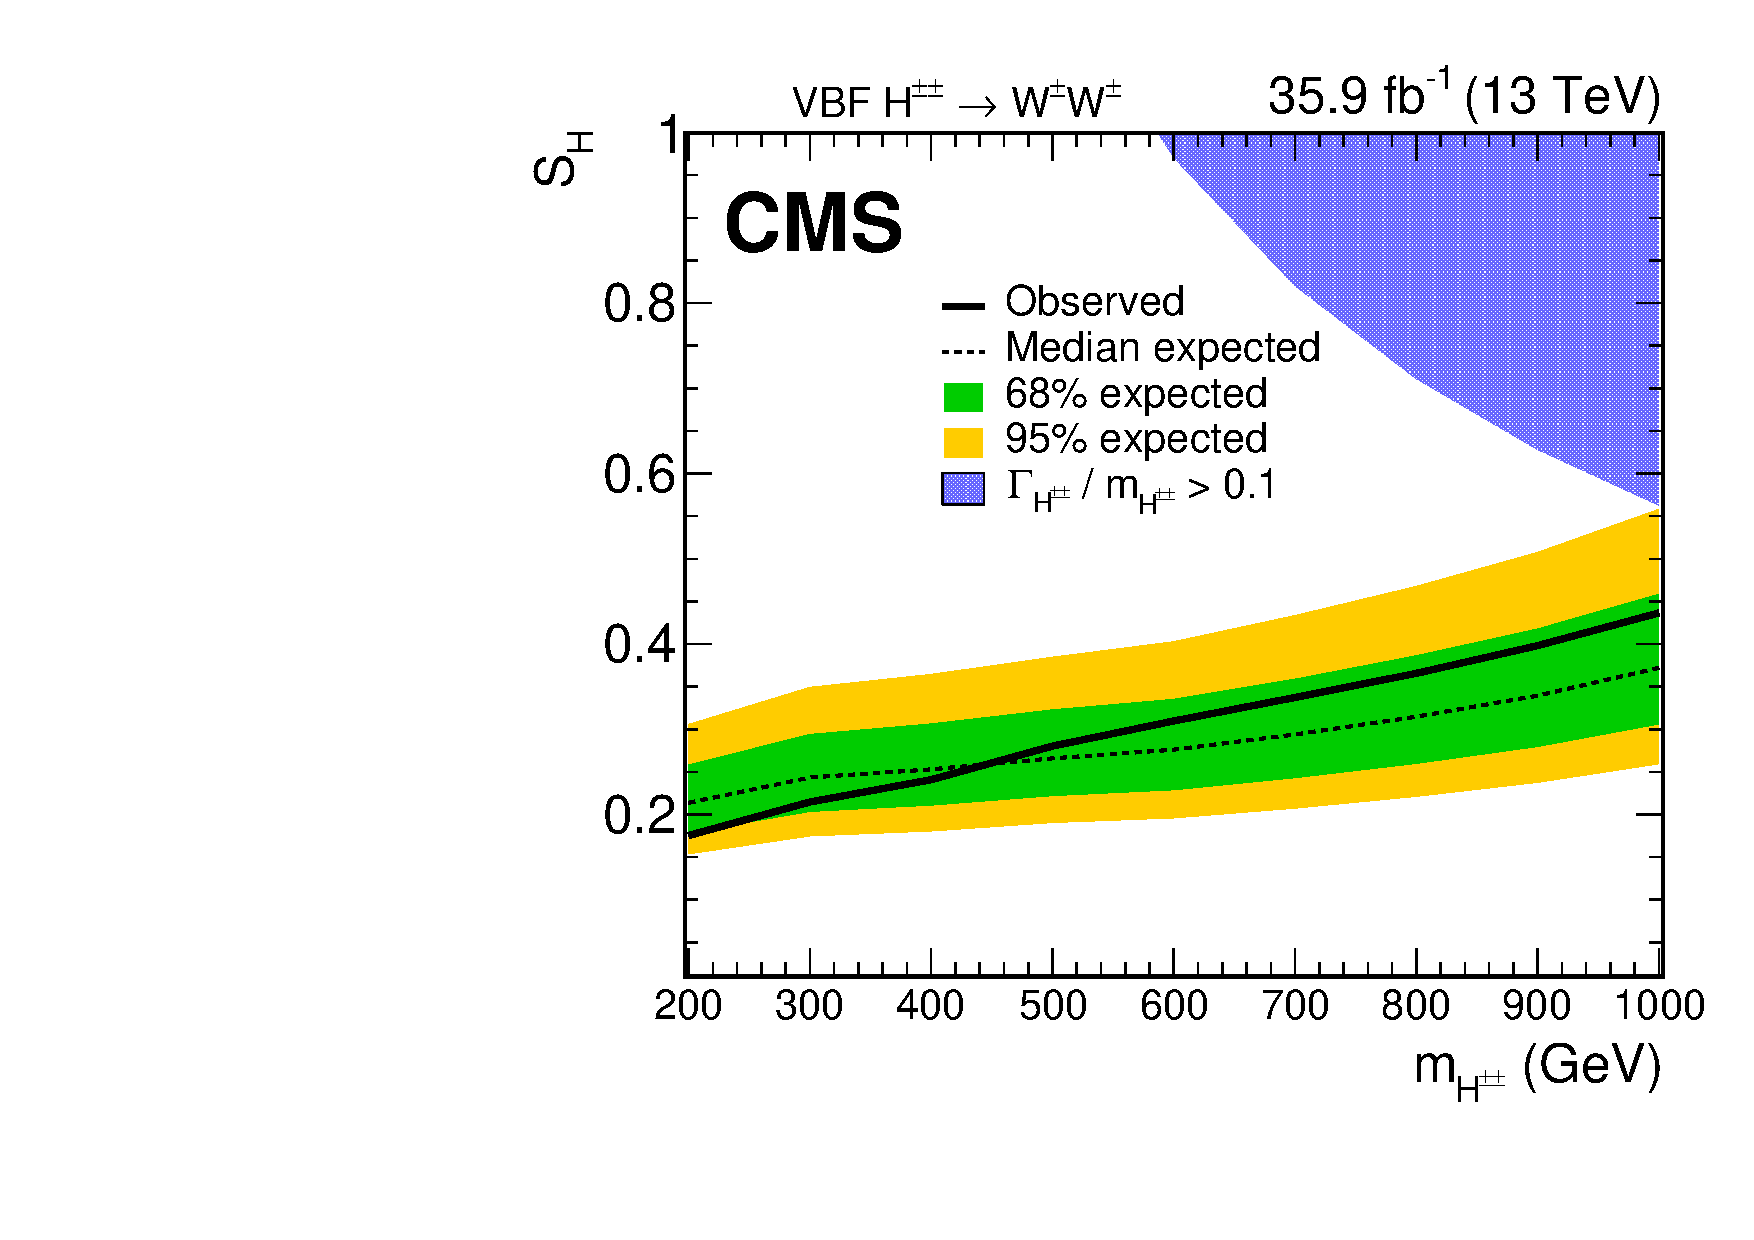
\includegraphics[width=0.44\textwidth]{figures/Phenomenology/CMS-SMP-17-004_Figure_003-b.pdf}
   \raisebox{0.08\height}{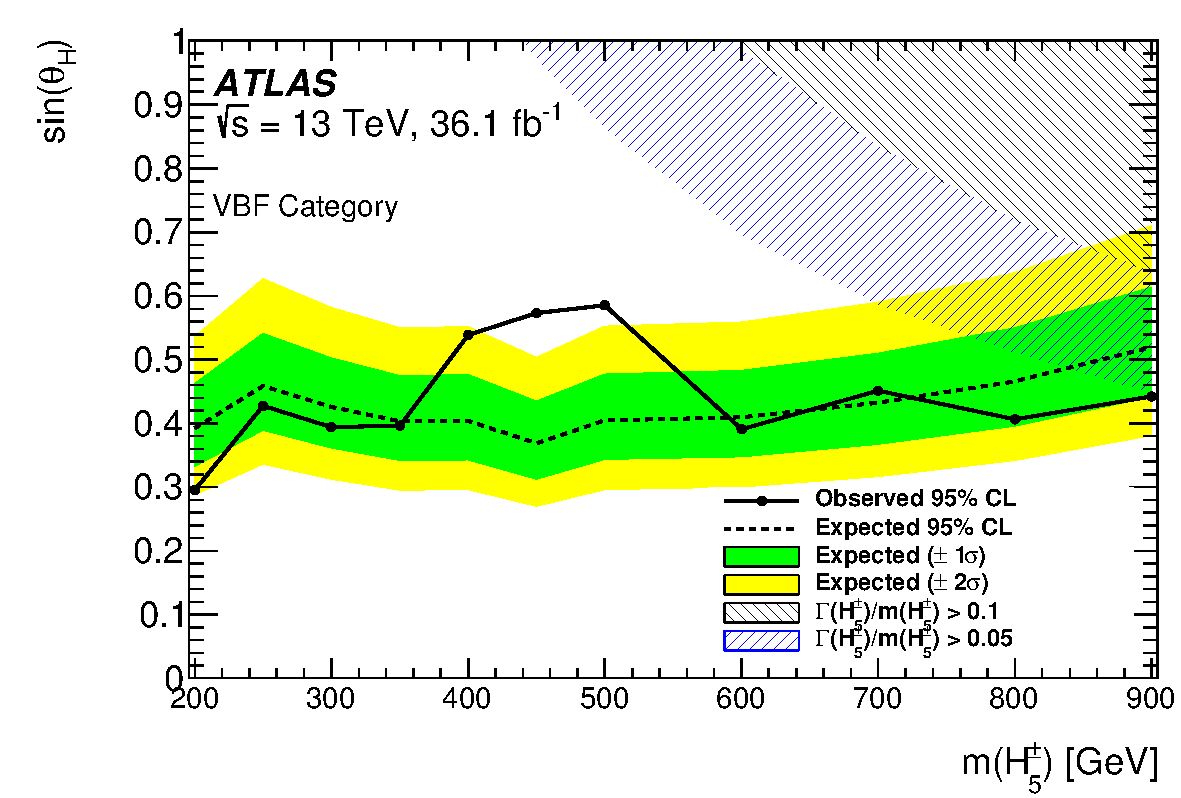
\includegraphics[width=0.54\textwidth]{figures/Phenomenology/ATLAS-EXOT-2016-11_fig_07b.pdf}}
  \caption{
    Limits on production of doubly charged (left, from Ref.~\cite{Sirunyan:2017ret}) 
    and charged Higgs bosons (right, from Ref.~\cite{Aaboud:2018ohp}) in the H5plane defined by the GM model.
        }
 \label{fig:GeorgiMachacekLimits}
\end{figure}

Members of the custodial fiveplet in the GM model have a common mass $m_{\PH^{5}}$.
Therefore, limits on doubly charged Higgs bosons $\PH^{\pm\pm}$
are complementary to those obtained for $\PH^{\pm}$ production when interpreted under this model. 
The ATLAS and CMS
Collaborations have studied $\PH^{\pm\pm}$ production with decays to same-sign
$\PW$ bosons at 8\TeV~\cite{Aad:2014zda,Khachatryan:2014sta}, and the CMS Collaboration has presented
constraints at 13\TeV~\cite{Sirunyan:2017ret}. 
The constraints on the VBF production of $\PH^{\pm}$ in the GM model from Ref.~\cite{Aaboud:2018ohp}
and for $\PH^{\pm\pm}$ from Ref.~\cite{Sirunyan:2017ret} are shown in Fig.~\ref{fig:GeorgiMachacekLimits}.
The limits are presented in terms of $s_{\PH}^2$ and the mass of the $\PH^{\pm}$ or $\PH^{\pm\pm}$
boson, which defines the ``H5plane'' proposed by the LHC Higgs Cross Sections Working Group in Ref.~\cite{deFlorian:2016spz}.
The H5plane is defined with the assumptions that the triplet mass is greater than the 
fiveplet mass and that the parameters of the model allow perturbative calculations. 
Additional constraints on the GM model arise from studies of $\cPqb$ hadron decay
and heavy Higgs boson searches, which are impacted by contributions from additional
Higgs bosons contributing in loop diagrams, but these constraints are exceeded
by the direct measurements discussed here. Global fits of the direct and indirect
constraints on the GM model can be found in Ref.~\cite{Chiang:2018cgb}.

\section{Motivation and content of this result}
The work presented in this thesis
has two related motivations: performing a measurement of a rare
process predicted by the SM, and searching for signs of 
BSM physics in a channel and topology sensitive to modifications of
the EW sector of the SM.
Characterizing the self-interactions of the vector bosons is an important
step to understanding the self-consistency of the SM, and a useful probe
of possible deviations from its predictions. Because the production of events
with multiple vector bosons in the final state
requires collisions with a high center of mass energy, the LHC has
the potential to explore these states in more depth 
than previously achieved.

We perform complementary interpretations of the
observed data and its consistency with the prediction of the SM or signs 
of new physics. In particular, we measure

\begin{itemize}
  \item The total production rate of $\PW\PZ\jet\jet \rightarrow 3\ell\nu\jet\jet$ in
    fiducial regions with enhanced contributions from \EWWZ production
  \item The consistency of the \EWWZ production rate
    with the SM prediction and the statistical significance at which this rate
    can be established as non-zero.
\end{itemize}

We also place constraints on hypothetical new physics using the kinematic
distributions of selected \WZjj events with a VBS topology. 
These processes would be characterized by and excess of VBS \WZ events
with high $m_{\WZ}$, due to the modifications of the quartic VVVV interaction
in a manner sensitive to the scattering energy.
We place limits on the production and model parameters of

\begin{itemize}
  \item Charged Higgs bosons, in a model-independent manner (assuming
    a small $\PH^{\pm}$ width) and in the Georgi-Machacek model.
  \item Anomalous quartic gauge couplings, using the language of
    dimension-eight effective field theory.
\end{itemize}

\chapter{The CMS Experiment at the CERN LHC}

The Large Hadron Collider (LHC) at the European Organization for Nuclear Research (CERN)
is the world's largest and most powerful particle collider.~\cite{Evans:2008zzb} It collides protons 
at a center of mass energy of $13\TeV$, and lead ions at $2.76\TeV$ per nucleon.
Collisions of protons at the LHC are the sole focus of this thesis. 
The protons or ions are brought to collision at the center of four large detectors,
themselves a combination of many detector technologies. 
The particle detectors at the LHC were conceived, developed, and constructed over decades
by collaborations of thousands of scientists from hundreds of nations to
achieve a broad program of research. The detectors were designed and are operator 
by mutually exclusive collaborations of scientists working independently,

The detector sites are

\begin{itemize}
  \item A Large Ion Collider Experiment (ALICE) detector, located at access point 2.
  Designed for the study of lead-ion collisions, especially for the characterization
    of quark gluon plasmas formed in collisions.~\cite{Aamodt:2008zz}
  \item A Large Toroidal LHC ApparatuS (ATLAS) detector, located at access point 1.
  A general purpose detector. Designed for sensitivity to new physics
  with decays to stable SM particles, in particular the 
    discovery and characterization of the SM Higgs boson.~\cite{Aad:2008zzm}
  \item The Compact Muon Solenoid (CMS) detector, located at access point 5.
    A general purpose detector with comparable measurement potential to the ATLAS detector.~\cite{Chatrchyan:2008aa}
  \item The Large Hadron Collider Beauty (LHCb) detector, located at access point 8.
  Designed to characterize the production and decay of b-quark hadrons. Particularly
    focused on CP violation in these decays.~\cite{Alves:2008zz}
\end{itemize}

Results in this thesis are based on an analysis of proton--proton collisions at the LHC 
collected by the CMS detector in 2016. This chapter describes the design principles of the 
LHC and the CMS detector, as well as their operating characteristics in 2016.
  
\section{The Large Hadron Collider}
The LHC was proposed to the CERN council, the management group of the 
laboratory, in 1994, and accepted
with a preliminary budget in 1995. Construction was initially completed in
2008, with full operation beginning in 2009 after setbacks 
encountered in the initial commissioning.
The collider is located on the outskirts
of Geneva, Switzerland and in the nearby French countryside,
which has been the site of the CERN laboratory since it was founded in 1954.
The project was funded by the 20 member states of CERN, as well
as monetary and research contributions from many other nations participating 
in the project, including the United States.

The principle design considerations of a particle collider are the energy
of the particle collisions, the rate of collisions, and the objects collided.
The collided objects determine the possible interactions which can be probed,
while the energy of the collision drives the mass range which can be probed,
given that the produced particle mass $m$ be less than the 
center of mass energy. As particle interactions are quantum mechanical 
and fundamentally stochastic in nature, the rate of collisions is also 
critical for achieving statistically significant measurements.

Several characteristics of proton--proton collisions motivated the decision 
to use protons in the world's highest-energy collisions. Existing high-energy
accelerators, notably the Large Electron Positron Collider (LEP) collider
at CERN and the Tevatron collider at Fermilab in the United States, collided
particle--antiparticle pairs. This is advantageous for processes which proceed by annihilation, 
but requires production of positrons or antiprotons, which is a significantly
bottleneck on achieving a high rate of collisions. 

The LHC is situated in a $26.7\unit{km}$ tunnel, $45$--$170\unit{m}$
below the Swiss and French country side. The tunnel pre-dates the LHC,
having been originally built for the Large Electron Positron (LEP) collider.
It consists of 8 straight sections $528\unit{m}$ in length, and 8 arced sections.
The majority of the tunnel is $3.7\unit{m}$ in diameter, with larger excavated
areas at the four experimental caverns and other access points.
The primary motivation for an underground tunnel is to circumvent the high
cost of land acquisition, but underground operation is also advantageous for
reducing the cosmic radiation reaching the experimental cavern and  
for shielding the radiation produced by the LHC.

The protons are directed through pipes inside the tunnel, which are held
at high vacuum. The positions and accelerations of the protons are controlled 
by magnetic and electric fields maintained by instrumentation surrounding the 
vacuum pipes. The arced sections are equipped with dipole magnets,
which direct charged objects along a circular path.
The size of the LEP tunnel prohibited the installation of two independent beam
systems, which led to the adoption of a unique "two-in-one" superconducting
magnet design~\cite{}, shown in Fig~\ref{fig:dipoleXsec}. 

\begin{figure}[htbp]
  \centering
   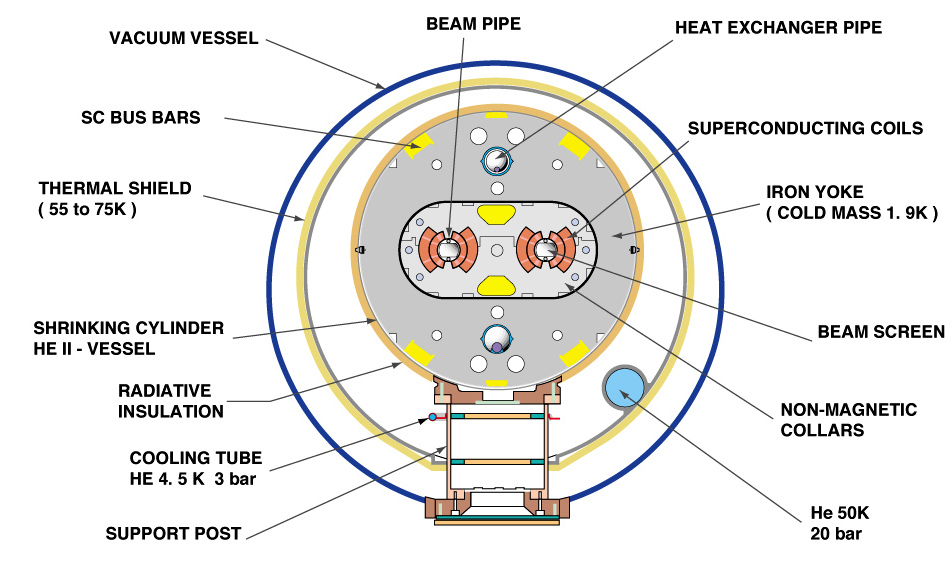
\includegraphics[width=\textwidth]{figures/LHCandCMS/dipoleXSec.jpeg}
  \caption{
    Cross section of an LHC dipole magnet~\cite{Jean-Luc:841539}.
        }
 \label{fig:dipoleXsec}
\end{figure}

Neglecting synchrotron radiation,
the primary limitations on the energy of a synchrotron come
from the magnetic field of the bending magnets and the radius of curvature
of the tunnel. For an particle of charge $q$ with velocity $v$ accelerated at
in a circular 
trajectory of radius $R$ trough a magnetic field of strength $B$
The energy $E$ of the particle is given by

\begin{equation}
  E = eBRv \approx qBRc \,,
\label{eq:beamEnergy}
\end{equation}

where $v \approx c$, the speed of light, for $p \gg m$. Increasing the radius
requires a larger tunnel, which is limited by the cost of construction. 
The LHC tunnel size was set by the existing LEP tunnel, so achieving
a sufficient magnetic field was a major focus of the LHC development. 

Dipole magnets with a maximum field strength of $8.33\unit{T}$ were achieved
at an affordable cost through major technological advances. Such a high 
field necessitates the use of superconducting magnets. The magnets 
are constructed of niobium-titanium, and are operated at $1.9\unit{K}$,
lower than any previous accelerator. 
at 
first accelerator to operate 
In particular,
the LHC is the first accelerator to operate 
Because about 80\% of the arced sectors of the LHC are equipped with dipole magnets,
the bending radius of the dipoles is $2.804\unit{km}$, yielding the design energy
of $7\TeV$ per beam from Equation~\ref{eq:beamEnergy}.

Also brief mention of the 

How it accelerates protons (e.g., the system of accelerators)

The magnet design and characteristics 

The RF and bunch characteristics

Focusing beams to collisions


\section{Operation of the LHC in 2016}
\section{The Compact Muon Solenoid experiment}

The CMS detector is a general-purpose detector designed to 
study particle production and interactions at the TeV scale.
A major design principle of the CMS detector was the ability to 
probe the nature of electroweak symmetry breaking, which has been
achieved through the discovery and characterisation of a scalar boson
consistent with the SM Higgs boson~\cite{}. The design of the CMS detector
ensured sensitivity to a Higgs boson with mass up to
$1\TeV$ in its SM decays, as well as sensitivity to a broad class
of BSM theories. In terms of detector performance, these design principles,
as defined in Ref.~\cite{Chatrchyan:2008aa}, are:

\begin{itemize}
  \item Accurate mmuon identification and high momentum resolution, including
    dimuon mass resolution of $\approx 1\%$ at $m_{\mu\mu} = 100\GeV$ and correct charge
    assignment up to $\pt^{\mu}\approx 1\TeV$.
  \item Identification of objects with a short but significantly decay time,
    including tau leptons and b hadrons, which requires fine position resolution 
    close to the interaction point to distinguish their displaced tracks.
  \item Good electromagnetic energy and momentum resolution, achieving
    diphoton and dielectron mass resolution of $\approx 1\%$ at $m_{ee} = 100\GeV$,
    and sufficient granularity to distinguish prompt diphotons from $\pi^{0}$ decays to photons.
  \item Sufficient calorimeter resolution and hermeticity for precise dijet mass
    and missing transverse momentum reconstruction.
\end{itemize}

The CMS detector has a cylindrical geometry. As shown in Fig.~\ref{fig:CMScutaway},
it is built from the combination
of several detector technologies which work in harmony to achieve the outlined design
goals. The following sections briefly describe each of the detector subsystems
which comprise the CMS detector. 
Chapter~\ref{ch:reconstruction} details the ways in which these subsystems 
are used together to reconstruct the physics objects used for the results
presented in this thesis.

\begin{figure}[htbp]
  \centering
   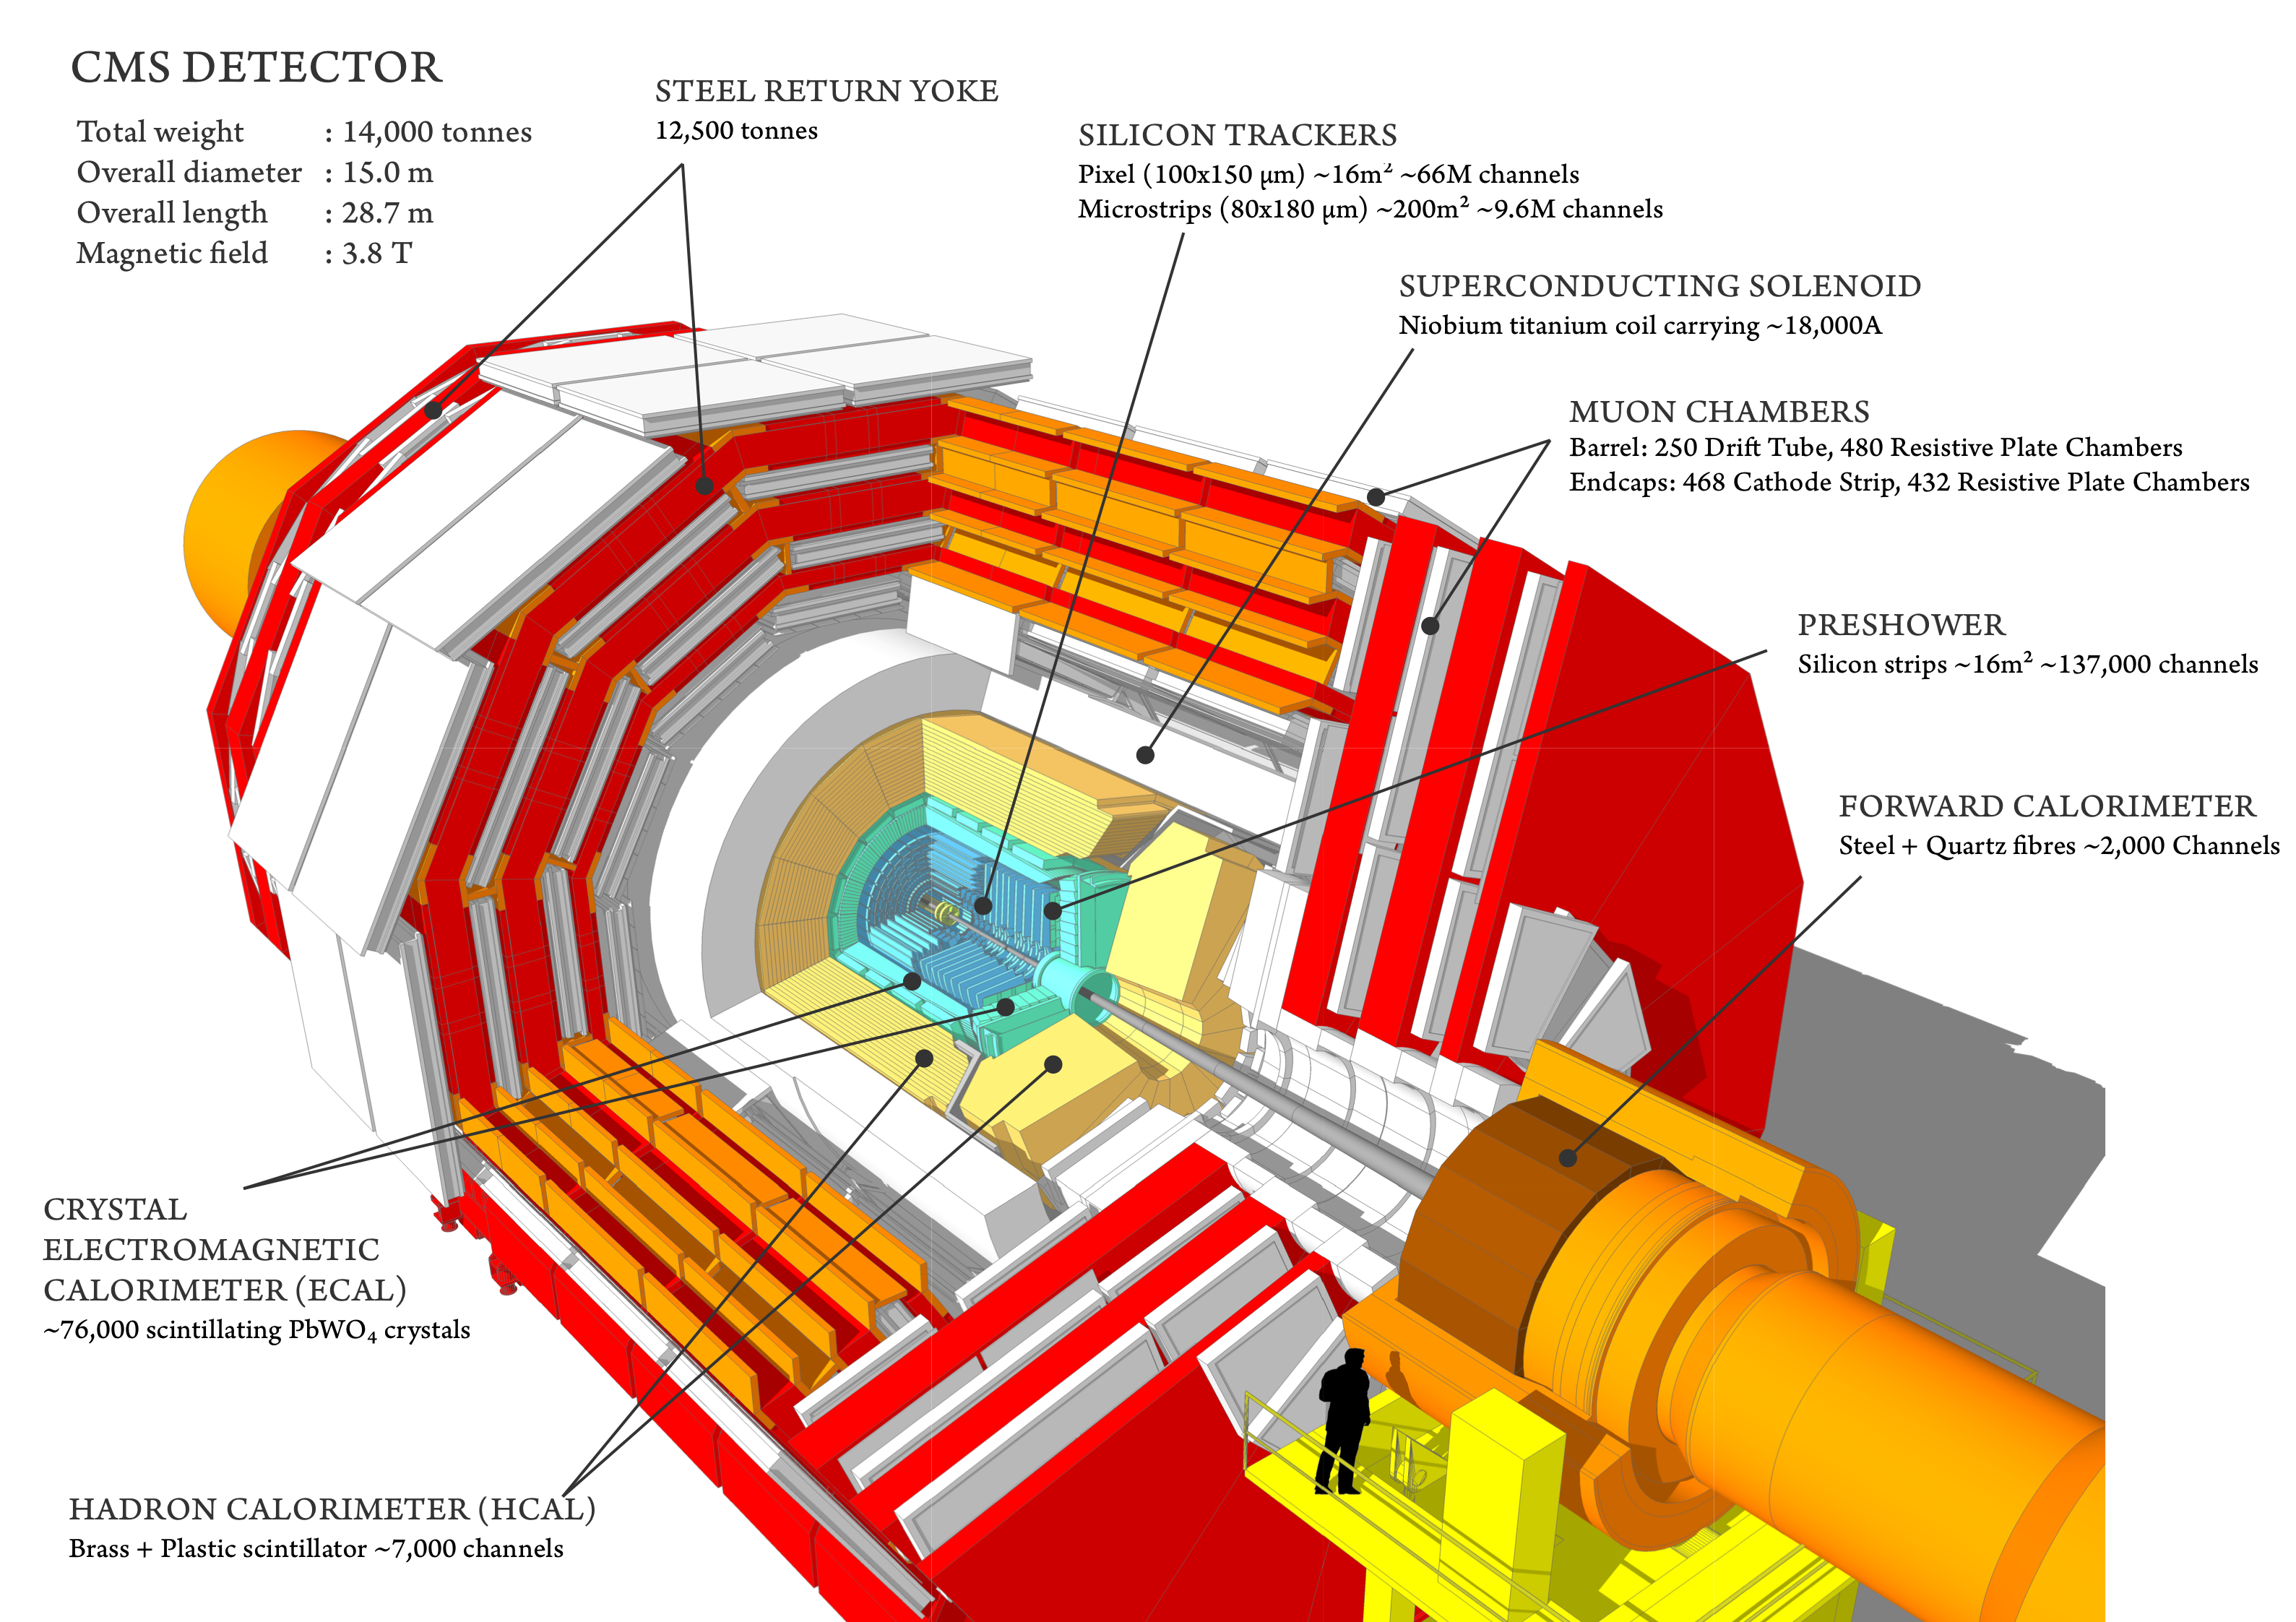
\includegraphics[width=\textwidth]{figures/LHCandCMS/CMScutaway.png}
  \caption{
    A cutaway view of the CMS detector, showing each detector 
    subsystem~\cite{1742-6596-513-2-022032}.
        }
 \label{fig:CMScutaway}
\end{figure}

The coordinate system adopted by CMS, and used in this thesis,
is a right-handed coordinate system with the point $(x, y, z) = (0, 0, 0)$
centered in the detector, at the nominal collision point. The $y$-axis 
is perpendicular to the earth, where vertically upward defines the $+y$ direction.
The $x$-axis is in the plane of the LHC, with the $+x$ direction pointing towards
the center of the ring. The $z$-axis points through the center of the detector
along the direction of travel of the colliding protons, where $+z$ is defined
by the right-handedness of the coordinate system. In polar coordinates, 
the azimuthal angle $\phi$ is measured from the $x$-axis in the $x$-$y$
plane, and the polar angle $\theta$ is measured from the $z$-axis. The radial
coordinate $r$ is defined as $r = \sqrt{x^2 + y^2 + z^2}$.
Because the production of 
particles is preferentially in the forward direction (along
the $z$-axis), it is convenient to introduce the pseduorapidity $\eta = - \ln(\tan{\theta/2})$
for the polar coordinate. The momentum in the transverse direction,
defined as $\pt = \sqrt{p_{x}^2 + p_{y}^2}$, is a particularly important quantity.
because the initial transverse momentum of the collision is zero.
In this thesis, the four-momentum of an object will commonly be expressed as
$p = p(m, \vec{p}) = p(m, \pt, \eta, \phi)$.

\section{The CMS solenoidal magnet}

The central feature of the CMS apparatus is a superconducting solenoid 
of $6\unit{m}$ internal diameter and $12.5\unit{m}$ in length,
constructed from 4 layers of reinforced niobium titanium.
It provides a nearly constant $3.8\unit{T}$ magnetic field inside the solenoidal volume.
The magnetic flux of the solenoid is returned through
a $12 000$-tonne steel yoke, comprising 5 wheels and 2 endcaps,
which is fully saturated to approximately $2\unit{T}$. 
The tracker and calorimeters are situated inside the solenoid, while 
the muon detectors are embedded in the steel return yoke, as shown
in Fig.~\ref{fig:CMScutaway}.

During operation, the CMS solenoid stores approximately $2.4\unit{GJ}$ of 
energy, the largest magnet in the world by this metric. This immense
size leads to a powerful bending radius for charged objects within the detector,
which is a critical metric for particle reconstruction and identification.
In particular, objects of charge $q$ moving
in a magnetic field $\vec{B}$ at velocity $\vec{v}$ experience a Lorentz force,

\begin{equation}
  \vec{F} = q\vec{B} \times \vec{v} \,.
\end{equation}

Because the solenoidal field is constant and aligned along the $z$-direction, 
$\vec{B} = B\hat{z}$, the force is purely in the transverse direction.
Consequently, charged particles within the CMS
solenoid travel along a nearly helical path of radius $R=\pt/\abs{q}B$, where 
small deviations from this path arise from non-uniformity of the field
and interactions in the detector material. The sign of a 
$\pt$ of a particle of known charge can therefore be deduced by measuring its radius of
curvature. The bending power of the magnet $BR$ is therefore a critical 
parameter determining the detector capability for accurate particle $\pt$ measurement.
The nearly $12\unit{Tm}$ bending power achieved by the CMS is critical to achieving
the high momentum resolution outlined in the design goals of the experiment. It
is also fundamental to the particle flow reconstruction technique utilized by CMS,
outlined in Chapter~\ref{ch:reconstruction}.

\section{The CMS silicon tracking system}

Stuff about this

\section{The CMS electromagnetic calorimeter}
\section{The CMS hadronic calorimeter}
\section{The CMS muon system}

As suggested by the CMS name itself, the muon detector subsystem is essential to the
achieving the experimental goals of the CMS experiment. 
High-energy muons are produced in many heavy-object SM and BSM 
decays, and long-established detector technologies are well suited to muon detection in LHC collisions.
Muons with $v\approx c$ are nearly stable
on timescale of the traversal of the CMS detector volume. As the heavies stable lepton, 
they are less susceptible to electromagnetic radiative energy loss than electrons, and therefore
interact minimally with the calorimeter system. Detector technologies suitable for
charged-particle detection, placed outside all other detector systems, 
are therefore ideal for muon detection. 

\begin{figure}[htbp]
  \centering
   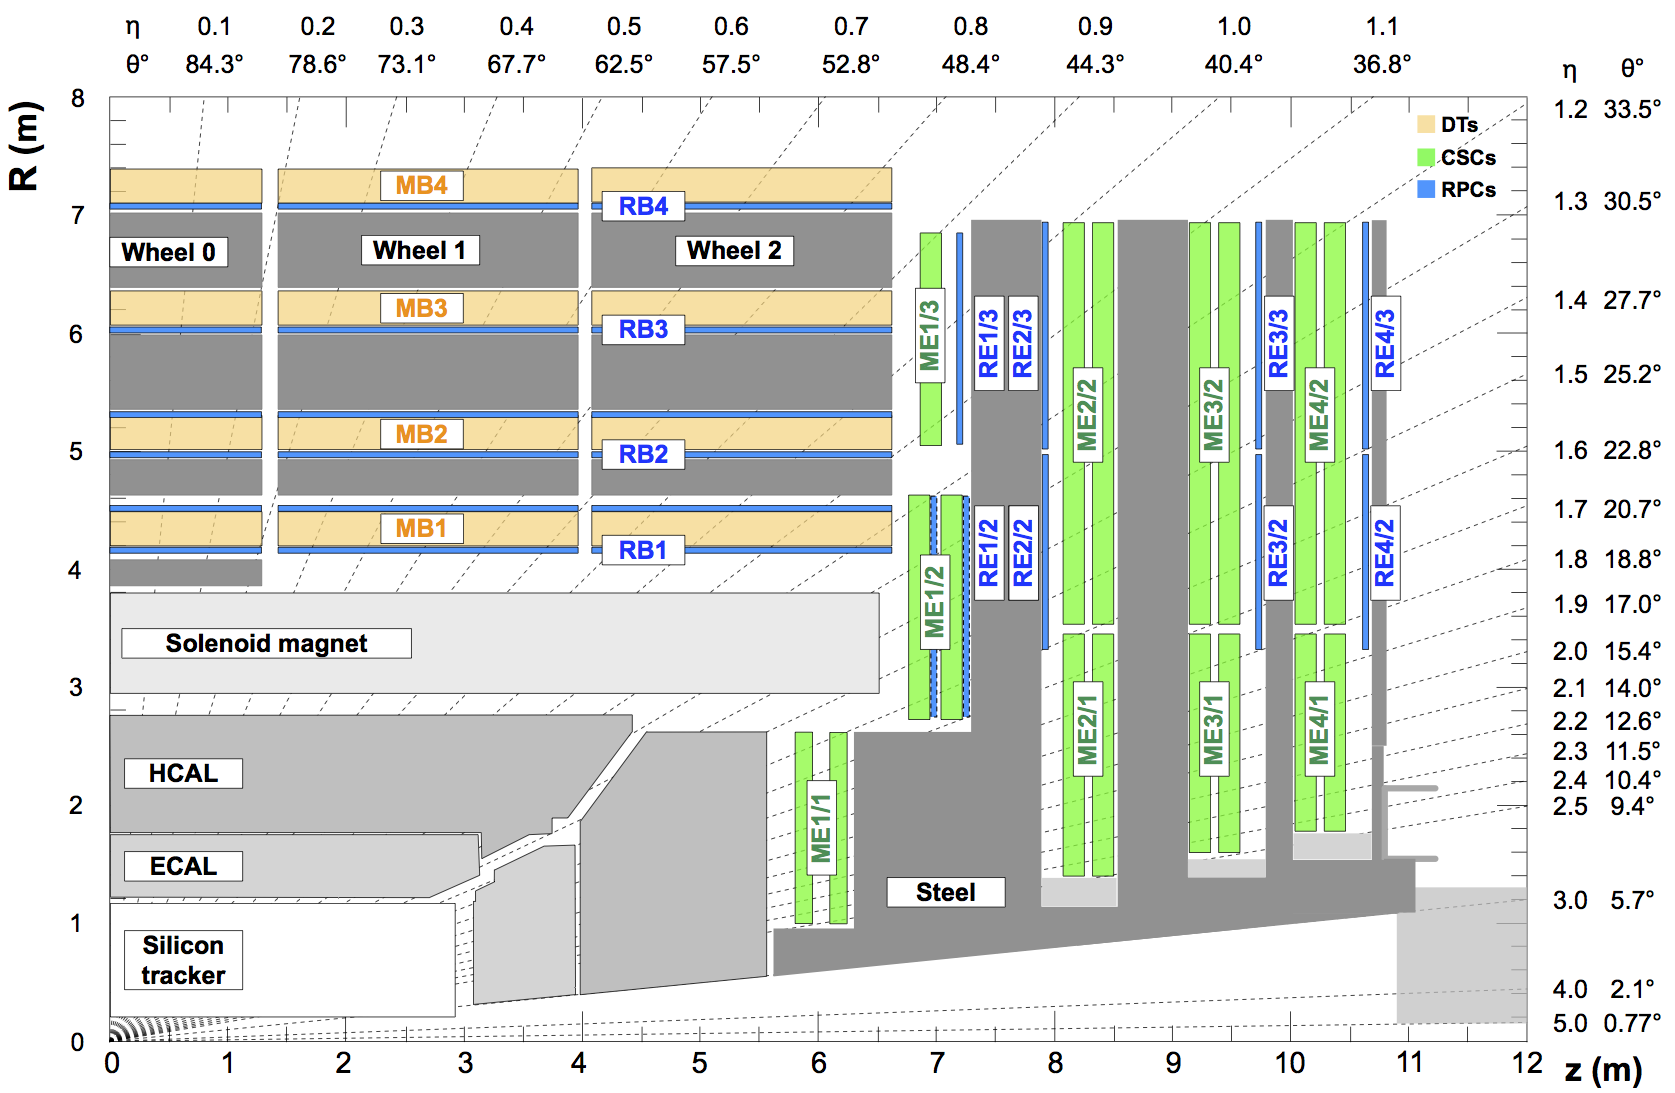
\includegraphics[width=\textwidth]{figures/LHCandCMS/MuonSystemGeometry.png}
  \caption{
    An $R-z$ cross section of a quadrant of the CMS detector, with the interaction
    point at the bottom left corner. The locations of the detectors
    comprising the CMS muon system within the steel steel return yoke
    are shown~\cite{Chatrchyan:2012xdj}.
        }
 \label{fig:muonSystemGeo}
\end{figure}

The muon system is composed of three technologies, 
described in more detail in the following sections. 
Each operates on the principle of gas ionization. 
The detectors consist of a volume of 
gas over which an electric field is applied. Charged
particles passing through the volume ionize the gas, and the ionized gas molecules
and free electrons drift in the electric field towards read-out electronics at the 
edges of the detector volume. The track of the interacting object is inferred from
the position and timing of the measured electrons and ions.
The operating characteristics of the gas ionization detectors can be modified
for fast readout, high granularity, and 
In the CMS detector, these considerations, along with the cost of construction 
for detectors covering an area of $\\approx 25,000\unit{m}^2$ and 
the effect of the radiation environment of the detector on performance, motivate
the specific design choices.

Gas ionization detectors are
sensitive to all charged particles passing through the detector. As previously discussed,
nd illustrated in Fig.~\ref{fig:muonSystemGeo}, the muon system is 
the outer layer of the CMS detector, embedded in
the steel return yoke of the magnet system. This structure, along with the inner
detector systems, serves as shielding for the muon system and ensures that the 
well over 99\% of objects reaching the muon system are muons.

\subsection{Drift tube system}

The barrel part of the muon detector, $\abs{\eta} < 1.2$,
is composed of drift tube (DT) chambers. In this region, the magnetic field
outside the return yoke is generally small (below 0.2\unit{T}), and the muon occupancy is low, justifying
the use of DT detectors. The DT system is built from individual DTs, 
rectangular aluminum tubes with a length of 2.4\unit{m} and a cross section
of $13\times42\unit{mm}^2$, shown in Fig~\ref{fig:DTs}. At the center of each
tube is a 50-\micron-diameter gold-plated stainless-steel anode wire.
Aluminum strips are attached to the interior of the aluminum 
structure---insulated by mylar tape---to
shape the electric field to the pattern illustrated in Fig.~\ref{fig:DTs},
and an 85\% Ar 15\% CO$_2$ gas mixture is contained in the volume. 
The drift time for muons crossing a
cell at a maximum distance from the anode wire of 21\unit{mm}
is about 380\micron, which is sufficient to keep the occupancy low.
Muons passing through the gas volume ionize the gas and create an avalanche of
electrons around the very high field at the anode wire.
A time-to-digital converter reads out the electrical pulse of the electrons.
The arrival time of the signal, corrected by the drift velocity and the time
from the collisions to the trigger decision, are used to obtain the muon interaction
position. 

\begin{figure}[htbp]
  \centering
   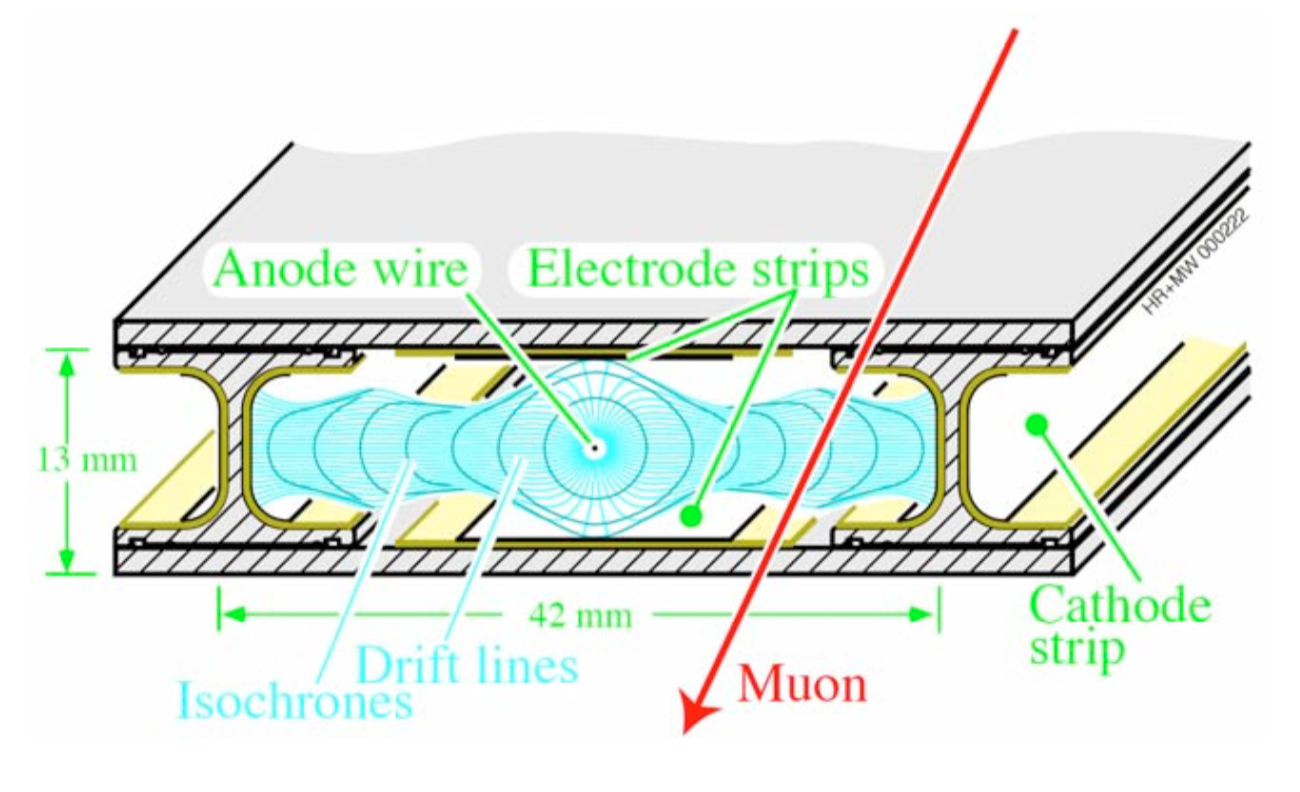
\includegraphics[width=0.6\textwidth]{figures/LHCandCMS/DriftTubeCutaway.png}
  \caption{
    Diagram of a drift tube cell, from Ref.~\cite{Chatrchyan:2008aa}. The 
    geometry of the cell and the electric field lines resulting from the 
    anode wire and electrode strips are illustrated.
        }
 \label{fig:DTs}
\end{figure}


The DT cells are assembled into superlayers (SL), composed of 
4 layers of drift cells staggered by half a cell. 
The SLs are grouped into chambers of 2 or 3 SLs which are arranged into stations
within the magnet return yoke.
The wires in the outer SLs within a chamber are parallel to beam line, providing
a measurement in the bending plane.
An additional inner SL is aligned perpendicular to the beam direction, 
for all chambers but those in the 
outermost station, to provide a measurement in the $z$ plane. 
The chambers are arranged in concentric cylinders
around the beam line, with 60 chambers each in the three inner cylinders
and 70 in the outer cylinder. In total there are $\approx172,000$ 
cells, read out as independent channels. The offset arrangement of the cells
eliminates dead spots in the efficiency, and allows a measurement of the
muon crossing time to be obtained using meantimer circuits.
The muon position resolution in the DTs is around 100\micron and the
timing resolution is within a few ns.

\subsection{Cathode strip chamber system}

Cathode strip chambers (CSC) are used in
the forward regions of the CMS detector ($0.9 < \abs{eta} 2.4$), 
where the prompt and background muon rates are high, and the magnetic field
is large and non-uniform. The CSC system is constructed of trapezoidal
multi-wire proportional chambers,
which subtend 20 or 30 degrees in $\phi$. The largest chambers are 3.4\unit{m}
long and up to 1.5\unit{m} wide. The chambers are divided into 6 sections---7\unit{mm} 
wide for the innermost layer of chambers and 9.5\unit{mm} for all 
others---each filled with an Ar-CO$_2$-CF$_4$ gas mixture. Aluminum cathode strips,
which span the radial direction at a constant phi, 
are milled to 6 of the panels forming the sections. The strips vary from
8.4 to 16\unit{mm}, for a constant width in $\phi$, and are separated by about 0.5\mm. 
In addition, each layer has a planes of anode wires running lengthwise, 
50\micron in diameter, separated by 2.5\unit{mm}, and slightly tilted to correct
for the deflection of the drifting electrons in magnetic field.
Muons passing through the chambers create and avalanche
of electrons in each layer, which is read out on the anode wires. In addition,
A mirror pulse is created in the cathode strips.
Together, the pulses and shapes give an excellent position measurement 
in both the $r-\phi$ and $\eta$ planes, as shown in Fig~\ref{fig:CSC}.
Each cathode strip is read out, whereas anode strips are read out in
groups of 16. The position resolution of a CSC chamber is around
100\micron, and the timing resolution is $\approx7\unit{ns}$

\begin{figure}[htbp]
  \centering
   \includegraphics[width=0.49\textwidth]{figures/LHCandCMS/CSCdiagram.png}
   \raisebox{0.3\height}{\includegraphics[width=0.49\textwidth]{figures/LHCandCMS/CSCoperation.png}}
  \caption{
    Left: diagram of a CSC chamber. Right: principle of operation for a CSC
    layer, showing the avalanche around the anode wires and the pulse shape
    on the cathode strips, which are combined for accurate position measurement.
    Both figures are reproduced from Ref.~\cite{Chatrchyan:2008aa}
        }
 \label{fig:CSC}
\end{figure}

The CSC chambers are arranged perpendicular to the beam line,
conjoined for full coverage in $\phi$. Four stations of CSC chambers are interspersed
amongst the magnetic flux return plates in each endcap of the detector, see
Fig~\ref{fig:CMScutaway}. The innermost station (for each endcap) is composed of 
3 rings of CSC in the radial direction, whereas other stations have two rings.
In total there are 540 CSC chambers. All but the outer ring of chambers in the 
innermost layer partially overlap the neighboring chambers, avoiding regions
of low efficiency. Aging studies of the CSC chambers at the original CERN Gamma
Irradiation Facility (GIF), and at the new GIF++, have shown that the CSC system
performance is resistant to the damage incurred by the radioactive environment
of high luminosity collisions. 

\subsection{Resistive plate chamber system}

A crucial role of the muon system is to provide muon position and momentum
measurements in a sufficiently timescale
to determine if an event justifies storage offline analysis. 
This process, known as event triggering,
is described in additional detail in Section~\ref{sec:triggering}.
While the DT and CSC system provide fast readout, the background rate and
importance of associating an event with the correct bunch crossing (within
25\unit{ns}) make additional redundancy desirable.

A system of resistive plate chambers (RPC) in both the barrel and endcap
($\abs{\eta} < 1.2$ accomplishes this goal. The RPCs are double-gap chambers
constructed from a thin layer of readout strips between two electrodes held 
at high voltage, forming a volume filled predominately with C$_2$H$_2$F$_4$ gas.
The system is operated in avalanche mode, where the sum of the signals
in the two gaps created by an interacting muon is read out on strips
at the center plate. The plates are separated by 2\unit{mm}, which ensures
that the charge avalanche is observed well below the 25\unit{ns} window
needed to assign the muon to the correct bunch crossing.
There are 6 layers of RPCs in the detector barrel, interspersed among the DTs,
and 3 layers in the endcap alongside the CSCs. The readout strips in the barrel RPCs
subtend an angle of 5/16 degree. The position resolution of the RPCs, about 1\cm,
is below the DT and CSC systems, but the system provides an independent position
and timing measurement. 

\section{Data triggering and acquisition}
\label{sec:triggering}
\section{Luminosity measurement}

\chapter{Theoretical predictions and event simulation}
\label{ch:simulation}

Quantifying the agreement of experimental observations with the SM
or with possible BSM theories is a core goal of collider physics.
While the SM is a nearly complete and profoundly successful theory,
connecting theories which concern the interactions and excitations of quantum fields
to the electrical signals induced in the CMS detector by
\pp collisions is highly non-trivial.
In an ideal case, one would use
the theory of particles and fields outlined in Chapters~\ref{ch:introduction} 
and \ref{ch:phenomenology} as input to derive the expected distribution
of measurable signals resulting from \pp collisions.
In this paradigm, BSM modifications to the SM are realized as modifications 
to the structure of the underlying QFT. They lead to new interactions, which
modify the rate or type of particle production, or kinematics variables 
of the produced particles, leading to deviations from the SM expectation
in measured quantities. 
In practice, a factorized approach---leveraging approximations and tuning 
to experimental data---allows the simulation of primary particle production in
\pp collisions, the formation of bound states and particle decay,
and the interactions of particles in the CMS detector 
to be simulated in a way that largely achieves this goal.
The CMS Collaboration benefits from the work of collaborations of theoretical 
physicists and many previous studies to achieve detailed simulations.

It is important to highlight that the experimental physicists
is not purely at the mercy of the simulations from which our predictions derive.
Many predictions are phenomenological in nature, i.e., they have been tuned to the 
observations measured in LHC collisions and previous accelerators.
Furthermore, in situ measurements allow the data observation 
to modify aspects of the predictions. Lastly, broad knowledge of the nature
of particle production in collisions can sometimes be leveraged to completely 
remove dependence on simulation. For example, with no resonant source of 
diphoton production, the $m_{\gamma\gamma}$ distribution would be a falling spectrum.
The first measurements of the scalar Higgs boson with $m_{\PH} = 125\GeV$ made 
in the diphoton channel where achieved with the SM $\pp\to\gamma\gamma$ 
expectation parameterized as a falling exponential distribution,
not with an ab initio simulation of the distribution~\cite{Aad:2014eha,Khachatryan:2014ira}.

Nonetheless, the results presented in this thesis concern the measurement
of a rare SM process. In particular, determining the production mechanism
of {\WZjj} production and identifying the component that is sensitive to the
\WWZZ coupling relies heavily on achieving well-understood simulations of the
signal and background processes contributing to the events analyzed.
This chapter discusses the techniques used to simulate \pp collisions at the
LHC. The techniques used to obtain results for \WZjj production in the SM and beyond,
and the prediction used in this analysis, are presented. 
Their impact on the analysis and the role of the analysis in assessing the predictions
is discussed.

\section{Anatomy of an LHC collision}

As discussed in Chapter~\ref{ch:penomenology}, perturbation theory is the 
most effective technique for calculations of particle scattering in
the SM QFT. While the underlying principles are well-established, calculations
of QCD interactions, in particular, are computationally challenging. The QCD 
theory is asymptotically free, meaning $\alpha_s(\mu)$ grows with low values of 
the energy scale $\mu$, so low-energy phenomena are non-perturbative.
Because asymptotic freedom also leads to bound states at the low 
energy scales of most physical phenomena, the energy regime of stable particles---and
therefore the incoming state directed to collision and the outgoing particles
that interact with the detector---have non-perturbative properties.

The uncomfortable dichotomy between the regime of most physical phenomena and calculability
is averted by the concept of factorization, which allows a separation of short-distance
interactions from long-distance interactions, or equivalently, interactions governed
by energy scales large or small with respect to $\lqcd\approx 200\MeV$.
Factorization states that the interaction
of hadrons can be reduced to structure functions describing the distribution of quarks
and gluons in hadrons, known as parton distribution functions (PDF), convoluted
with the parton-parton interaction cross section. At high momentum transfer,
the parton-parton interaction can be described perturbatively. Furthermore,
the evolution of the interaction from outgoing quarks, gluons, and leptons
can be factorized from the formation of bound states, described by 
parton-to-hadron fragmentation functions, and their decay. The concept is illustrated
for \pp collisions in Fig.~\ref{fig:factorization}.
Factorization 
is formally established under certain conditions~\cite{Collins:1989gx}, and it 
has been highly successful in describing experimental observations over generations
of hadron-hadron, lepton-lepton, and hadron-lepton colliders.

\begin{figure}[htbp]
  \centering
   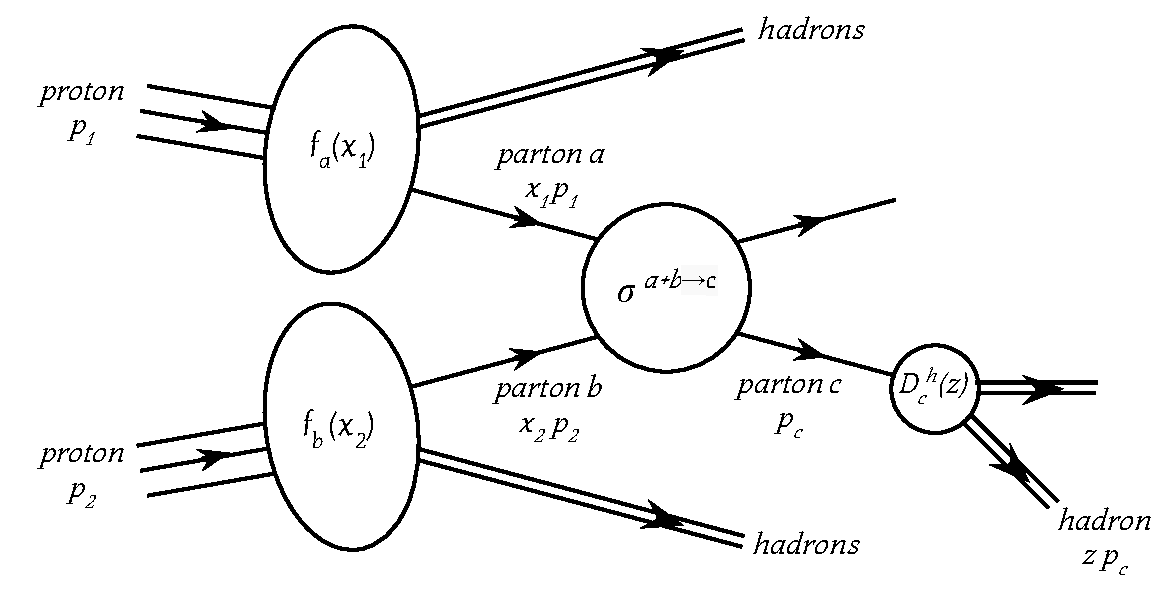
\includegraphics[width=0.6\textwidth]{figures/Simulation/factorization.pdf}
  \caption{
    Illustration of the principle of QCD factorization. The cross section
    of the process $\pp\to X$ is reduced to the parton distribution
    functions $f_{a,b}(x)$, the partonic cross sections $\sigma^{a+b\to c}$,
    and the parton-to-hadron fragmentation functions $D_{c}^{h}(z)$.
    Reproduced from Ref.~\cite{Adare:2014hsq}.
        }
 \label{fig:factorization}
\end{figure}


Factorization allows the challenge of describing LHC collisions to be
tackled in pieces, leveraging different techniques for each piece while benefiting
from possibly independent experimental data. 
This chapter summarizes how these factorized components are modeled
for the simulations that are used to guide in this analysis.
In some cases, it is useful to consider only some contributions.
For example, the effect of the experimental
reconstruction can be parameterized by reconstruction efficiencies, or the hadronization
of quarks and gluons can be reduced to an effective smearing, 
in cases where the effects are not dramatic and are well-established. 
Such predictions are also presented, and their relevance to this
analysis is discussed.

\section{Parton distribution functions}

One of the fundamental ideas of factorization is that the low-energy confinement
of quarks and gluons in the proton can be described independently from the 
parton-parton interaction in a hard collision, e.g., momentum transfer 
$Q^2 \gg \lqcd^2$. Mathematically, the 
separation of the proton structure and the high-$Q^2$ parton interaction,
shown pictorially in Fig.~\ref{fig:factorization}, can
be expressed as
\begin{equation}
  \sigma^{\pp\to X} = \sum_{a,b\in\{q,g\}}\int{\mathrm{d}x_1\mathrm{d}x_2f_{a}(x_1, \muF^{2})f_{a}(x_2,\muF^{2})}
      \hat{\sigma}^{\Pq\Pq'\to X}(x_1x_2s, \muF^{2})
\end{equation}
where $x_1$ and $x_2$ are the momentum fractions of the proton momentum carried by 
partons $a,b \in \{q,g\}$ and the PDFs $f_{a,b}(x_i)$ give
the probability of extracting the given parton with momentum fraction $x_{i}$.
The total momentum must be divided amongst the constituents, i.e.,
\begin{equation}
  \sum_{i}\int_{0}^{1}\mathrm{d}x xf_{i}(x, \muF^2) = 1
\end{equation}
Here $\muF$ is the factorization scale, an energy scale which represents the transition
from the non-perturbative regime of the PDF and the perturbative high $Q^2$ interaction.
Thought it is often convenient to take $\muF=Q^2$, $\muF$ is a free parameter that is an
artifact of the truncated serious in perturbation theory. As the order of the perturbation
expansion considered increases, the $\muF$ dependence of the result is reduced.

At least to very good approximation, the PDFs can be considered universal functions. 
Therefore, they can be derived using independent measurements, such as
deep inelastic scattering of lepton and proton beams. As shown in Fig.~\ref{fig:dis}, a lepton
incident on a proton target interacts with the quarks of the proton via a virtual
$\gamma$ or {\cPZ}. By controlling the incident energy of the proton and lepton and
measuring the outgoing particles the abundance and momentum fraction of the proton
constituents can be established.
\begin{figure}[htbp]
  \centering
   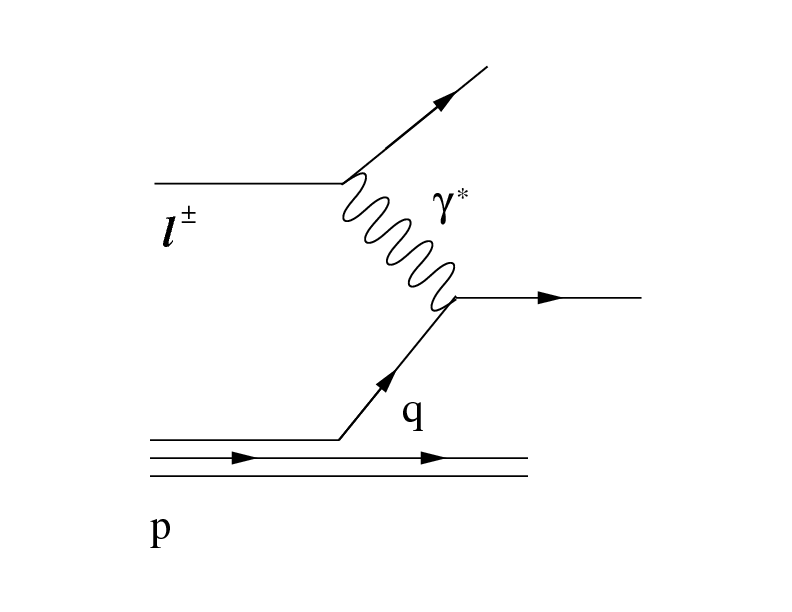
\includegraphics[width=0.4\textwidth]{figures/Simulation/DIS.png}
  \caption{
    Illustration of deep inelastic scattering of a lepton from a proton, used
    as a probe of the internal parton structure of the proton.
    Reproduced from Ref.~\cite{Filippone:2001ux}.
        }
 \label{fig:dis}
\end{figure}

In practice, it is not feasible to parameterize all partons (and flavors) for
all $x_{i}$ through experimental measurements. Fortunately, while perturbation theory
cannot predict the formation of bound states, it does allow a means to 
parameterize the evolution of the bound partons across energy scales. The scale
dependence of the PDF is captured by the DGLAP equations, first established
by Dokshitzer~\cite{Dokshitzer:1977sg}, Gribov~\cite{Gribov:1972ri}, 
Alterelli and Parisi~\cite{Altarelli:1977zs} in the 1970s:
\begin{equation}
  \muF^2\frac{\mathrm{d}f_{a}(x, \muF^2)}{\mathrm{d}muF^2} =
    \sum_{b\in\{q,g\}}\int_{x}^{1}\frac{\mathrm{d}z}{z}\frac{\alpha_s}{2\pi}
    \hat{P}_{ba}(z))f_b(x/z,\muF^2 \,.
\end{equation}
The functions $\hat{P}_{ba}(z)$ are the Alterelli--Parisi splitting functions,
which describe the splitting of parton $a$ into $b$, carrying a momentum
fraction $z$ of the initial momentum, that
can be derived order by order in perturbation theory. The splitting of
parton $a$ is accompanied by an additional parton, e.g., $\Pg\to\Pq\Paq$,
that is absorbed in to the parton sea of the proton. Given the DGLAP equations,
if the proton PDF can be established for any complete phase space of
parton flavors, momentum fractions, and $Q^2$, it can be evolved to all other 
scales. In practice, the contributions to the PDF are
at many different $Q^2$ with experiments sensitive to different quark flavors.
The experimental data is fitted, considering the DGLAP evolution, to obtain
a full parametrization of the PDF at all energy scales. 

Collaborations of theorist use independent techniques to fit data
from many collider and fixed target experiments to produce large data sets
of predictions that can be used in simulations. The PDF is parameterized
and distributed as data grids that can be sampled with a centralized interfaced
known as LHAPDF~\cite{Buckley:2014ana}. Results in this thesis primarily
make use of the NNPDF3.0~\cite{NNPDF2015} set of PDFs, which use a neutral net and generated
pseduodata to perform global fits to the data. 
Uncertainties in this procedure and their impact on this analysis 
are discussedin Chapter~\ref{ch:analysis}.
They are assessed by evaluating the quality of the PDF fit to the data, 
comparing the predictions of independent collaborations
in a formulaic way~\cite{Butterworth:2015oua}, and by determining
the dependence of predictions on $\muF$.

\section{Perturbative calculations and matrix element generators}

With the parton content of the proton captured by the PDFs, the next challenge
in modeling an LHC collision is the perturbative calculation of the parton-parton
interaction. As discussed in Chapter~\ref{ch:phenomenology}, perturbation theory
relies on an expansion in the coupling constants of the theory,
\begin{equation}
  \sigma = \sigma_0\alpha_s^{0} + \sigma_1\alpha_s^{1} + \sigma_2\alpha_s^{2} + \cdots\,.
  \label{eq:pqcd}
\end{equation}
For a process with only by EW couplings at the lowest order, such as VV production,
$\sigma_0 = \sigma_{LO}$ and $\sigma_1 = \sigma_{NLO}$.
While $\alpha_s$ is sufficiently small at the LHC collision energy to justify the
perturbative expansion ($\alpha_s(m_{\PZ}) = 0.1189 \pm 0.0010$~\cite{Tanabashi:2018oca}),
the energy and phase-space dependence of higher-order terms is non-trivial,
leading to QCD corrections much larger than the naive 
expectation in many cases~\cite{Altarelli:1979ub,Campbell:2011bn,Dittmaier:2011ti}.
The majority of production processes at the LHC require a calculation at least to NLO in QCD for percent-level accuracy.
Theoretical tools have advanced to allow automated computation of all 
SM processes at NLO~\cite{Gleisberg:2008ta,MGatNLO,Recola},
and many processes have recently been computed at NNLO in QCD~\cite{Grazzini:2017mhc}.
Calculations
at LO in the EW theory are often sufficient for percent-level accuracy. However,
some processes are susceptible to anomalously large EW corrections, including
VBS VV production~\cite{Biedermann:2016yds}, considered in this thesis.

The cross section of Equation~\ref{eq:pqcd} can be expressed in terms of the square of 
the scattering matrix element $\mathcal{M}$, which 
captures the transition probability from the initial to the final state.
The matrix element, or scattering amplitude, is calculable in perturbation theory, of which
techniques based on Feynman diagrams are the most familiar. 
Because the total cross section is a scan over all possible outgoing energy and momenta
combinations of the outgoing particles, the cross section is an integration over a
many-dimensional phase space of configurations $\Phi_{n}$,
\begin{equation}
  \sigma_{i} = \int \mathrm{d}\Phi_{n}\left|\mathcal{M}_i\right|^2 \,.
  \label{eq:meint}
\end{equation}
The integration can be performed with numerical techniques. The high dimensionality
of the phase space, as well as the complex peak structure arising from resonances,
is well-suited for Monte Carlo integration techniques, described in the following section.

In the Feynman diagram approach to matrix-element calculations, amplitudes are represented by Feynman diagrams
where QCD (EW) coupling vertices in the diagrams are proportional to $\sqrt{alpha_s}$ ($\alpha$).
A calculation at a given perturbative order involves all diagrams connecting 
desired initial and final states for which the product of vertices is less than the order
of the perturbative expansion.
Feynman diagrams can be generated in an automated procedure with techniques from graph theory, 
before being used to derive and calculate amplitudes from Feynamn rules in the SM.
Automation of this process was established in the early 1990s at LO~\cite{Stelzer:1994ta}.
Extending this to procedure to NLO has been accomplished more recently by the 
program \MG~\cite{MGatNLO}, the successor to the previous work, which is the used extensively
for results in this thesis.

Diagrams without loop contributions are called ``tree-level'' diagrams. The lowest tree-level
contribution to a given state, shown for $\pp\to\PW\PZ$ in Fig.~\ref{fig:WZNLO} (far left),
is referred to as the Born-level contribution to the process. The NLO correction to the Born
process includes contributions from tree-level diagrams of $\pp\to\PW\PZ+\jet$ for $\jet\in\{\Pg,\Pq\}$, 
known as real emission diagrams, and loop contributions, shown in Fig.~\ref{fig:WZNLO} (center)
and (left) respectively. 
Divergences from each of these contributions cancel through
renormalization. The delicate procedure of ``cancelling infinities'' via numerical techniques,
presents a major challenge to automating NLO calculations.
It requires a cut to be made precisely at the infinite pole, and 
careful management of the divergent contributions around the pole with high-precision numerical accuracy.
All possible one-loop amplitudes in the SM have been calculated with analytic techniques.
Automated codes access these loop contributions and residual divergences from packages such as
OpenLoops~\cite{Cascioli:2011va}, and combine them with the Born and real-emission calculations,
while verifying that the infinities of the loop and real-emission calculations do indeed cancel.
As the first NLO calculations became available, the interplay between contributions was
adjusted per process in dedicated calculations. For example in Refs. for the \WZ process
and Refs. for \EWWZ.
This procedure is now automated in several general-purpose MC programs
used in this analysis, including
\MG~\cite{MGatNLO}, \Sherpa~\cite{Gleisberg:2008ta}, \Herwig~\cite{Bellm:2015jjp}, and \Recola~\cite{Recola}.
However, programs which automate all SM calculations are not optimized for specific
process, which can lead to prohibitively long computation time for high-multiplicity states
or processes with a complex phase, such as \EWWZ. For this reason, the best-available
calculations for the \QCDWZ and \EWWZ process come from dedicated implementations, such as
Refs.~\cite{Bozzi:2007ur,Campanario:2013qba}.

\begin{figure}[htbp]
  \centering
   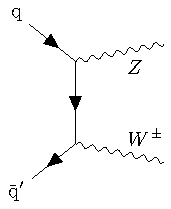
\includegraphics[page=1,width=0.22\textwidth]{figures/FeynmanDiagrams/WZNLOfeynman.pdf}
   \includegraphics[page=2,width=0.22\textwidth]{figures/FeynmanDiagrams/WZNLOfeynman.pdf}
   \includegraphics[page=3,width=0.22\textwidth]{figures/FeynmanDiagrams/WZNLOfeynman.pdf}
  \caption[Contributions to the $\pp\to\WZ$ process at NLO]{
    Contributions to the $\pp\to\WZ$ process at NLO. The leftmost diagram is the Born
    contribution, which is part of the LO calculation. The real-emission diagram
    is shown in the center, and the loop contribution is far right. The cross section
    is proportional to the square of the sum of amplitudes shown, which at 
    $\mathcal{O}(\alpha_s)$ includes the square of the Born and real-emission diagrams
    and the interference of the loop and Born diagrams.
  }
 \label{fig:WZNLO}
\end{figure}

Diboson processes inclusive in the number of jets have recently become available 
at next-to-next-to-leading order (NNLO)~\cite{Grazzini:2017mhc}. These calculations
have an additional layer of complication due to the more complex cancelling of
divergences between double loop, double real-emission, and combined real-emission
and loop contributions. They are not yet automated,
partially because not all two-loop amplitudes in the SM are known.
Combining these predictions with hadronization functions,
discussed in the following sections, is also not yet accomplished for diboson
processes. In this thesis, we use NNLO cross section calculations to 
correct the predicted yields of NLO simulations for diboson processes.

\section{Monte Carlo integration and event unweighting}

As referenced in the previous section, calculations of physical
quantities involve integrations of the amplitude over the relevant phase space
for the scattering process. Because the solution


The phase space integration in Equation~\ref{eq:meint}
is an integration over the quantum numbers and four-momenta of all particles 
considered. The integration is often complex and rarely solvable analytically.
Solutions can be obtained numerically, leveraging techniques which have
been widely studied in applied mathematics and computer science~\ref{}.
Because of the high-dimensionality of the integration, an algorithm 
for which the uncertainty scales independently of the dimensionality is highly 
desirable. For this reason, a technique based on random numbers known as 
Monte Carlo (MC) integration is used~\cite{doi:10.1002/wics.1314}. The algorithm
was first formally developed in the late 1940s as part of the Manhattan project,
with the name derived from the eponymous casino for due to its leveraging
of random processes~\cite{10.2307/2280232}.

The MC procedure estimates 
the integral of a function $f(x_{i},\cdots,x_n\equiv\vec{x})$, defined over a volume $V^{n}$,
is estimated by tossing random random points inside a known volume
over which the function is defined, of dimension $V^{n+1}$. The volume $V^{n+1}$
from which the random numbers are drawn must fully contain 
$f(\vec{x})$, however, no further knowledge of $f(\vec{x})$ over $V^{n+1}$ is required. The function
is evaluated for the coordinates $x_i\cdots x_n$ of the random point.
If the random point is inside the volume of $f(\vec{x})$, it is accepted,
if it falls in a region of $V^{n+1}$ outside of $f(\vec{x})$ it is rejected.
As the number of points sampled $N$ grows, the ratio of the number of accepted
points to $N$ times the volume of $V^{n+1}$ approaches the integral of $f(\vec{x})$.
This is illustrated for one dimension in Fig.~\ref{fig:mcintegration}.
The error of the integration decreases proportional to $\sqrt{N}$, which
is very poor for low dimension integration ($\lesssim$4) but much better than
traditional techniques for high-dimensional problems.

\begin{figure}[htbp]
  \centering
   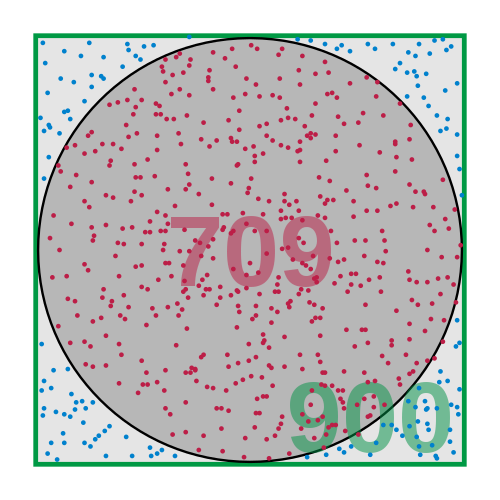
\includegraphics[width=0.6\textwidth]{figures/Simulation/MCintegration.png}
  \caption[Illustration of the principle of Monte Carlo integration.]{
    Illustration of the principle of Monte Carlo integration. If the area
    of the rectangular phase space is known, the area of the circle can
    be estimated from the ratio of randomly sampled points falling
    inside or outside the volume. In this example, the ratio of accepted
    points (709, red) to the total points sampled (900) approximates the
    analytic result for the ratio of the areas, $\pi/4$.
    Reproduced under public license from Ref.~\cite{wiki:mc}.
        }
 \label{fig:mcintegration}
\end{figure}

In addition to predictions for aggregated quantities such as total cross sections
and differential rates, event-wise simulations are critical to modeling expected 
results in the realistic environment of particle physics measurements.
The MC integration approach is well-suited for this, as the procedure of randomly
sampling the integrand over a phase space can be leveraged to draw events from
the distribution. In this procedure, specific realizations of particle states,
including quantum numbers and four momenta, are sampled from
the possible outcomes with rate proportional to the probability for production,
given by the phase space and squared amplitude of Equation~\ref{eq:meint}.

\section{Event simulation for experimental analysis}

Peturbation theory and matrix element calculations concern free
excitations of the fundamental
fields in the SM QFT. For the $\pp\to\WZ\to\ell\ell'\ell'\nu\jet\jet$ process, 
Equation~\ref{eq:meint} can be used to compute observables for the underlying
subprocesses, e.g., when a $\Pq\Pq'$ interaction takes place and
$\jet\jet=\Pq\Pq''$. This parton-level process can be used to derive useful predictions,
however, events containing free partons and leptons 
do not offer a full picture of the objects that interact with the CMS
detector. High-energy partons radiate quarks and gluons or split to quark-antiquark
pairs, reducing their energy until they reach the energy scale of hadronization \lqcd.
Similarly, leptons can radiate photons, which can subsequently pair produce photons.
Both effects are considered in the QCD and QED showers, which simulate successive soft
emissions of nearly-massless particles.
At the scale {\lqcd}, the free partons form hadrons. Long lived hadrons interact with the detector,
whereas shorter-lived hadrons decay to neutrinos, leptons, or other hadrons before interacting.
These considerations, combined with additional \pp interactions in a single LHC bunch crossing,
and multiple parton-parton in a single \pp collision, contribute to the full $\mathcal{O}(1000)$
particle multiplicity measured in the CMS detector per event. The properties and kinematic
distributions, as well as their interactions with the CMS detector, must be well-understood
for a full simulation of a realistic event.

\subsection{The parton shower and matching to matrix element calculations}
The shower allows radiations at low transverse momentum
and angular separation to be summed to all orders in perturbation theory. It is based on the
fact that the matrix elements $\mathcal{M}_{a\to b}$ and $\mathcal{M}_{a\to b+c}$ are related
as $\mathcal{M}_{a\to bc} \approx \mathcal{M}_{a\to b}P_{b \to bc}$
in the limit where $\pt^{b}$ and the angular separation $\theta_{bc}$ is small~\ref{Peskin:1995ev}.
Here $P_{b \to bc}$ is a splitting function for the particle $b$ to $bc$.
Thus, in this soft and collinear limit, additional radiation can be interpreted as a 
matrix element for the state $b$, and a factorizable probability for the 
incoming partons and final state particles---quarks, gluons,
leptons, and photons---to radiate or pair convert. 

The shower is most important for QCD
radiation, because gluon radiations and splittings occur with high probability. Therefore,
it is generally referred to as a ``parton shower,'' even though photon radiation is also considered.
$X$ represents additional quarks or gluons. The splitting functions $P_{b\to bc}$ 
are equivalent to the Altarelli--Parisi function used in the determination of the PDF,
thus, they are well established. 
The process is followed iteratively,
allowing radiations subsequent radiations to evolve the state $a$ into a state $a+X$, where

If the matrix element calculation includes outgoing partons, care must
be taken ovoid overlap between the matrix element and shower components of the event.
At LO, this is trivially accomplished by limiting the $\pt$ of partons 
generated by shower splittings to be less than those generated by the matrix 
element---otherwise the harder shower emission would duplicate a possible
configuration with harder matrix element partons and soft shower radiation,
and the contribution would be double counted. 
This procedure, referred to as shower matching, is more complex for NLO
calculations, because shower radiation from the Born diagrams
(Fig.~\ref{fig:WZNLOfeynman}, left) overlaps the contribution of radiation from
the real-emission diagram (Fig.~\ref{fig:WZNLOfeynman}, right). Two techniques
were developed to resolve this conflict and enable showered and hadronized NLO 
predictions: the POWHEG~\cite{Nason:2004rx,Frixione:2007vw} and the 
MC@NLO~\cite{Frixione:2002ik} approaches.

The MC@NLO approach uses an analytic calculation of the parton shower to correct
the matrix element predictions per event. This expected contribution is subtracted
from the matrix element events, modifying the kinematics. The stochastic parton
shower is then applied to the corrected events, which are not physically meaningful
without the shower. The combined matrix element plus shower events, however, are accurate to NLO in QCD.
The POWHEG technique takes a converse approach. It modifies the kinematics of the

The result is 


The MC techniques described previously are also well suited
for the shower for event-wise simulation.
The series can also be summed analytically, referred to as resummation. 
Because the terms in the expansion have a logarithmic
dependence on the energy scale of the splitting, the accuracy of the summation is assessed by the
terms considered, e.g., leading logarithm (LL), and next-to-leading logarithm (NLL).

\subsection{The underlying event, hadronization, and decay}
Hadronization refers to the transition from the colored partonic state to the 
colorless hadronic state that populate the low-energy physical world. 
For fixed-order calculations, generic parton-to-hadron fragmentation functions
are sometimes used to estimate the transition from partons to hadronic jets.
In general, the distributions of the total momentum of hadrons forming jets is approximately
described by the momentum distribution from perturbative calculations of partons,
so fixed-order calculations are still useful for predictions about the \WZjj state.
However, a much richer picture of hadron formation 
is obtained by simulating hadronization from the
multi-parton state of the remnants of the interacting protons
and the parton shower evolved to to a cutoff scale
$\sim$\lqcd~\cite{Buckley:2011ms}. 

Partons do not hadronize
individually, rather, they interplay to build colorless systems,
To good approximation, the hadronization process can be considered universal, that is,
the formation of hadrons is independent of the production mechanism of the
partonic state, only on its configuration at the hadronization scale.
Two models are used in general-purpose MC generators: the cluster model,
implemented in \Sherpa and \Herwig, and the Lund string model, implemented in
\Pythia. The cluster model is based on forming clusters of colorless quarks
at the shower cutoff scale, after splitting gluons to {\Pq\Paq}. As demonstrated
by Amati and Veneziano in 1979~\cite{Amati:133141}, color singlets of at the cutoff scale have
a mass distribution independent of the energy scale of the production process.
The color singlet clusters are then decayed into hadrons according to the available phase space.
In the string model seeks to model the process of confinement more directly. 
The \Pq\Paq pairs are consider connected by confinement strings
with potential energy proportional to the separation in the quark rest frame, $V=\kappa z$.
Observationally, $\kappa\approx 1\GeV/\mathrm{fm}$, which is consistent with calculations in 
lattice QCD. As the $\Pq\Paq$ pairs are separated, the energy increases, and it may
be energetically favorable to snap the string with new $\Pq'\Paq'$ pairs from the vacuum,
as illustrated in Fig.~\ref{fig:hadronization}.
High energy gluons show up as kinks in the string, which give rise to more
hadron formation in the gluon direction. The process continues
until the color singlet pairs, or colorless $\Pq\Pq\Pq$ groups, are not
energetic enough to break the confining string and form hadrons.

\begin{figure}[htbp]
  \centering
   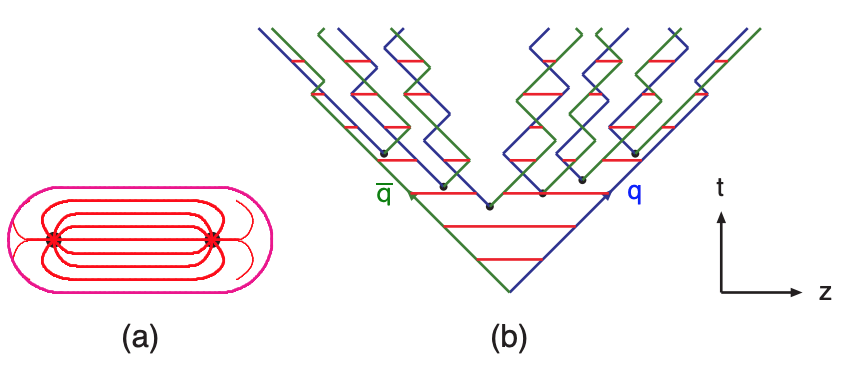
\includegraphics[width=0.6\textwidth]{figures/Simulation/StringHadronization.png}
  \caption[Illustration of hadronization in the string model]{
    Illustration of hadronization in the string model. Field
    lines from gluon exchange lead to a string-like linear force
    between $\Pq\Paq$ pairs (a). As the energy of the string increases,
    it is energetically favorable to produce new $\Pq'\Paq'$ pairs (b).
        }
 \label{fig:factorization}
\end{figure}

The cluster and string models both require input parameters derived from 
data, especially from measurements of jet formation in \EE collisions at LEP.
The string model of \PYTHIA is often seen to perform slightly better, however,
it is dependent on a greater number of parameters derived from data.
Good agreement is seen between these models for the \WZjj state considered in this analysis.
The simulation of the parton shower
and matrix element merging, discussed in the previous section, 
have significantly more impact on the dijet kinematics of the 
\WZjj state than does hadronziation process, which is most relevant to this work.

Multi-parton interactions (MPI) and pileup are also important for 
realistic picture of particle formation in LHC collisions. The MPI is primarily
soft. It does not generally result in easily identifiable jets, but
it impacts the total energy transfer in a scatter event and affects the color
connections of the scatter partons and proton remanants, leading to a more complex
hadronization stage~\cite{Buckley:2011ms}. The MPI is modeled in \Pythia, with parameters tuned 
by the CMS experiment using 7 and 8\TeV data as presented in Ref.~\cite{Khachatryan:2015pea},
referred to as the CUEP8M1 tune. Pileup is simulated using large datasets of 
events of elastic and low-energy transfer \pp scattering events, referred
to as mimimum bias events, simulated with \PYTHIA 8. Events are sampled randomly
from the dataset and mixed into the simulated sample of hard-scattering events
at with a distribution matching the number of pileup events observed in data.

Hadron decays are simulated with a combination of theoretical models,
including simple matrix element calculations for the light mesons and tau,
and observational data from experimental measurements as tabulated
by the Particle Data Group in Ref.~\ref{Tanabashi:2018oca}. Spin-dependent
decays depend on the production mechanism of the particle. 
The production and decay spin correlations are taken into account by using \textsc{MadSpin}~\cite{Artoisenet:2012st} 
together with \PYTHIA for simulations used in this analysis.

\subsection{Detector simulation}

To build a dataset of realistic collision events, used to guide this
analysis and model expected signal and background distributions,
the interactions of the particles that reach
the CMS detector in the active and inactive volume are simulated using a
detailed model in the \GEANTfour program~\cite{GEANT,Geant2}.
The paths of primary and secondary particles through the detector
\GEANTfour includes a large set of physics models over an energy range
from eV to TeV, and it effectively serves as a repository of the known
set of interactions of particles with matter.
The paths of primary particles and secondary particles through the CMS detector
are traced by \GEANTfour, using the MC method to determine interactions
according to their probabilities. Decays of semi-stable particles 
are calculated and their decay products are tracked. Energy deposits
and hits in the detector are recorded and transmitted to customized digitization software.
The digitized information, designed to accurately emulate the real CMS 
electronics, is fed through the same reconstruction algorithms as real data. 

The performance
of the detector modeling and digitization have been tuned and validated using
both test beam~\cite{CMS-DP-2018-045} and collision data~\cite{Banerjee:1345317}.
Nonetheless, differences in the simulated and collected data are unavoidable. They 
arise due to e.g., inactive regions in the detector, shifts in the detector alignment,
and radiation damage. Differences in data and simulation efficiencies are corrected
using known quantities, such as the lepton kinematics from $\cPZ$ decays or jet
energies in dijet events. These corrections are generally at the percent level. As discussed
in Chapters~\ref{ch:analysis} and \ref{ch:results}, the agreement between data
and MC simulation is excellent for most processes considered in this result.

\section{Simulations of \WZjj production}

The primary generators used in this analysis are \MG and \POWHEG 2.0 for simulation
of the hard-scattering interaction at LO or NLO, and \PYTHIA 8 for parton
showering and hadronization. The specific samples used for background processes
are discussed in Chapter~\ref{ch:analysis}. Because the MC simulations are fudamental
to distinguishing the EW- and QCD-induced contributions to \WZjj, particular
care is taken in studying the simulation of these processes.

Standard techniques to evaluate the uncertainties of MC simulations involve
varying the parameters of the PDF fit and the scale of the \muF and \muR parameters,
as discussed in Chapter~\ref{ch:analysis}. 
%Because \muF and \muR arise due to the truncation
%Of the perturbation series and the division between hard and soft scales,
%They can also be used as a probe of the impact of these choices on the calculation.
It is well established that these approaches offer a probe of the precision
of a perturbative calculation. However, the extent to which they represent
an uncertainty that can be interpreted in a statistical sense, and that fully
covers the impacts of additional missing orders of the calculation, are unknown.
In addition, additional parameters in a full simulation, such as the tuning
of the shower and hadronization to data, are not captured by this approach.
Even for fixed-order calculations, several parameters must be input to the calcultion,
including the functional form of the \muF and \muR, the couplings, and particle masses, and
widths. 

A useful approach to obtain a broad picture of the uncertainty of theoretical
predictions for a process is to compare results between different calculations.
In principle, all difference should be traceable to specific choices in the calculations.
However, probing all possible sources of differences in a hadronized prediction is a very
tedious process. It is essential when understanding sources of disagreement, but
may not be necessary when demonstrating that broadly different models of, e.g., parton
shower and hadronization, give similar results.
For the work presented in this thesis, we use comparisons of MC generators to demonstrate that the 
features of the \EWWZ and \QCDWZ processes that we exploit for this analysis 
are theoretically well understood.
Much of this work was performed
in collaboration with experts in the theoretical community at the Les Houches 2017
workshop, and reported in Ref.~\cite{leshouches2017}.

Following this work, results are presented for the following event selection,
referred to as the fiducial region.

\begin{itemize}
\item All charged leptons are required to have
    \begin{align}
        \label{cut:1}
         \pt^{\ell} >  20\GeV,\qquad |y_{\ell}| < 2.5.
    \end{align}
\item For the leptons of opposite charge and same flavour, an invariant mass cut to single out the Z-boson resonance is applied:
    \begin{align}
        \label{cut:2}
         76\GeV < m_{\ell^{+}\ell^{-}} < 106\GeV.
    \end{align}

\item hadronic or partic particles are cluster into jets using the anti-$k_T$ algorithm~\cite{Cacciari:2008gp} with radius parameter $R=0.4$.
      At least two jets are required to have
        \begin{align}
        \label{cut:3}
         \pt^{\jet} >  30\GeV, \qquad |y_{\rm j}| < 4.7, \qquad \Delta R_{\jet \ell} > 0.4,
        \end{align}
        %
        and are called tagging jets.
\item On the two leading tagging jets, typical VBS cuts are applied:
        \begin{align}
        \label{cut:4}
        \mjj >  500\GeV,\qquad \abs{\detajj} > 2.5.
        \end{align}
\end{itemize}
\subsection{Predictions from fixed-order calculations}

Calculations of the \EWWZ process at NLO in QCD were first performed
some over ten years ago~\cite{Bozzi:2007ur}, however, only recently have these
results been implemented in a form that is compatible with parton shower and 
hadronization generators~\cite{Jager:2018cyo}. Recent preliminary
results considering both NLO EW and QCD effects for \WZjj production are also limited to fixed order.
Therefore, it is necessary to consider fixed-order results when considering
the best available predictions for this process. The additional
complications of showered and hadronized events can complicate efforts to
establish the relative agreement of generators. 

\begin{figure}[htbp]
  \centering
   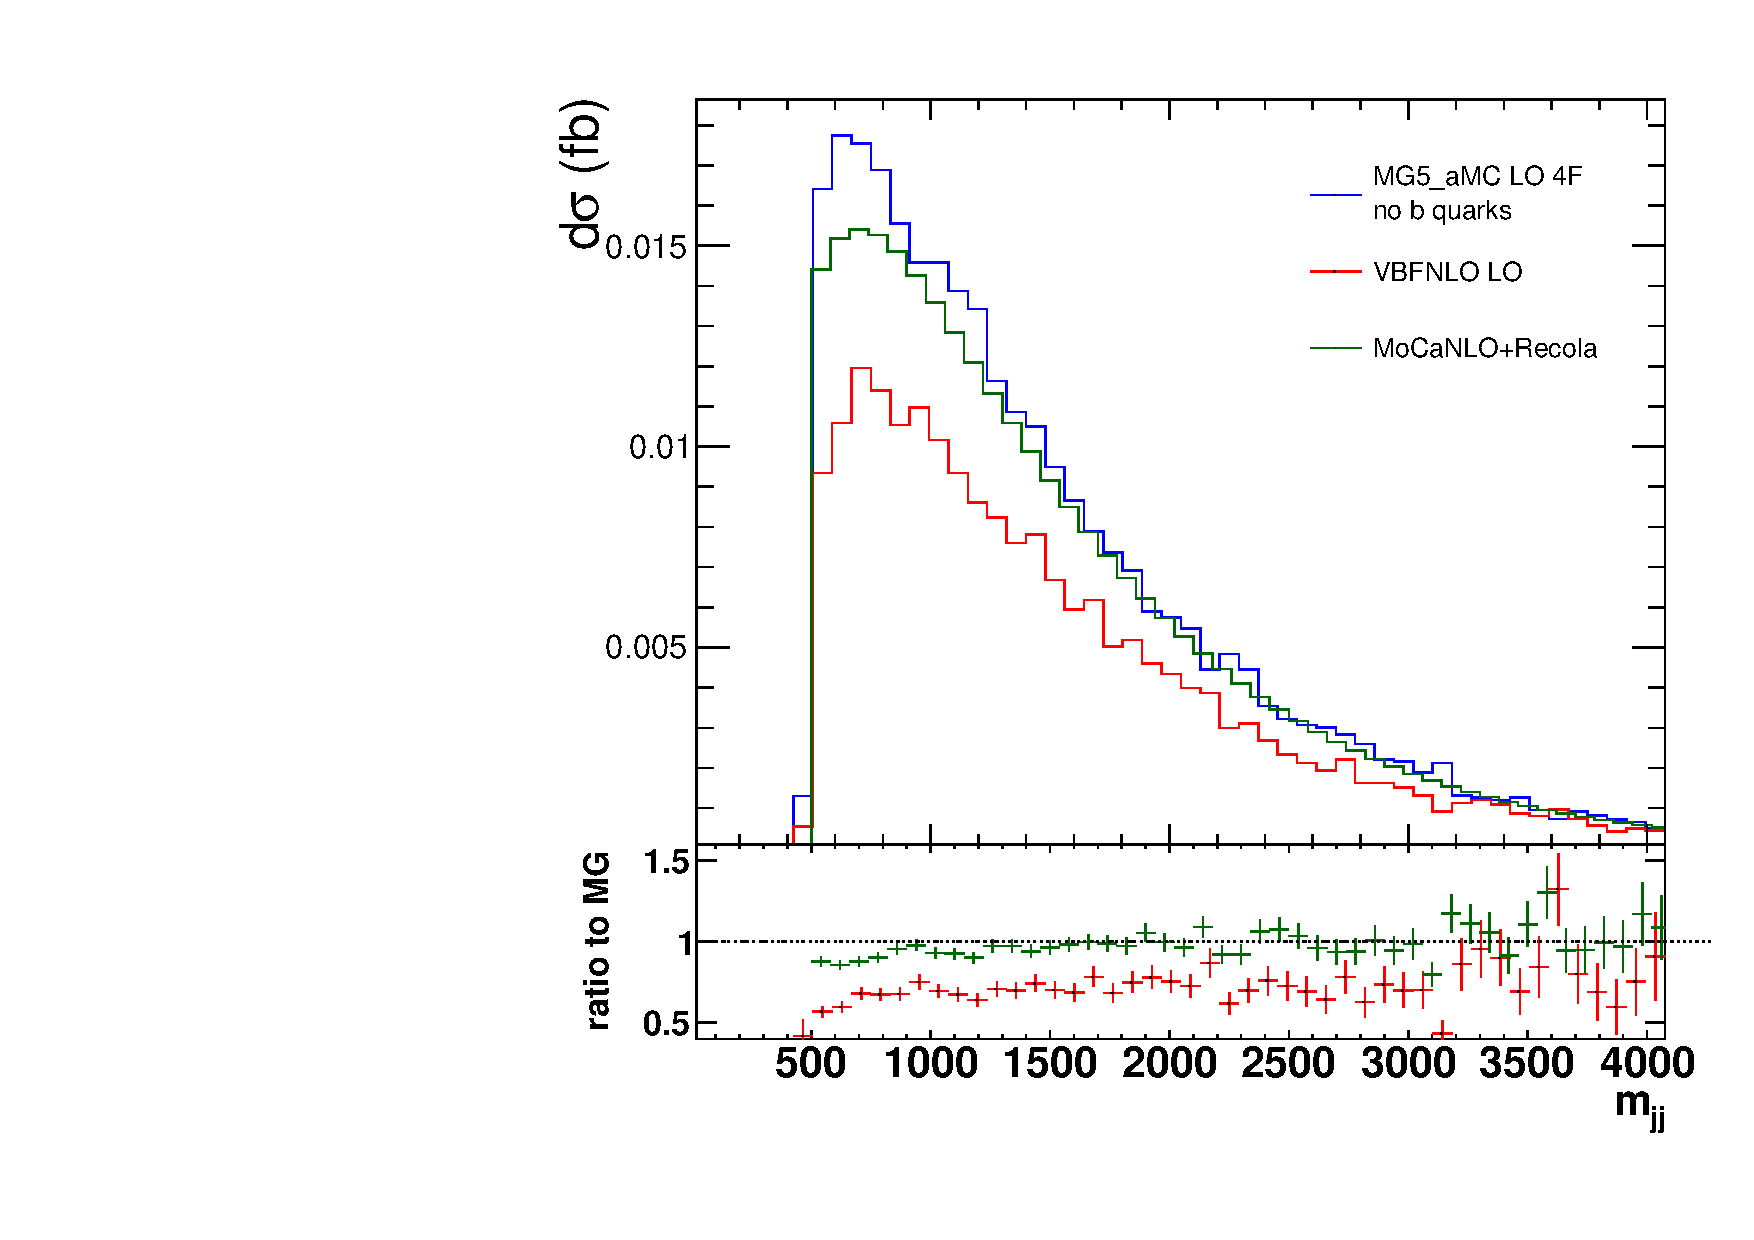
\includegraphics[width=0.49\textwidth]{figures/Simulation/mjj_FO_untuned.pdf}
   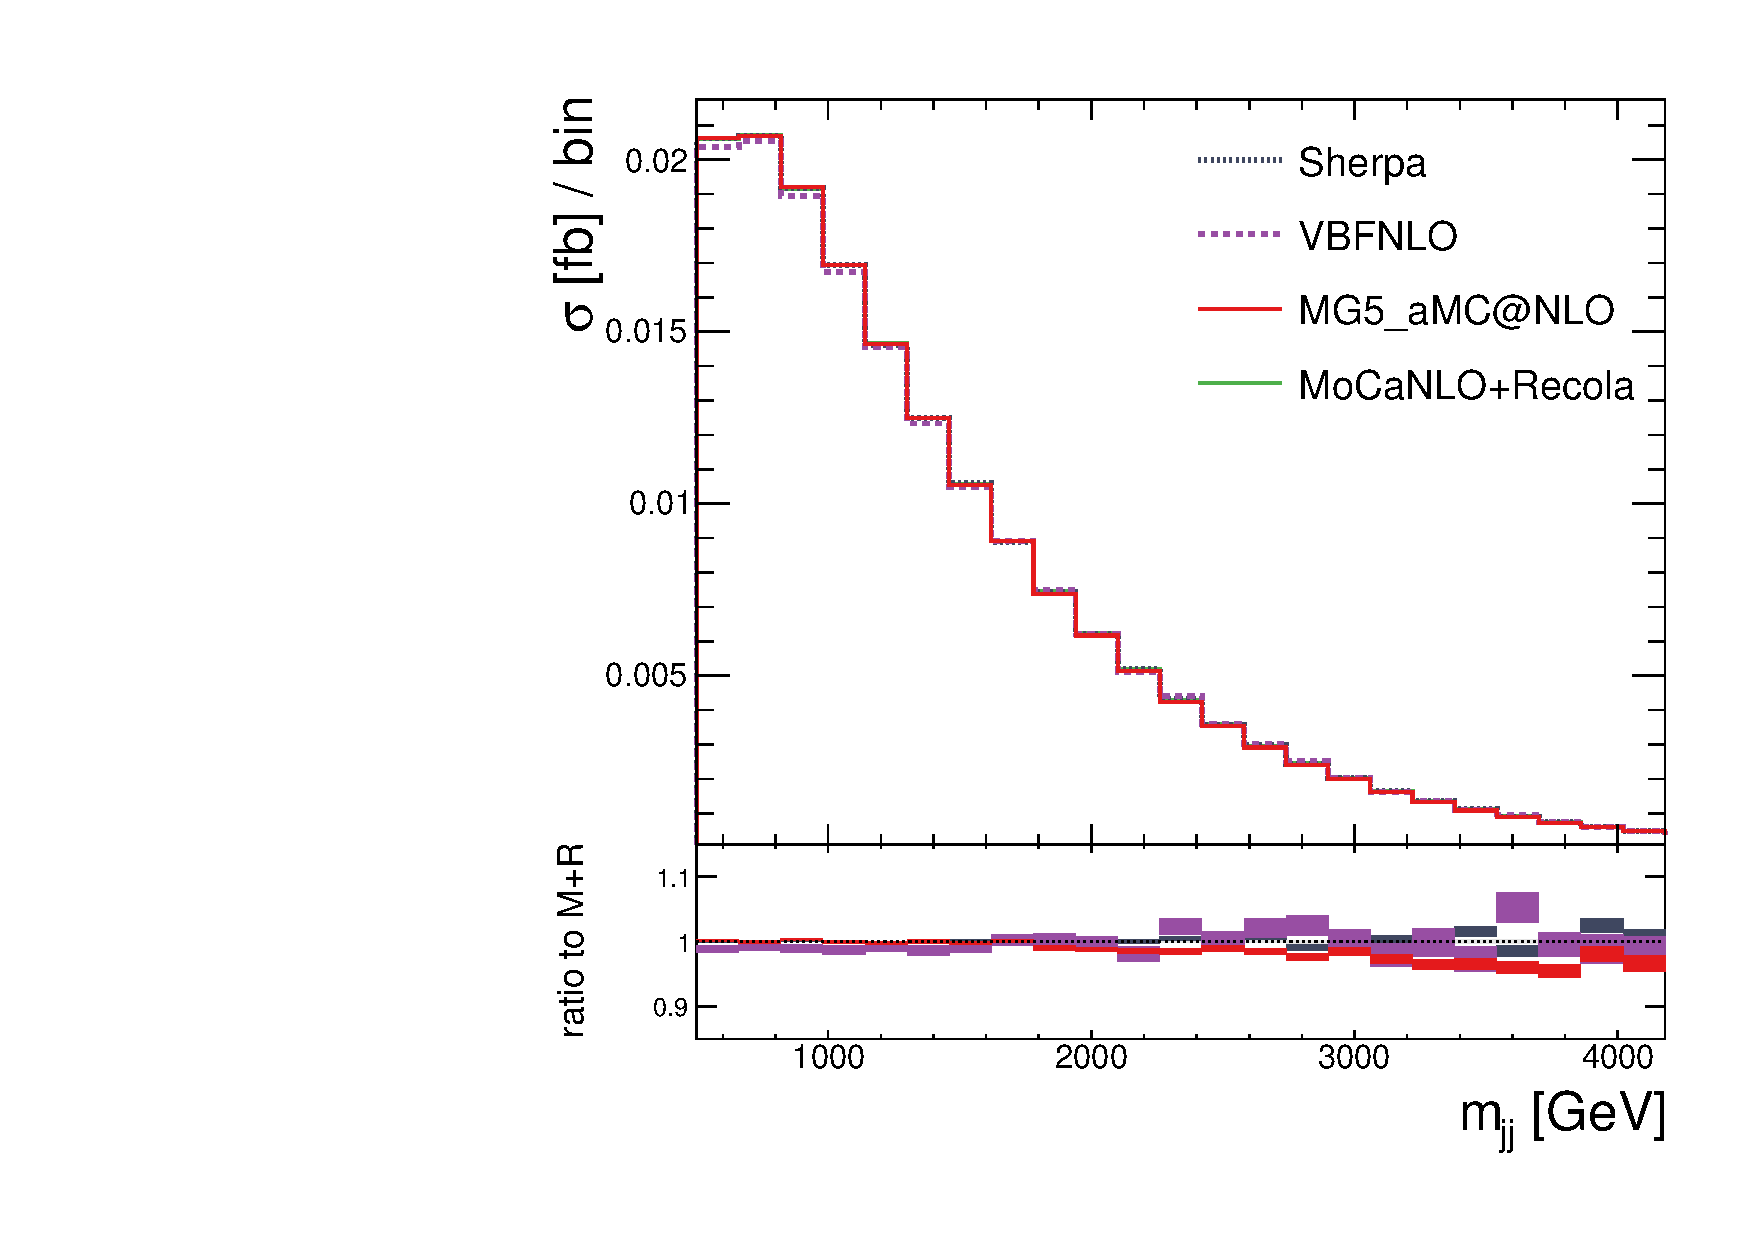
\includegraphics[width=0.49\textwidth]{figures/Simulation/mjj_FO_tuned.pdf}
  \caption[The fixed-order prediction for $\mjj$ from \MG, \Sherpa, \VBFNLO, and \Moca at LO]
  {
    The fixed-order prediction for $\mjj$ from \MG, \Sherpa, \VBFNLO, and \Moca at LO
    for the \EWWZ process. The left plot shows comparisons using the default settings
    of all input parameters for the public MC programs. The right plot is shown
    with parameters tuned to the values given in Ref.~\cite{leshouches2017}.
        }
 \label{fig:FOWZcomparisons}
\end{figure}

For this reason, we first consider comparisons of the \EWWZ process at fixed order. 
Because the process has no $\alpha_s$ couplings at LO, the 
calculation has almost no $\muR$ dependence.
The $\muR$ dependence is also relatively low, $\mathcal{O}(10\%)$
leading order. Furthermore, the NLO corrections to the cross section are small,
the $k$-factor $k\def \sigma_{NLO}/\sigma_{LO} = 0.98$ in the fiducial region
defined in Equations~\ref{eq:cut1}-\ref{eq:cut4}, calculated with 
VBFNLO~\cite{VBFNLO}. Nonetheless, the process has a significant dependence on
the masses, widths, and couplings of the particles used in the calculation,
as demonstrated in Fig.~\ref{fig:FOWZcomparisons}. The Les Houches study demonstrated
that discrepancies may arise at fixed-order when these parameters are not controlled,
however, when using a common, adjusted to the best-available measurements and
well-motivated parameters, excellent agreement is obtained. 
Because most settings can be determined in an objective way, we do not consider
differences to constitute additional uncertainty in modeling this process.

\subsection{Hadronized predictions and fully-simulated events}

We also study the modeling of the \EWWZ process using hadronized events. 
The results are largely consistent with the studies at fixed order;
agreement is seen across a broad range of generators for leptonic variables,
or kinematic variables of the two jet system. 
Specifically, the variables $\mjj$, $\etajj$, and
$\etas \def \zepl$ (sometimes referred to as the "Zeppenfeld variable") are
all well described, and can be exploited in this analysis with limited uncertainty.
Variables depending on more than
three clustered jets are produced purely by the shower and hadronization
can have significant differences. This is expected: the parton shower and hadronization
of \Sherpa, \Herwig, \MG, and \Pythia use different models and different tuned parameters.
Because many are phenomenological nature, it is difficult to constrain them extensively.
We acknowledge a higher modeling uncertainty for such variables, and seek to avoid
relying on their simulation in this analysis. Example distributions with large
and small shower dependence are shown in Fig.~\ref{fig:ewwzHadronization}.

\begin{figure}[htbp]
  \centering
   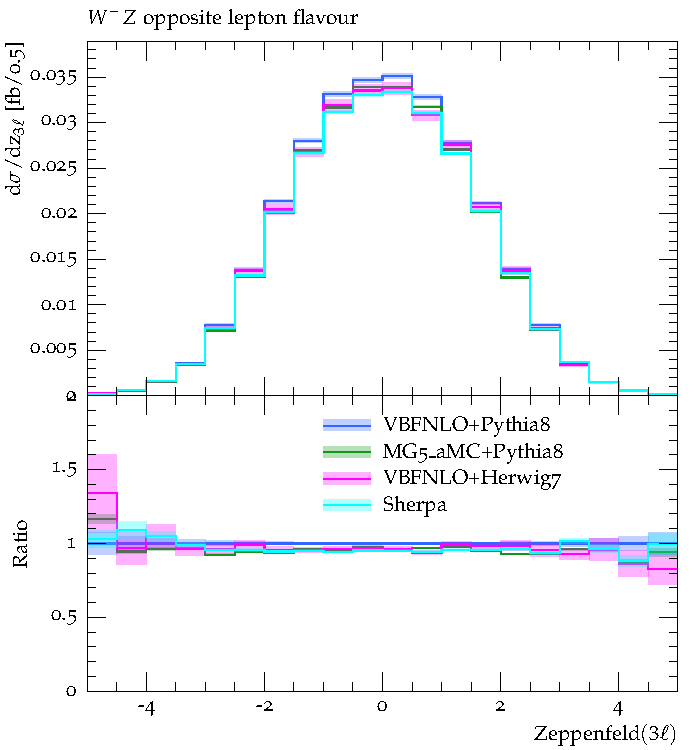
\includegraphics[width=0.49\textwidth]{figures/Simulation/LH_VBFNLO_WmZ_OF_zep3l.pdf}
   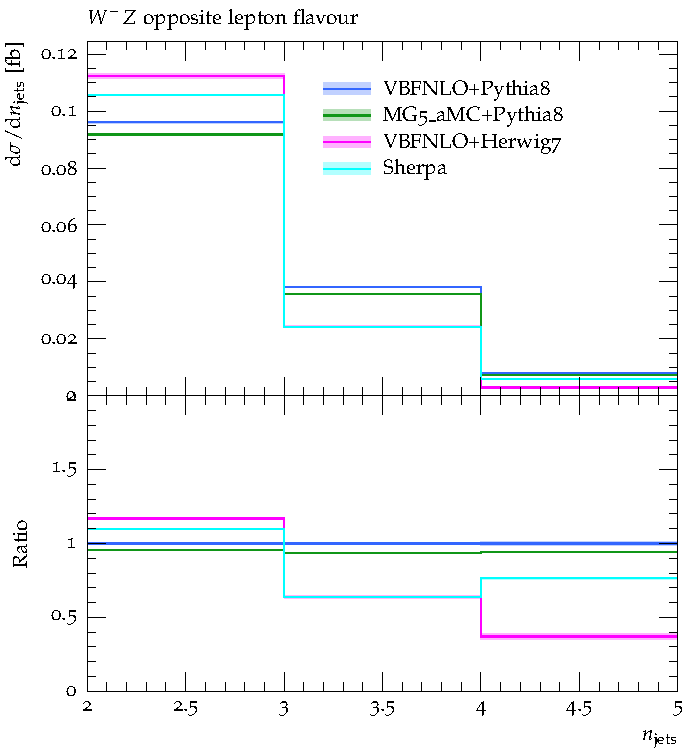
\includegraphics[width=0.49\textwidth]{figures/Simulation/LH_VBFNLO_WmZ_OF_nJets.pdf}
  \caption[Comparison of predictions for \EWWZ production including hadronization effects]
  {
    Predictions for EW $\PW^{-}\cPZ\to\EE\mu\nu_{\mu}$ production, including the parton
    shower and hardonization. Variables well-described by the fixed-order calculation,
    including $\etas$ (left), are not significantly impacted by the shower and hadronization.
    Variables with a large dependence on shower and hadronization, including the number
    of cluster jets with $\pt > 30\GeV$ (right), shower larger variance between MC generators.
        }
 \label{fig:ewwzHadronization}
\end{figure}

Because QCD-induced \WZjj production is $\mathcal{O}(\alpha_s^{2})$ it has a large
dependence on $\muF$ and $\muR$, especially at LO. Fixed order predictions

\chapter{Event reconstruction}
\label{ch:reconstruction}
\section{Global event description via particle flow}
  \subsection{Tracks and vertices}
  \subsection{Calorimeter clusters}
  \subsection{Particle flow candidates}
\section{Physics objects}
  \subsection{Muons}
  \subsection{Electrons}
  \subsection{Charged and neutral hadrons}
  \subsection{Jets}
  \subsection{Identification b-jets}
  \subsection{Missing transverse momentum}


\chapter{Analysis Strategy}

\section{WZ VBS event signature and background composition}
\section{Event triggering}
\section{Event selection}
\subsection{WZjj cross section, EW WZ and aQGC search}
\subsection{Charged Higgs boson search}
\section{Background contributions}
\subsection{Estimation of nonprompt backgrounds}
\subsection{Simulation and validation of prompt backgrounds}
\section{Statistical procedures}
\subsection{WZjj cross section measurement}
\subsection{Significance of electroweak WZ Production}
\subsection{Limits on charged Higgs bosons}
\subsection{Limits on anomalous quartic gauge couplings}
\section{Systematic uncertainties}

\begin{table}[!ht]
  \begin{center}
  \caption{Summary of event selections and fiducial region definitions for the analysis. 
    The selections labeled ``EW signal'' and ``Higgs boson'' are applied to data and reconstructed 
    simulated events.
    The EW signal selection is used for all measurements except for charged the charged Higgs boson search,
    which uses the selection indicated in the column labeled ``Higgs boson''.
    The \WZjj cross section is reported in the fiducial regions defined by the selections specified in 
    the last two columns, which are applied to simulated events.
    $n_{\jet}$, $n_{\mathrm{b}}$, and $\pt^{\mathrm{b}}$ refer to the number of
    anti-\kt jets, the number of anti-\kt b-tagged jets, and the b jet 
    \pt threshold, respectively. Other variables are defined in the text.
    }
  \begin{tabular}{c|c|c|c|c}
  \hline
                                    & EW signal & Higgs boson & Tight fiducial & Loose fiducial\\
    \hline\hline
    $  \PT^{\ell'_{1}}   $ [GeV]    & $> 25$    & $> 25$        & $ > 25 $       & $ > 20 $ \\
    $  \PT^{\ell'_{2}}   $ [GeV]    & $> 15$    & $> 15$        & $ > 15 $       & $ > 20 $ \\
    $  \PT^{\ell}     $ [GeV]       & $> 20$    & $> 20$        & $ > 20 $       & $ > 20 $ \\
  $\left|\eta^{\mu}\right|   $      & $< 2.4$   & $< 2.4$       & $ < 2.5$       & $ < 2.5$ \\
    $\left|\eta^{\mathrm{e}}\right|$      & $< 2.5$   & $< 2.5$       & $ < 2.5$       & $ < 2.5$ \\
  $\left|m_{\ell'\ell'}-m_{\Z}\right|$ [GeV] & $ < 15 $ & $ < 15 $ & $ < 15 $ & $ < 15 $ \\
  $m_{3\ell}                $ [GeV] & $> 100$   & $> 100$       & $> 100$        & $> 100$    \\
  $m_{\ell\ell}           $ [GeV]   & $> 4$     & $> 4$         & $>4$           & $>4$    \\
  $\ptmiss                  $ [GeV] & $> 30$       & $> 30$     &   -            &   -     \\
  $\left|\eta^{\jet}\right|  $      & $< 4.7$   & $< 4.7$       & $< 4.7$        & $< 4.7$ \\
    $\PT^{\jet}                $ [GeV] & $ > 50$   & $> 30$        & $> 50$         & $> 30$  \\
  $\left|\Delta R(\jet, \ell)\right|$            & $ > 0.4$  & $> 0.4$       & $> 0.4$        & $> 0.4$ \\
  $n_{\mathrm{\jet}}           $    & $\ge 2$   & $\ge 2$       & $\ge 2$        & $\ge 2$    \\
  $\PT^{\mathrm{b}}         $ [GeV] & $ > 30$   & $ > 30$       &   -            &   -     \\
  $n_{\mathrm{b}}       $         & $= 0$     & $= 0$         &   -            &   -     \\
  $\mjj             $               & $> 500$   & $> 500$       & $> 500$        & $> 500$ \\
  $\left|\etajj \right|$            &$> 2.5$         & $> 2.5$ & $> 2.5$ & $> 2.5$ \\
  $\left| \zepl \right|$            & $< 2.5$ & - & $< 2.5$ & - \\
  \end{tabular}
  \label{tab:selections}
  \end{center}
\end{table}


\begin{table}[htbp]
     \centering
     \caption{ The dominant uncertainty contributions in the fiducial 
         \WZjj cross section measurement 
         and their expected contributions to the significance of the
         \EWWZ signal strength measurement. The impact of each systematic 
         uncertainty in the \WZjj 
         cross section measurement is obtained by freezing the set of associated nuisance 
         parameters to their best fit values and comparing the total uncertainty in the signal strength
         to the result from the nominal fit. 
         The effect on the \EWWZ significance, shown in the last column,
         is defined as the relative increase in the expected significance when
         freezing the nuisance term to its best fit value.
           }
     \begin{tabular}{l|ccc}
 \hline %------------------------------------------------------------------------------------------
     Source of systematic uncertainty & \multicolumn{3}{c}{Relative systematic uncertainty [\%]} \\
                                      & $\sigma_{\WZjj}$ & \EWWZ significance \\
 \hline %------------------------------------------------------------------------------------------
 \hline %------------------------------------------------------------------------------------------
 Jet energy scale                     & $+10.7\, /-8.1$ & $ 7.0 $               \\ %done
 Jet energy resolution                & $+1.9\,/-2.1$   & $< 0.1$             \\ %done
 \QCDWZ modeling                      &    N/A          & $ 2.2 $             \\
 Other background theory              &  $+2.2\,/-2.2$  & $ 0.3 $             \\ %done
 Nonprompt normalization              &  $+2.5\,/-2.5$  & $ 0.3 $             \\ %done
 Nonprompt event count                &  $+6.0\,/-5.8$  & $ 1.7 $               \\ %done
 Lepton energy scale and eff.         &  $+3.5\,/-2.7$  & $< 0.1$             \\ %done
 b tagging                            &  $+2.0\,/-1.7$  & $< 0.1$             \\ %done
 Integrated luminosity                &  $+3.6\,/-3.0$  & $< 0.1$             \\ %done
 \hline %------------------------------------------------------------------------------------------
      \end{tabular}
     \label{tab:systematics}
\end{table}


\begin{table}[htbp]
     \centering
     \caption{ The dominant uncertainty contributions in the fiducial 
         \WZjj cross section measurement 
         and their expected contributions to the significance of the
         \EWWZ signal strength measurement. The impact of each systematic 
         uncertainty in the \WZjj 
         cross section measurement is obtained by freezing the set of associated nuisance 
         parameters to their best fit values and comparing the total uncertainty in the signal strength
         to the result from the nominal fit. 
         The effect on the \EWWZ significance, shown in the last column,
         is defined as the relative increase in the expected significance when
         freezing the nuisance term to its best fit value.
           }
     \begin{tabular}{l|cc}
 \hline %------------------------------------------------------------------------------------------
     Source of systematic uncertainty & Relative systematic uncertainty [\%] \\
                                      & $\sigma_{\rm \WZjj}$ \\
 \hline %------------------------------------------------------------------------------------------
 \hline %------------------------------------------------------------------------------------------
 Jet energy scale                     & $+10.7\, /-8.1$ &               \\ %done
 Jet energy resolution                & $+1.9\,/-2.1$   &             \\ %done
 \QCDWZ modeling                      &    N/A          &             \\
 Other background theory              &  $+2.2\,/-2.2$  &             \\ %done
 Nonprompt normalization              &  $+2.5\,/-2.5$  &             \\ %done
 Nonprompt event count                &  $+6.0\,/-5.8$  &               \\ %done
 Lepton energy scale and eff.         &  $+3.5\,/-2.7$  &             \\ %done
 b tagging                            &  $+2.0\,/-1.7$  &             \\ %done
 Integrated luminosity                &  $+3.6\,/-3.0$  &             \\ %done
 \hline %------------------------------------------------------------------------------------------
      \end{tabular}
     \label{tab:systematics}
\end{table}

\begin{table}[htbp]
     \centering
     \caption{ The dominant uncertainty contributions in the fiducial 
         \WZjj cross section measurement 
         and their expected contributions to the significance of the
         \EWWZ signal strength measurement. The impact of each systematic 
         uncertainty in the \WZjj 
         cross section measurement is obtained by freezing the set of associated nuisance 
         parameters to their best fit values and comparing the total uncertainty in the signal strength
         to the result from the nominal fit. 
         The effect on the \EWWZ significance, shown in the last column,
         is defined as the relative increase in the expected significance when
         freezing the nuisance term to its best fit value.
           }
     \begin{tabular}{l|cc}
 \hline %------------------------------------------------------------------------------------------
     Source of systematic uncertainty & Relative systematic uncertainty [\%] \\
                                      & \EWWZ significance \\
 \hline %------------------------------------------------------------------------------------------
 \hline %------------------------------------------------------------------------------------------
 Jet energy scale                     & $ 7.0 $               \\ %done
 Jet energy resolution                & $< 0.1$             \\ %done
 \QCDWZ modeling                      & $ 2.2 $             \\
 Other background theory              & $ 0.3 $             \\ %done
 Nonprompt normalization              & $ 0.3 $             \\ %done
 Nonprompt event count                & $ 1.7 $               \\ %done
 Lepton energy scale and eff.         & $< 0.1$             \\ %done
 b tagging                            & $< 0.1$             \\ %done
 Integrated luminosity                & $< 0.1$             \\ %done
 \hline %------------------------------------------------------------------------------------------
      \end{tabular}
     \label{tab:systematics}
\end{table}

\chapter{Results}

\section{Fiducial WZjj cross section measurement}

The cross section for \WZjj production, without separating by production mechanism,
is measured with a combined maximum likelihood fit to the 
observed event yields.
The likelihood is a combination of individual likelihoods for the four decay channels for the
signal and background hypotheses with the statistical and systematic uncertainties in the form
of nuisance parameters. 
The expected event yields for the EW- and QCD-induced \WZjj processes
are taken from the \MG~v2.4.2 predictions. 
A signal strength $\mu_{\WZjj}$, which represents the 
ratio of the measured signal yield to the expected number of signal events, 
is treated as a free parameter in the fit.

\begin{figure}[htbp]
  \centering
   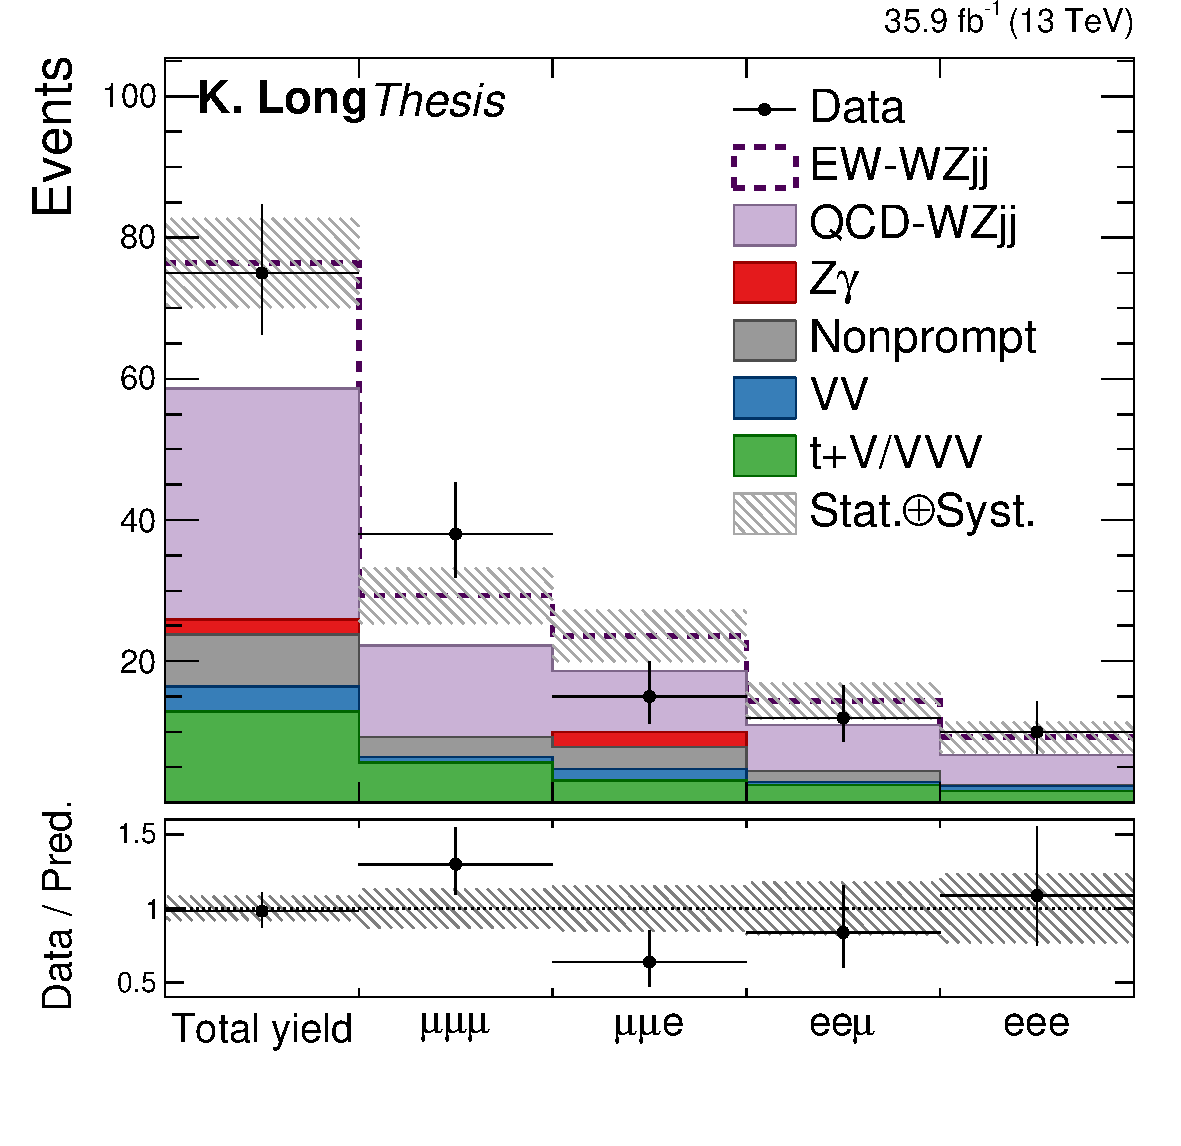
\includegraphics[width=0.7\textwidth]{figures/AnalysisResults/yieldByChannel.pdf}
  \caption{
    Post fit event yields in the EW signal region.
          }
 \label{fig:EWSignalYields}
\end{figure}

The best fit value for the signal strength is used to obtain a cross section
in the tight fiducial region defined in Table~\ref{tab:selections}. 
The measured fiducial \WZjj cross section in this region is

\begin{equation}
  \sigma^{\mathrm{fid}}_{\mathrm{WZjj}} = 
        3.18^{+0.57}_{-0.52} \, \mathrm{(stat)} \,\, ^{+0.43}_{-0.36} \, \mathrm{(syst)}
        = 3.18^{+0.71}_{-0.63} \,\unit{fb} \,.
\end{equation}

This result can be compared to the predicted value of
$3.27 \, ^{+0.39}_{-0.32} \mathrm{(scale)} \pm 0.15\, \mathrm{(PDF)} \unit{fb}$.
The \EWWZ and \QCDWZ contributions are
calculated independently from the samples described in Section~\ref{sec:mc}
and their uncertainties are combined in quadrature. 
The interference term contribution in this region is less than 1\% of
the total cross section.

Results are also obtained in a looser fiducial region, defined in Table~\ref{tab:selections}
following Ref.~\cite{leshouches2017},
to simplify comparisons with theoretical calculations.
The acceptance from the loose to tight fiducial region
is $(72.4 \pm 0.8)\%$,
computed using \MG interfaced to \PYTHIA. 
The uncertainty in the acceptance is evaluated independently 
for the \EWWZ and \QCDWZ samples
from the scale
and PDF uncertainties, which are combined in quadrature.
The scale uncertainty in the \QCDWZ contribution is the 
dominant component of the uncertainty.
The resulting \WZjj loose fiducial cross section is

\begin{equation}
  \sigma^{\mathrm{fid, loose}}_{\mathrm{WZjj}} = 
        4.39^{+0.78}_{-0.72} \, \mathrm{(stat)} \,\, ^{+0.60}_{-0.50} \, \mathrm{(syst)}
        = 4.39^{+0.98}_{-0.87} \,\unit{fb} \,,
\end{equation}

which can be compared to the predicted value of 
$4.51^{+0.59}_{-0.45} \, \mathrm{(scale)} \pm 0.18 \, \mathrm{(PDF)} \unit{fb}$.
The \EWWZ and \QCDWZ contributions 
and their uncertainties are treated independently with the same approach as described
for the tight fiducial region.

\section{Search for EW WZ boson production}

\begin{figure}[htbp]
  \centering
   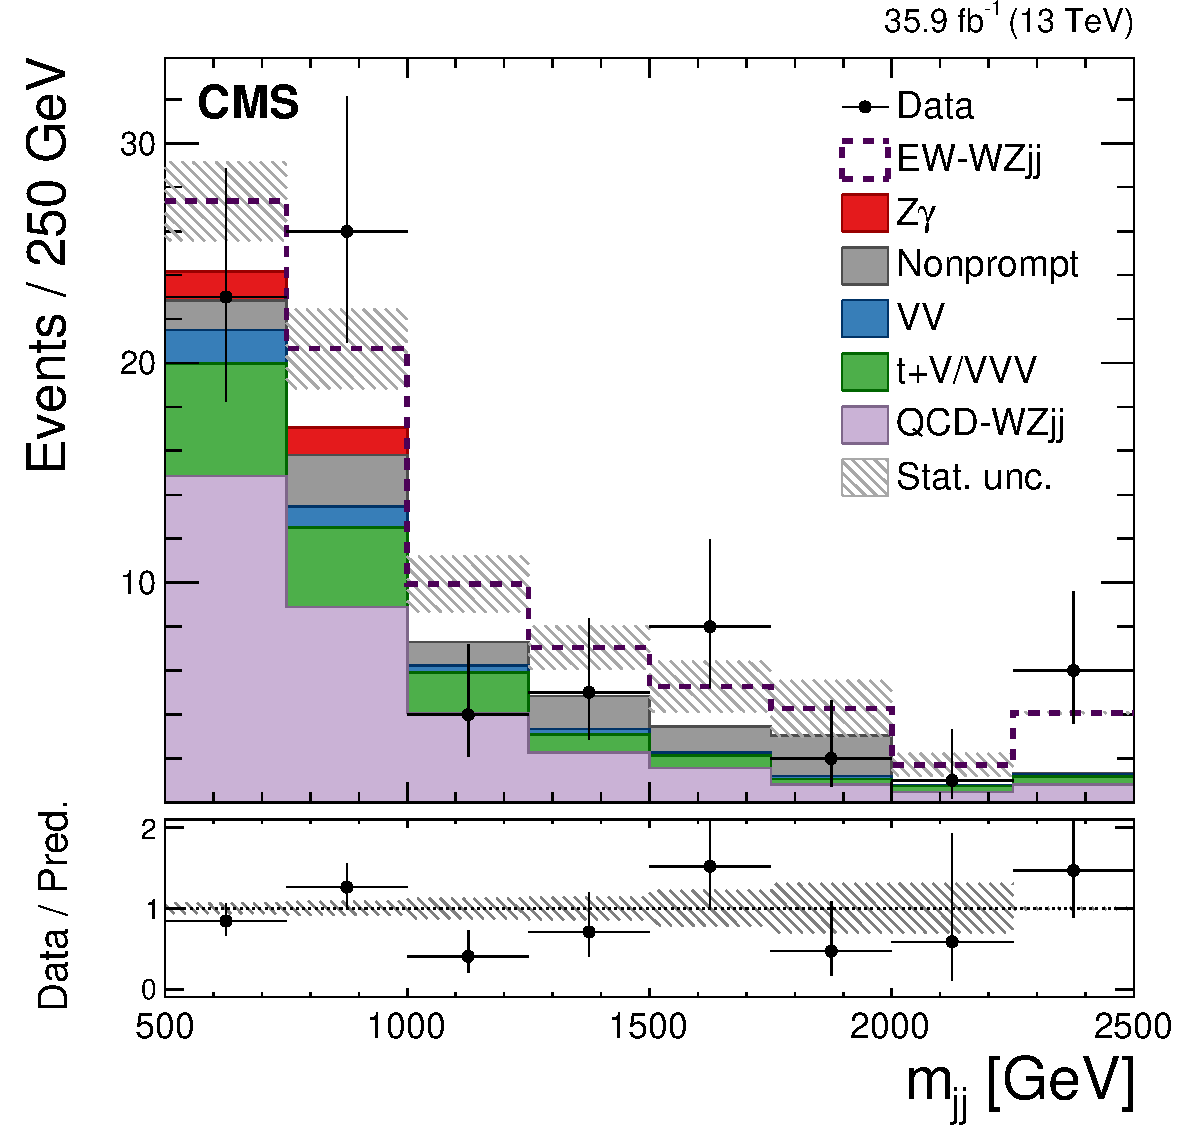
\includegraphics[width=0.45\textwidth]{figures/AnalysisResults/mjj.pdf}
   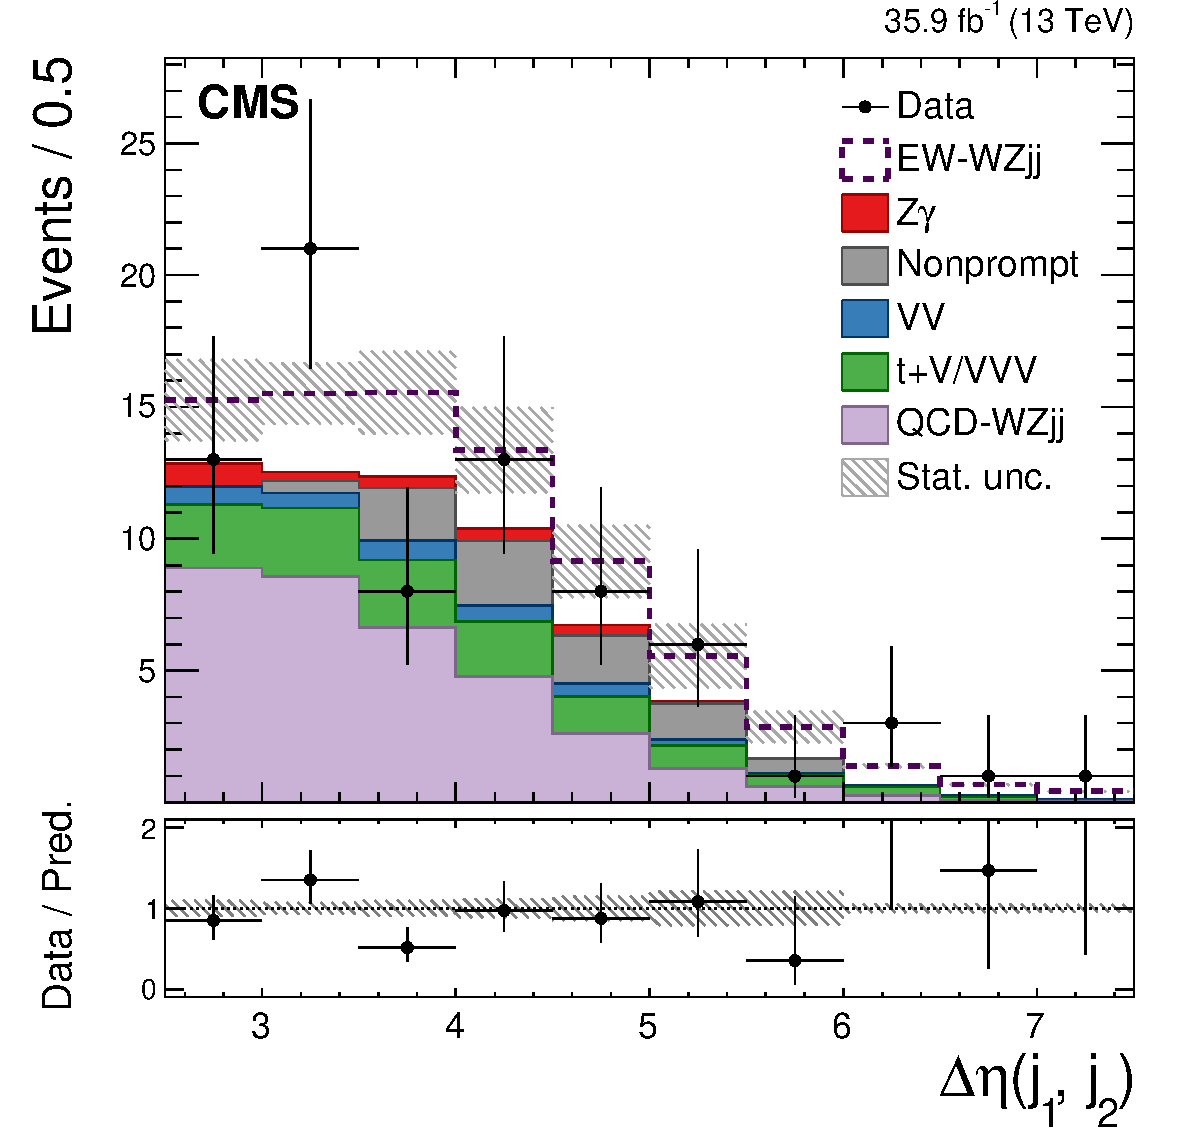
\includegraphics[width=0.45\textwidth]{figures/AnalysisResults/dEtajj.pdf}
  \caption{
  The $\mjj$ (left) and $\left|\etajj\right|$ 
  of the two leading jets 
  (right) for events satisfying the EW signal selection. 
  The last bin contains all events with $\mjj > 2500\GeV$ (left) and 
  $\left|\etajj\right| > 7.5$ (right).
  The dashed line shows the expected \EWWZ contribution stacked
  on top of the backgrounds, which are shown as filled histograms. 
  The hatched bands represent the total and relative 
  statistical uncertainties on the predicted yields.
  The bottom panel shows the ratio of the number of events measured in data to the total 
  number of expected events. 
  The predicted yields are shown with their prefit normalizations.
          }
 \label{fig:VBSPlots}
\end{figure}

\begin{figure}[htbp]
  \centering
   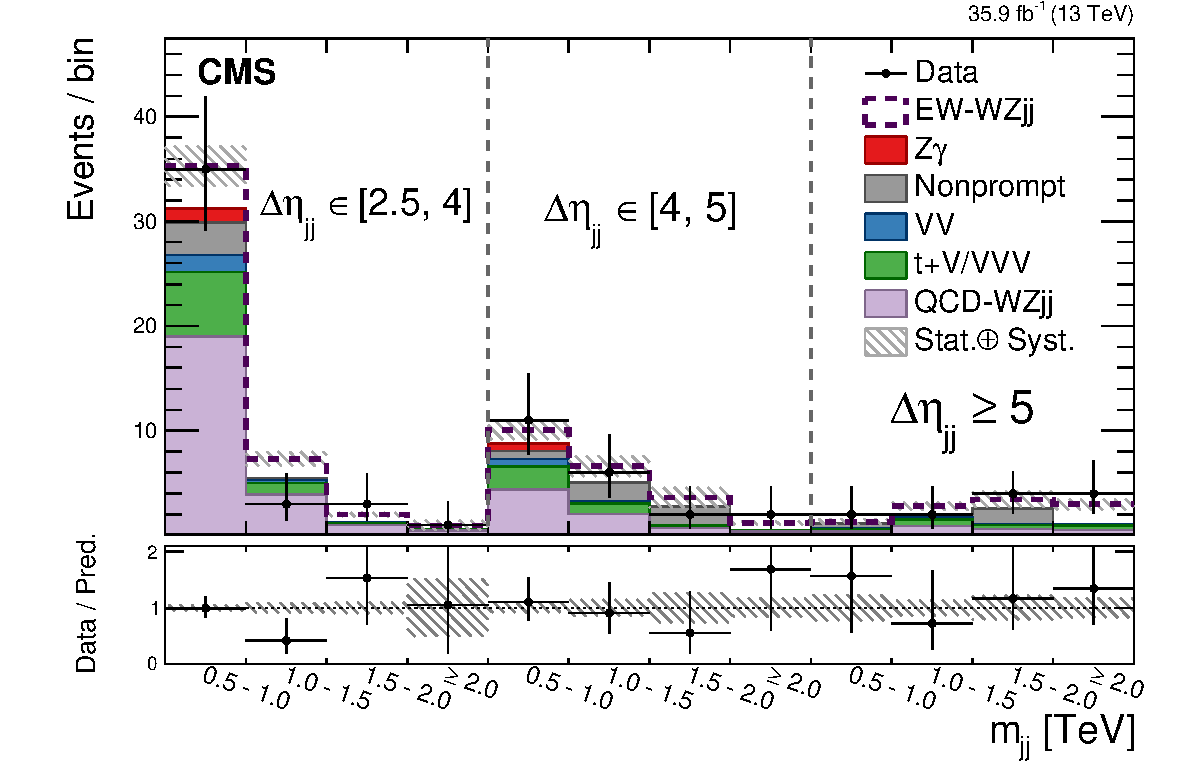
\includegraphics[width=0.7\textwidth]{figures/AnalysisResults/mjj_etajj_unrolled.pdf}
    \caption{
      The one-dimensional representation of the 2D distribution of 
      $\mjj$ and $\left|\etajj\right|$, used for the EW 
      signal extraction. The x axis shows the dijet mass distribution
      in the indicated bins, split into three bins of {\etajj }: {\etajj} $\in [2.5, 4], [4, 5], \ge 5$.
      The dashed line represents the \EWWZ contribution stacked
      on top of the backgrounds, which are shown as filled histograms. 
      The hatched bands represent the total and relative 
      systematic uncertainties on the predicted yields.
      The bottom panel shows the ratio of the number of events measured in data to the total 
      number of expected events. 
      The predicted yields are shown with their best fit normalizations.
    }
  \label{fig:2DfitDistribution}
\end{figure}
\section{New physics searches}

\subsection{Limits on anomalous quartic gauge couplings}

\begin{figure}[htbp]
  \centering
    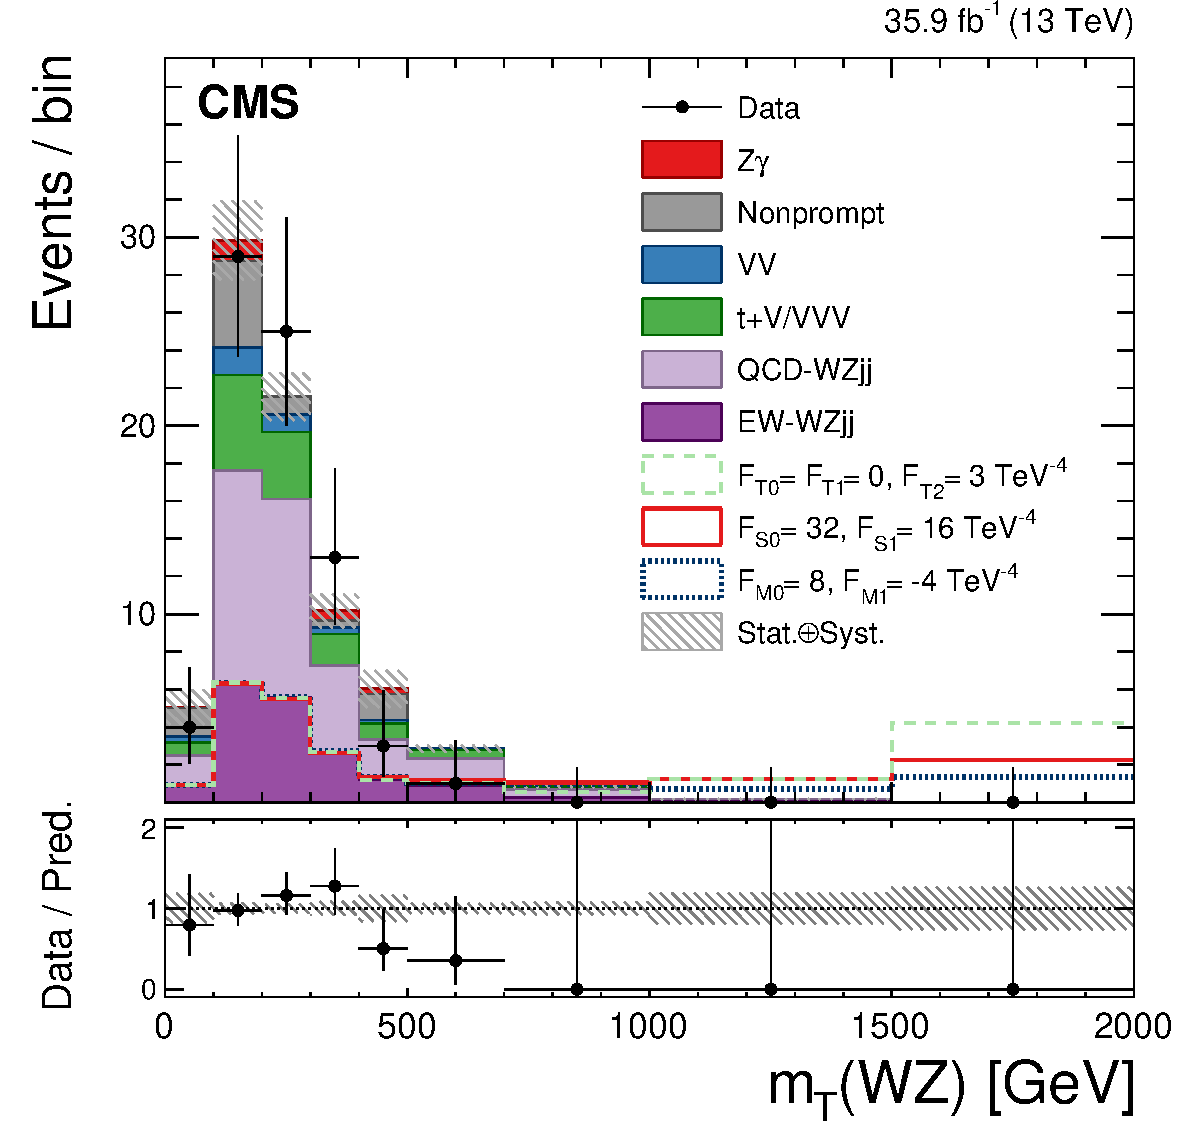
\includegraphics[width=0.5\textwidth]{figures/AnalysisResults/MTWZ_aQGC.pdf}
  \caption{
      $\mt$ for events satisfying the EW signal selection,
      used to place constraints on the anomalous coupling parameters.
      The dashed lines show predictions for several aQGC parameters values, which modify the \EWWZ process.
      The last bin contains all events with $\mt > 2000\GeV$.
      The hatched bands represent the total and relative 
      systematic uncertainties on the predicted yields.
      The bottom panel shows the ratio of the number of events measured in data to the total 
      number of expected events. 
      The predicted yields are shown with their best-fit normalizations from the background-only fit.
      }
 \label{fig:aQGCDistribution}
\end{figure}

\subsection{Limits on charged Higgs boson production}

\begin{figure}[htbp]
  \centering
   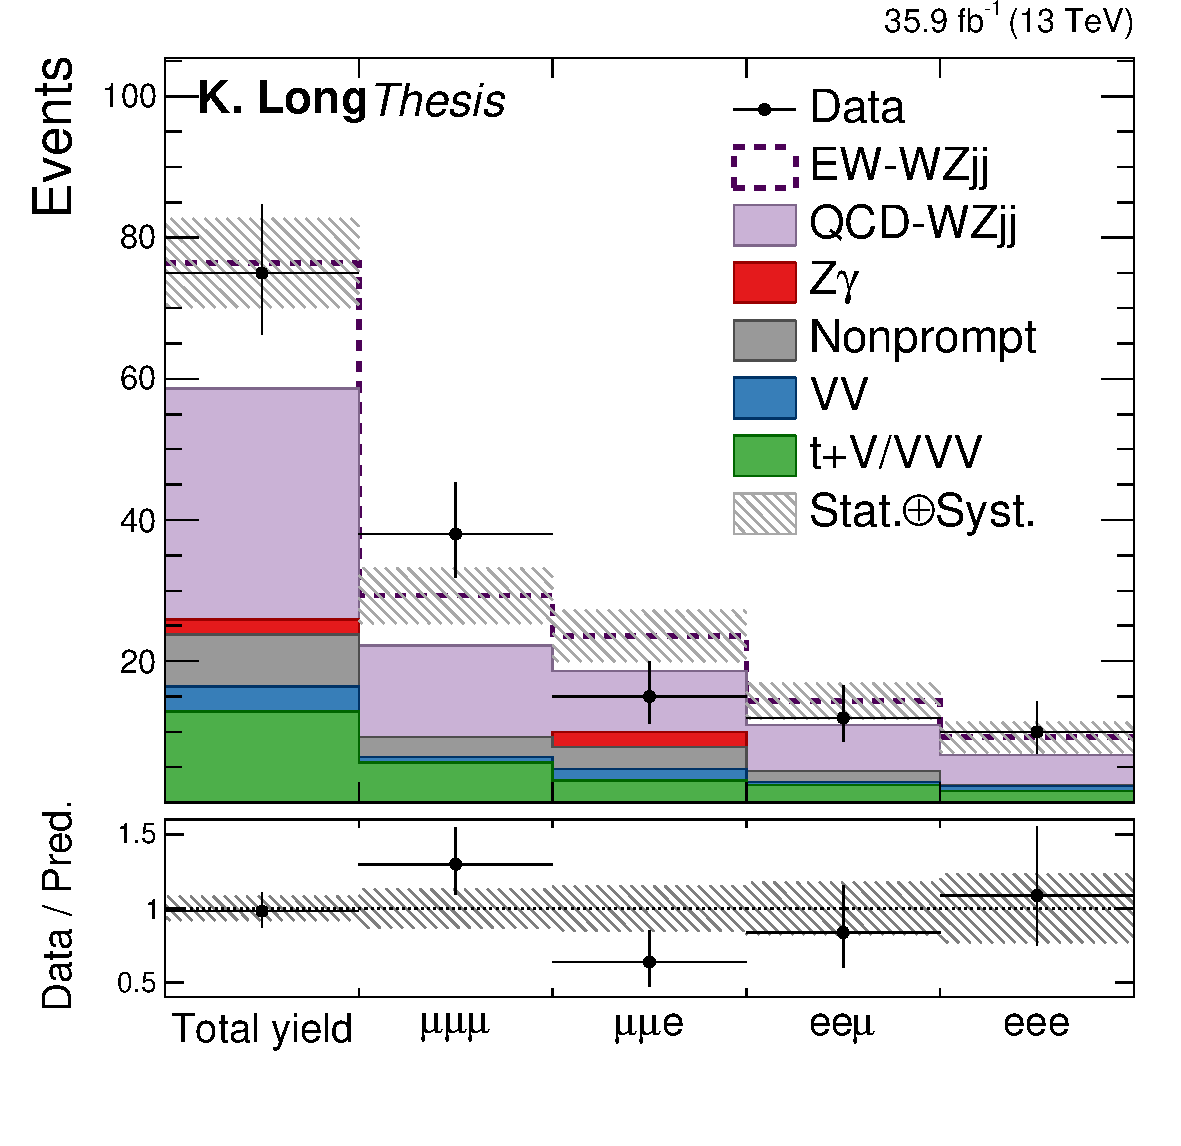
\includegraphics[width=0.7\textwidth]{figures/AnalysisResults/yieldByChannel.pdf}
  \caption{
    Post fit event yields in the charged Higgs boson search region.
          }
 \label{fig:EWSignalYields}
\end{figure}


\chapter{Conclusions}

\section{Summary}

A measurement of the production of a {\PW} and a $\PZ$ boson in association with two jets has been presented,
using events where both bosons decay leptonically.
Results are based on data corresponding to an integrated luminosity of $35.9\fbinv$
recorded in proton-proton collisions at $\sqrt{s} = 13\TeV$ with the CMS detector
at the LHC in 2016. The cross section in a tight fiducial region with enhanced contributions from
electroweak (EW) \WZ production is $\sigma^{\mathrm{fid}}_{\WZjj} = 3.18^{+0.71}_{-0.63}\unit{fb}$,
consistent with the standard model (SM) prediction.
The dijet mass and dijet rapidity separation are used to measure
the signal strength of \EWWZ production with
respect to the SM expectation, resulting in
$\mu_{\EW} = 0.82^{+0.51}_{-0.43}$.
The significance of this result is
2.2 standard deviations with 2.5 standard deviations expected.
at $13\TeV$.
This is the first study of this process performed by the CMS Collaboration.

Constraints are placed on anomalous quartic gauge couplings
in terms of dimension-eight effective field theory operators, and
upper limits are given on the production cross section
times branching fraction of charged Higgs bosons.
The upper limits on charged Higgs boson production
via vector boson fusion with decay to a {\PW} and a {\cPZ} boson
extend the results previously published
by the CMS Collaboration~\cite{Sirunyan:2017sbn} and
are comparable to those of the ATLAS Collaboration~\cite{Aaboud:2018ohp}.
These are the first limits for dimension-eight effective field theory
operators in the \WZ channel at $13\TeV$.

\section{Outlook}

The \WZjj and \EWWZ cross section measurements are statistically limited.
Therefore, a significant reduction in the uncertainty is expected from
analyzing a larger data set. The CMS experiment collected data from
13\TeV LHC collisions in 2017 and 2018, corresponding to data sets
of 41.1 and 59.7\fbinv of integrated luminosity.
By combining the results obtained here with
an analysis performed on this data set, sensitivity to the \EWWZ process
exceeding 5 standard is expected with only moderate
reductions in the systematic uncertainties. Differential measurements
of \WZjj production in variables sensitive to new physics and corrections from higher 
perturbative orders will also be possible with larger data sets.
A 50\% reduction in the total cross section uncertainty would be sensitive
to the large corrections NLO \EW corrections observed for the $\Wpm\Wpm$
VBS process~\cite{Biedermann:2016yds} and demonstrated in preliminary studies for \WZjj.

In addition, a small degree of tension between this result and the result
recently submitted for publication by the ATLAS 
Collaboration~\cite{Aaboud:2018ddq}---which 
reports observed signal strengths for the \EWWZ and \QCDWZ
processes of $1.77^{+0.49}_{-0.43}$ and $0.56\pm0.16$, respectively---will
be aided by additional experimental and theoretical work.
Because the signal strength is a ratio of the predicted to observed yields,
it is dependent on the MC simulation used to derive the expected yields.
Additional understanding of these simulations will provide valuable
insight into the agreement of the two results. Measurements with reduced
uncertainties will definitively determine if the differences are a result
of a statistical fluctuation or if they are a consequence of different analysis
techniques or interpretations.

\begin{figure}[htbp]
  \centering
   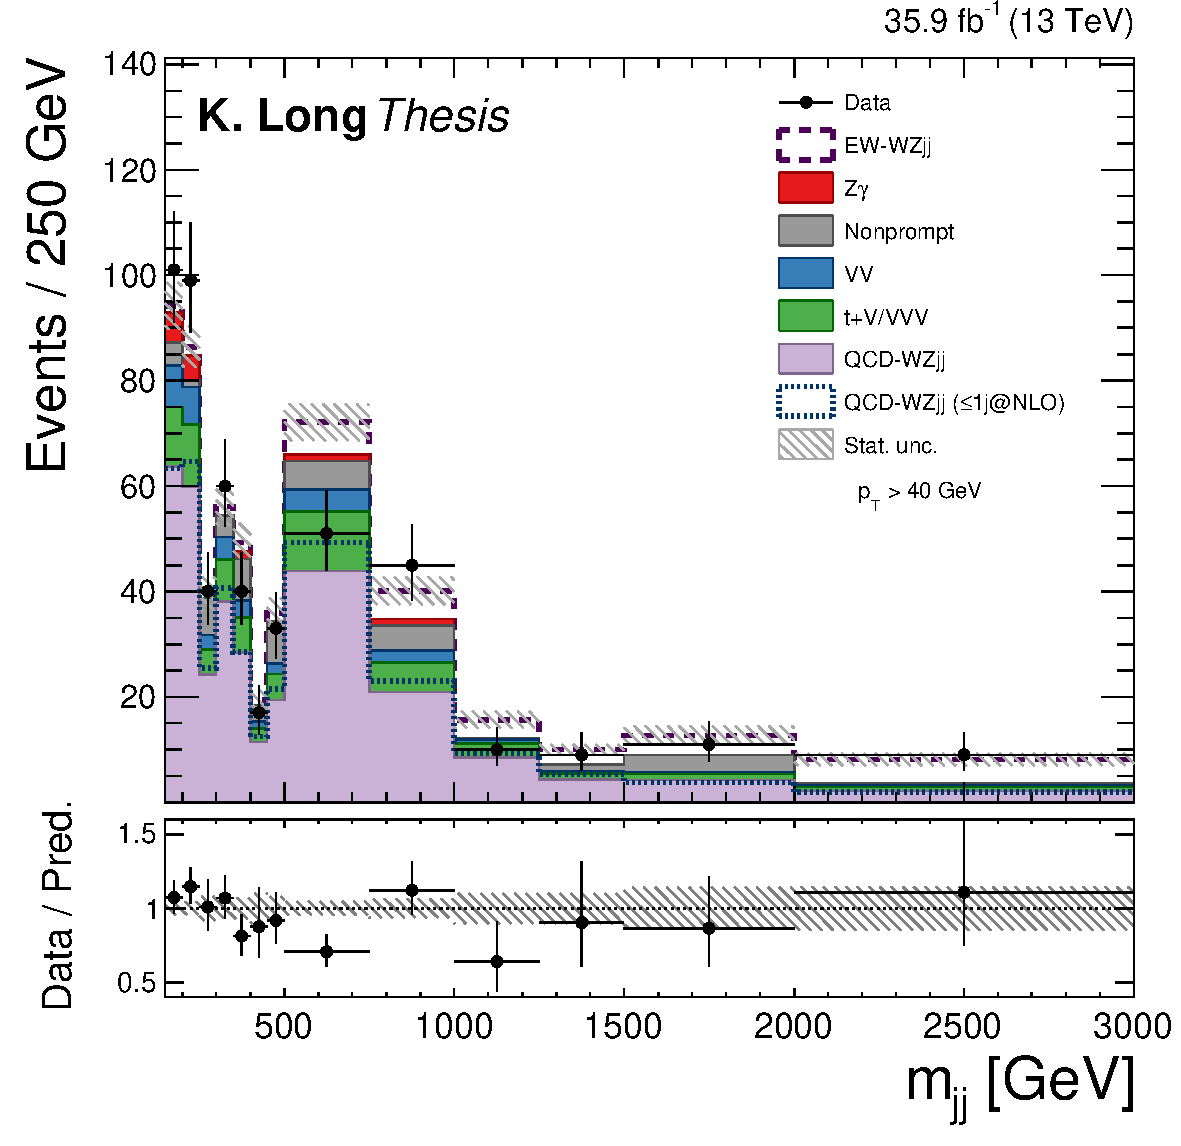
\includegraphics[width=0.49\textwidth]{figures/Conclusions/mjj_nMinus1_ATLASptj_Prefit.pdf}
   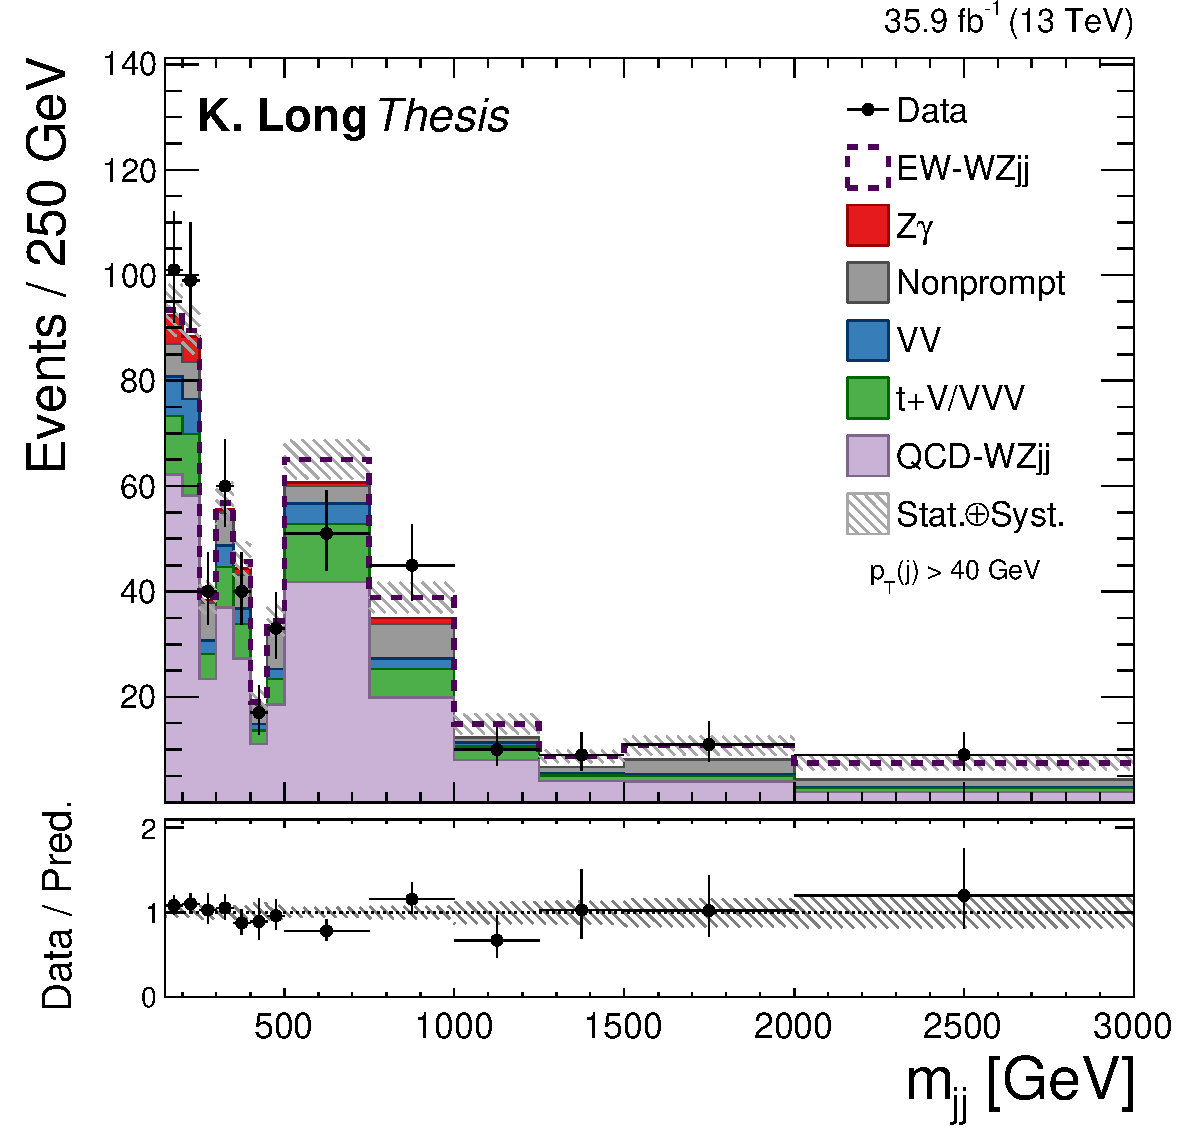
\includegraphics[width=0.49\textwidth]{figures/Conclusions/mjj_nMinus1_ATLASptj_Postfit.pdf}
  \caption[The $\mjj$ for events selected in a fiducial region designed to approximate the selection of the ATLAS Collaboration]{
    The $\mjj$ spectrum for events selected in a relaxed fiducial region, described in the text,
    designed to be comparable to the
    selection used by the ATLAS Collaboration in Ref.~\cite{Aaboud:2018ddq}. The distribution
    is shown using the expected normalizations input to
    the maximum likelihood fit (left) and the with the best fit normalizations
    by bin obtained from the fit (right). The data are well described by the 
    shape and normalization predicted by the MC simulations 
    of the \EWWZ (dashed purple) and \QCDWZ (filled light purple) processes
    discussed in Chapter~\ref{ch:simulation}
        }
 \label{fig:EWWZATLASselection}
\end{figure}

The measurement that has been presented in this thesis is designed to be sensitive
to the \EWWZ process with a minimal theoretical dependence. This is highlighted in
Fig.~\ref{fig:EWWZATLASselection}, which shows the $\mjj$ for events in a relaxed
selection intended to mimic the fiducial region defined by the ATLAS experiment.
The selection is defined following Table~\ref{tab:selections}, the no condition on the
pseduorapidity separation of the jets and with the jet transverse momentum relaxed to 40\GeV. A maximum likelihood fit
is performed to this distribution with the approach described in Chapter~\ref{ch:analysis}.
While the distribution is less sensitive to the \EWWZ process than the two-dimensional
likelihood, the central value of the \EWWZ signal strength is within 10\% of the value
presented, well within the uncertainty of the measurement. The normalization correction of the
\QCDWZ process that maximizes the likelihood is consistent with the presented result and with
unity. The distribution is well-described by the MC simulation and background estimation,
as illustrated in Fig.~\ref{fig:EWWZATLASselection}, which shows the distributions input 
to the maximum likelihood fit and the resulting best-fit distributions.
Studies to determine if a multivariate discriminant, following the approach
of the ATLAS Collaboration, results in a different categorization of the events
as \EWWZ and \QCDWZ will be a topic of future studies.

\begin{figure}[htbp]
  \centering
   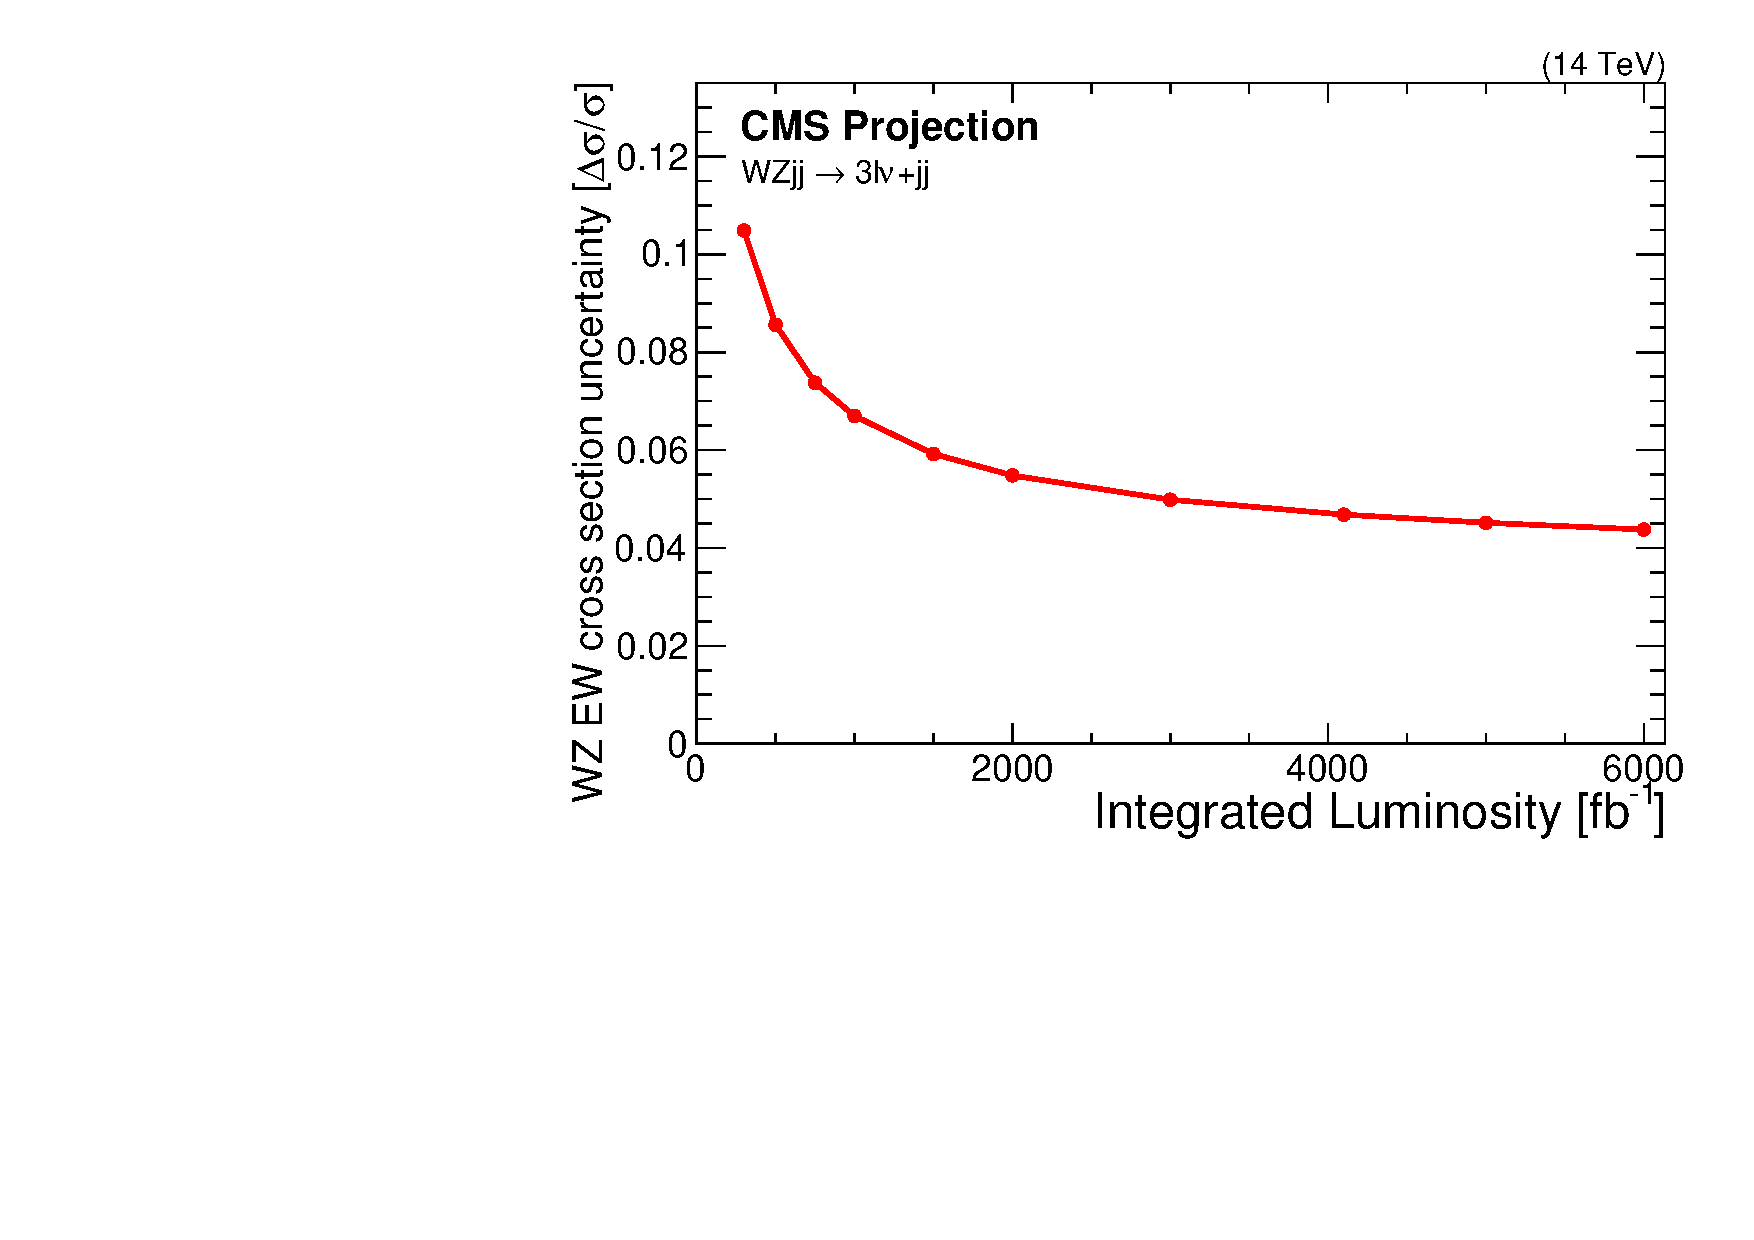
\includegraphics[width=0.6\textwidth]{figures/Conclusions/WZjjSignficanceHLLHC.pdf}
  \caption[Projected reduction in uncertainty for the \EWWZ cross section measurement at the HL-LHC]{
    Projected reduction in uncertainty for the \EWWZ cross section measurement 
    by the CMS detector at the HL-LHC. Reproduced from Ref.~\cite{CMS-PAS-FTR-18-038}.
        }
 \label{fig:WZHLLHC}
\end{figure}

The data set collected by the CMS experiment in 2016-2018 constitutes only a small fraction
of the data expected to be delivered by the LHC in its lifetime. Beginning at the end of 2020, the LHC
will resume collisions, likely at an increased energy of 14\TeV. A data set corresponding
to 300\fbinv is expected to be collected by 2023, at which point the LHC will be upgraded to
deliver 5--7 times the current instantaneous luminosities with the high-luminosity LHC (HL-LHC).
During more than ten years of data taking the HL-LHC targets 3000\fbinv of data.
This analysis has been projected to the HL-LHC data set by extrapolating the 
luminosity and correcting estimating the change in reconstruction efficiency 
due to the harsh pileup conditions at the HL-LHC in Ref.~\cite{CMS-PAS-FTR-18-038}.
As shown in Figure~\ref{fig:WZHLLHC}, measurements of the \EWWZ process will be possible with
percent-level precision. In addition, sensitivity to the longitudinally polarized 
components of the \EWWZ process, which is closely linked to electroweak symmetry
breaking and is sensitive to spin-dependent new physics, may be observable 
by combining high-precision predictions with innovative analysis techniques.

Sensitivity to physics beyond the SM will also improve with the increasing LHC data set. Constraints
on the production cross sections and operator couplings are expected to improve proportional to the square root
of the luminosity, provided the systematic uncertainties remain subdominant.
Resonant production of massive particles requires a parton-parton interaction
with sufficient energy to produce the resonance, therefore,
the observable mass range of charged Higgs bosons or other charged
resonances would be dramatically improved by an increase in scattering energy.
A high-energy upgrade of the LHC (HE-LHC) that achieves \pp collisions at $sqrt{s}=27\TeV$
by installing hypothetical 16\unit{T} magnets in the existing tunnel
has been proposed~\cite{Zimmermann:2647706}, following the completion of the 
HL-LHC project by 2040.
Ambitious proposals for a 100\TeV collider installed in a new 100\unit{km} tunnel at 
CERN or at a new location are also being considered~\cite{Mangano:2651294}.
It is almost universally accepted that new particles or interactions must exist between the electroweak scale 
set by $\sim m_{\PW} \sim m_{\PH}$ and the Planck Scale $\sim 10^{19}\GeV$,
however, unlike for the case of the Higgs boson and the LHC~\cite{RevModPhys.56.579}, 
a further restriction of this energy scale has not been convincingly established~\cite{Arkani-Hamed:2015vfh}.
With the current outlook for the field of particle physics, precision measurements, 
such as studies of the vector and Higgs boson couplings~\cite{Englert:2014uua,Anders:2018gfr}, 
remain exceedingly relevant.
Small deviations in observables sensitive to new interactions could point
to an energy scale of new particles, providing motivation and a target
energy regime for a new high-energy collider~\cite{Marciano_2002}. 


\SingleSpace{}
\setlength{\bibitemsep}{\onelineskip}
\printbibliography{}

\end{document}
